\documentclass{report}
\usepackage{amsmath}
\usepackage{amssymb}
\usepackage{amsthm}
\usepackage{czech}
\usepackage[bookmarks,bookmarksopen]{hyperref}
\usepackage{graphicx}%eps files
%\usepackage{a4wide}
\usepackage[textwidth=15cm, marginparwidth=2cm]{geometry}
\usepackage{url}% \path

\usepackage{algorithmic}
\usepackage[chapter]{algorithm}
\floatname{algorithm}{Algoritmus}
\renewcommand{\listalgorithmname}{Seznam algoritm�}

\newcommand{\pr}{{\cal P}}
\newcommand{\rozvoj}[3]{\binom{#1}{#2}\left(#3\right)^{#2}\left(1-#3\right)^{#1-#2}}
\newcommand{\invm}{\frac{1}{m}}
\newcommand{\intrange}[2]{\{{#1}\ ..\ {#2}\}}
\def\<#1>{\text{\it #1}} % viceznakova jmena promennych

\newcommand{\lparen}{(}
\newcommand{\rparen}{)}
{
\catcode`\(=13
\catcode`\)=13
\gdef({\left\lparen\begingroup}
\gdef){\endgroup\right\rparen}
\gdef\bigparens{%
	\catcode`\(=13%
	\catcode`\)=13%
}
}

\newcommand{\mnote}[1]{\marginpar{\scriptsize\raggedright #1}}
\newcommand{\exercise}[2]{\mnote{Cvi�en�: #1}} %TODO: co s odpov�d�?

\newtheorem{theorem}{V�ta}[section]
\newtheorem{lemma}{Lemma}[section]
\theoremstyle{definition}
\newtheorem{defn}{Definice}[section]

\pagestyle{myheadings}

%\includeonly{trees-ab}
\begin{document}

\title{Datov� struktury}
\author
{p�edn�� V�clav Koubek \and
z\TeX al Martin Vidner, Vladim�r Kotal
\footnote{\tt martin@artax.karlin.mff.cuni.cz, mvidner@atlas.cz}
\thanks{P�isp�li: Li��k, J��a, �abi�ka, Jind�ich, MJ, Pavel
	\ldots \emph{mus�m napsat po��dn� titulky}}
}
\maketitle
\tableofcontents
%\listofalgorithms

% ==========================================================================
% Sou��st skript na Datov� struktury. Viz main.tex
\markright{$ $Id$ $}

\chapter{�vod}

Chceme reprezentovat data, prov�d�t s nimi operace. C�lem t�to
p�edn�ky je popsat ideje, jak datov� struktury reprezentovat, popsat
algoritmy pracuj�c� s nimi a p�esv�d�it v�s, �e kdy� s nimi budete
pracovat, m�li byste si ov��it, jak jsou efektivn�.

Probl�m m��en� efektivity: v�t�inou nem�me �anci vyzkou�et v�echny
p��pady vstupn�ch dat. Mus�me bu� doufat, �e na�e vzorky jsou
dostate�n� reprezentativn�, nebo to vypo��tat. Tehdy ale zase nemus�me
dostat p�esn� v�sledky, pouze odhady.

% --------------------------------------------------------------------------
\section{P�edpoklady}

\begin{enumerate}
\item Datov� struktury jsou nez�visl� na �e�en�m probl�mu;
abstrahujeme. Nap��klad u slovn�kov�ch operac� {\it vyhledej, p�idej,
vyjmi,\/} n�s nezaj�m�, jestli slovn�k reprezentuje body v prostoru,
vrcholy grafu nebo z�znamy v datab�zi.
\item V programu, kter� �e�� n�jak� probl�m, se p��slu�n� datov�
struktury pou��vaj� {\em velmi �asto}.
\end{enumerate}

% --------------------------------------------------------------------------
\section{Jak� typy slo�itosti n�s zaj�maj�}

\subsection{Pam�ov� slo�itost reprezentovan� struktury}
Je d�le�it�, ale obvykle jednoduch� na spo��t�n� a nen� �ance ji
vylep�it --- jedin� pou��t �pln� jinou strukturu. Proto ji �asto
nebudeme ani zmi�ovat.

\subsection{�asov� slo�itost algoritm�\\ pracuj�c�ch na datov� struktu�e}

\subsubsection{�asov� slo�itost v nejhor��m p��pad�}
Jej� znalost n�m zaru��, �e nem��eme b�t nep��jemn� p�ekvapeni (dobou
b�hu algoritmu). Hod� se pro {\em interaktivn�} re�im --- u�ivatel
sed�c� u datab�ze pr�m�rn� dobrou odezvu neocen�, ale jedin� pomal�
p��pad si zapamatuje a bude si st�ovat. Za vylep�en� nejhor��ho
p��padu obvykle plat�me zhor�en�m pr�m�rn�ho p��padu.

\subsubsection{O�ek�van� �asov� slo�itost}
Je to vlastn� v�en� pr�m�r --- slo�itost ka�d�ho p��padu vstupn�ch
dat n�sob�me pravd�podobnost� jeho v�skytu a se�teme. Je zaj�mav� pro
d�vkov� re�im zpracov�n�. Nap��klad Quicksort pat�� mezi nejrychlej�� zn�m�
t��d�c� algoritmy, ale v nejhor��m p��pad� m� slo�itost kvadratickou.

Pozor na p�edpoklady o rozd�len� vstupn�ch dat. Je zn�m� fakt, �e pro ka�d� 
$k$ existuje ��slo $n_k$ takov� �e ka�d� n�hodn� graf s alespo� $n_k$ vrcholy
s velkou pravd�podobnost� obsahuje kliku velikosti $k$. To vede k 
n�sleduj�c�mu algoritmu, kter� ur�� zda graf je nejv��e $k-1$ barevn� s 
o�ek�van�m konstantn�m �asem.

Algoritmus: vstup graf $(V,E)$.
\begin{enumerate}
\item
Kdy� velikost $V$ je men�� ne� $n_k$, pak prohled�n�m v�ech mo�nost� 
ur�i barevnost grafu $(V,E)$ a vydej odpov��, jinak pokra�uj na n�sleduj�c� 
bod.
\item
Zvol n�hodn� $n_k$ vrchol� v mno�in� $V$ a zjisti zda indukovan� podgraf 
na t�to mno�in� obsahuje kliku velikosti $k$. Pokud ano, odpov�� je ne, 
jinak pokra�uj na n�sleduj�c� bod.
\item
Prohled�n�m v�ech mo�nost� ur�i barevnost grafu $(V,E)$ a vydej odpov��.
\end{enumerate}


Tento algoritmus se ale pro praktick� pou�it� moc nehod�, proto�e norm�ln� 
se nap��klad s n�hodn�mi grafy na 200 vrcholech nesetk�v�me.

\subsubsection{Amortizovan� slo�itost}
Pro ka�d� $n$ nalezneme nejhor�� �as vy�adovan� posloupnost� $n$ 
operac� a tento �as vyd�l�me $n$. Amortizovan� slo�itost je limitou 
t�chto hodnot pro $n$ jdouc� do nekone�na. To n�s zaj�m� proto, �e n�kter�
datov� struktury maj� takovou vnit�n� organizaci, �e na n� z�vis�
slo�itost, a ta organizovanost se b�hem posloupnosti operac�
m�n�. Nejhor�� p��pad vlastn� ukl�z� za n�sleduj�c� nebo
p�edchoz� rychl� p��pady.

Nap��klad u p�i��t�n� jedni�ky ke $k$-cifern�mu bin�rn�mu ��slu je
�asov� slo�itost po�et jedni�ek ve vstupu. Nejhor�� p��pad s line�rn�
slo�itost� nastane pro ��slo ze sam�ch jedni�ek (tedy $2^k-1$), ale
t�ch p��pad� je m�lo a amortizovan� slo�itost nakonec vyjde
konstantn�.

Nebo ur�it� algoritmy v p�eklada��ch v praxi b�� rychle, p�esto�e
jednotliv� operace maj� velkou slo�itost v nejhor��m p��pad�. 
To se tak� poda�ilo vysv�tlit pomoc� amortizovan� slo�itosti.

\subsubsection{Asymptotick� notace}

Skute�n� slo�itost z�vis� na implementaci algoritmu, na konkr�tn�m
po��ta�i, vlastn� se ned� p�esn� spo��tat v obecn�m p��pad�. Abychom 
mohli spo��tat aspo� n�co, za�aly se pou��vat odhady slo�itosti a� 
na multiplikativn� konstantu. Tyto odhady popisuj� r�st slo�itosti 
vzhledem ke zv�t�uj�c�m se vstup�m, ale neur�uj� konkr�tn� funkci 
(��sla). 

Nech� $f, g$ jsou funkce na p�irozen�ch ��slech. Zna��me:
\begin{eqnarray}
f = O(g),	&\text{kdy� }
	&\exists c>0 \ \forall n: f(n) \leq c g(n) \\
f = \omega(g)	&
	&\forall c>0 \ \exists \text{nekone�n� mnoho }n: f(n) > c g(n)\\
f = \Theta(g)	&
	&\exists c,d>0 \ \forall n: d g(n) \leq f(n) \leq c g(n)
\end{eqnarray}

Budeme p�ev�n� pou��vat $O$, proto�e chceme hlavn� horn� odhady, kde�to doln�
odhady b�v� obvykle t쾹� zjistit. Pro �plnost:
\[ f=o(g), \text{kdy� } \lim_{n \to \infty} \frac{f(n)}{g(n)} = 0 \]


% ==========================================================================
\chapter{Slovn�kov� probl�m}

Je d�no universum $U$, m�me reprezentovat jeho podmno�inu $S \subseteq
U$.

\newcommand{\MEMBER}{\text{MEMBER}}
\newcommand{\INSERT}{\text{INSERT}}
\newcommand{\DELETE}{\text{DELETE}}
Budeme pou��vat operace
\begin{itemize}
\item $\MEMBER(x), x \in U,$ 
	odpov�� je {\em ano,} kdy� $x \in S$, {\em ne,} kdy� $x \notin S$.
\item $\INSERT(x), x \in U,$ 
	vytvo�� reprezentaci mno�iny $S \cup \{x\}$
\item $\DELETE(x), x \in U,$ 
	vytvo�� reprezentaci mno�iny $S \setminus \{x\}$
\item ACCESS($x$). Ve skute�n�ch datab�z�ch MEMBER nesta��, proto�e se
krom� kl��e prvku zaj�m�me i o jeho ostatn� atributy. Tady se ale o n�
starat nebudeme --- obvykl� �e�en� je m�t u kl��e pouze ukazatel na
ostatn� data, co� usnad�uje p�em�s�ovan� jednotliv�ch prvk� datov� struktury.
\end{itemize}

P�edpokl�d� se znalost t�chto z�kladn�ch datov�ch struktur: pole,
spojov� seznam, obousm�n� seznam, z�sobn�k, fronta, strom.

% --------------------------------------------------------------------------
\section{Pole}

Do pole velikosti $|U|$ ulo��me charakteristickou funkci $S$.
\begin{itemize}
\item[+] Velmi jednoduch� a rychl� --- v�echny operace prob�haj� v
konstantn�m �ase $O(1)$
\item[--] Pam�ov� n�ro�nost $O(|U|)$, co� je k�men
�razu. Nap�. datab�ze v�ech lid� v �esku, k�dovan�ch rodn�m ��slem, by
snadno p�erostla mo�nosti 32-bitov�ho adresn�ho prostoru (10 miliard
R� $\times$ 4B ukazatel) \mnote{Naj�t lep�� p��klad?} Ale pro grafov�
algoritmy je tahle reprezentace velmi vhodn�.
\end{itemize}

% --------------------------------------------------------------------------
\section{Seznam}

Vytvo��me seznam prvk� v $S$, operace prov�d�me prohled�n�m
seznamu. �asov� i pam�ov� slo�itost operac� je $O(|S|)$ (a to i pro
INSERT --- mus�me zjistit, jestli tam ten prvek u� nen�).

% ==========================================================================
% Sou��st skript na Datov� struktury. Viz main.tex
\markright{$ $Id$ $}

\def\prazdnatabulka{
\begin{tabular}{|l|l|}
\hline
& kl��\\
\hline
0& \\
1& \\
2& \\
3& \\
4& \\
5& \\
6& \\
7& \\
8& \\
9& \\
\hline
\end{tabular}
}

\chapter{Ha�ov�n� I}

Je d�no universum $U$, reprezentovan� podmno�ina $S, S \subseteq U, |S|=n$.
Velikost tabulky, ve kter� budeme cht�t $S$ reprezentovat je $m$. 

M�me ha�ovac� funkci $h: U \to \{0..m-1\}$. Mno�ina $S$ je
reprezentov�na tabulkou $T[0..m-1]$ tak, �e prvek $s \in S$ je ulo�en na
m�st� $h(s)$.

Charakteristickou vlastnost� obecn� ha�ovac� funkce je velk� pl�tv�n� 
pam�t� pokud $n \ll |U|$, nap�. pro $n = \log\log |U|$.

S prvky, kter� nesou kladnou informaci ($x \in S$), moc
nenad�l�me. Ale z�porn� m��eme n�jak slou�it do jednoho nebo i
p�ekr�t s t�mi kladn�mi. To je z�kladn� idea ha�ov�n�.


Probl�my:
\begin{enumerate}
\item Jak rychle spo��t�me $h(s)$.
\item Co znamen� {\em ulo�en na m�st� $h(s)$} ? Co kdy� plat� $h(s)=h(t)$
a z�rove� $s \ne t$ ?
\end{enumerate}

�e�en�:
\begin{enumerate}
\item Omez�me se na rychle spo�itateln� ha�ovac�
funkce. P�edpokl�d�me, �e $h(s)$ spo�teme v �ase $O(1)$.
\item Tento p��pad se naz�v� {\em kolize} a jednotliv� druhy ha�ov�n�
se d�l� podle toho, jak �e�� kolize.
\end{enumerate}

% --------------------------------------------------------------------------
\section{Ha�ov�n� se separovan�mi �et�zci}

Tento zp�sob ha�ov�n� �e�� kolize tak, �e koliduj�c� prvky ukl�d� na
stejnou pozici do tabulky. Na t�to pozici jsou ulo�eny v podob� 
line�rn�ch seznam�. Takov�mu seznamu koliduj�c�ch prvk� se ��k�
\emph{�et�zec}.
Ha�ovac� tabulka je tedy pole line�rn�ch seznam�, ne nutn� uspo��dan�ch.
Odtud plyne n�zev t�to metody, proto�e �et�zce prvk� nejsou mezi sebou
prom�ch�ny - �et�zec, kter� je v tabulce ulo�en na pozici $y$ v sob� 
obsahuje pouze ty prvky, pro kter� plat� $h(x) = y$.

Z�kladn� operace na t�to tabulce jsou MEMBER (viz algoritmus
\ref{alg:hash1.separ.member}),
INSERT (viz alg. \ref{alg:hash1.separ.insert}) a DELETE (viz alg. 
\ref{alg:hash1.separ.delete}).

\begin{algorithm}[!htb]
\caption{MEMBER pro ha�ov�n� se separovan�mi �et�zci}
\label{alg:hash1.separ.member}
MEMBER(x):
\begin{enumerate}
\item Spo��t�me $h(x)$.
\item Prohled�me $h(x)$-t� seznam.
\item Kdy� tam $x$ je, vr�t�me {\em true}, jinak {\em false}.
\end{enumerate}
\end{algorithm}


\begin{algorithm}[!htb]
\caption{INSERT pro ha�ov�n� se separovan�mi �et�zci}
\label{alg:hash1.separ.insert}
INSERT(x):
\begin{enumerate}
\item Spo��t�me $h(x)$. {\it (Jako MEMBER)}
\item Prohled�me $h(x)$-t� seznam. {\it (Jako MEMBER)}
\item Kdy� $x$ nen� v $h(x)$-t�m seznamu, tak ho tam vlo��me.
\end{enumerate}
\end{algorithm}


\begin{algorithm}[!htb]
\caption{DELETE pro ha�ov�n� se separovan�mi �et�zci}
\label{alg:hash1.separ.delete}
DELETE(x):
\begin{enumerate}
\item Spo��t�me $h(x)$. {\it (Jako MEMBER)}
\item Prohled�me $h(x)$-t� seznam. {\it (Jako MEMBER)}
\item Kdy� $x$ je v $h(x)$-t�m seznamu, tak ho odstran�me.
\end{enumerate}
\end{algorithm}


O�ek�van� doba operace MEMBER, INSERT nebo DELETE 
je stejn� jako o�ek�van� d�lka seznamu.
Ale pozor na pr�zdn� seznam, u n�j nedos�hneme nulov�ho �asu operace. 
Uk�eme, �e o�ek�van� doba operace je konstantn�.

\begin{samepage}
P�edpoklady:
\begin{enumerate}
\item $h$ rozd�luje prvky $U$ do seznam� nez�visle a rovnom�rn�
(nap�. $h(x) = x \bmod m$).\\
Tedy pro $\forall {i,j}:{0 \leq i,j < m}$ se 
po�ty prvk� $S$ zobrazen�ch na $i$ a $j$ li�� nejv�� o 1.
\item Mno�ina $S$ m� rovnom�rn� rozd�len� --- v�b�r konkr�tn� mno�iny
$S$ m� stejnou pravd�podobnost. To je dost omezuj�c�, proto�e na
rozd�l od ha�ovac� funkce nejsme schopni $S$ ovlivnit.
\end{enumerate}
\end{samepage}

% ..........................................................................
\subsection{O�ek�van� d�lka seznamu}

Ozna�me $p(\ell) = \pr(\hbox{seznam je dlouh� }\ell)$.

Z p�edpoklad� m� $p(\ell)$ binomick� rozd�len�, neboli
\[
p(\ell) = \rozvoj{n}{\ell}{\invm}
\]

\begin{samepage}
tedy o�ek�van� d�lka seznamu je
\begin{multline}\bigparens
\label{binom-uprava}
E 
= \sum_{\ell=0}^n \ell \cdot p(\ell)\\
= \sum_{\ell=0}^n \ell \frac{n!}{\ell!(n-\ell)!} (\invm)^\ell (1-\invm)^{n-\ell}
= \sum_{\ell=0}^n n \frac{(n-1)!}{(\ell-1)! [(n-1) - (\ell-1)]!} (\invm)^\ell (1-\invm)^{n-\ell}\\
= \sum_{\ell=0}^n \frac nm \binom{n-1}{\ell-1}(\invm)^{\ell-1} (1-\invm)^{(n-1)-(\ell-1)}
= \frac nm \sum_{k=-1}^{n-1} \binom{n-1}{k} (\invm)^k
(1-\invm)^{(n-1)-k}\\
\text{README.1st: v�echny �pravy sm��uj� k tomuto sou�tu podle binomick� v�ty}\\
= \frac nm ( \invm + (1-\invm) )^{n-1}
= \frac nm
= \alpha,
\end{multline}

kde $\alpha = n/m$ je tzv.~\emph{faktor napln�n�}\footnote{anglicky
\emph{load factor}}, obvykle je d�le�it�, je-li v�t�� �i men�� ne� 1.
\end{samepage}

\def\xx{
s rozptylem
{\bigparens $$ n \cdot \invm (1-\invm) $$}
}

% ..........................................................................
\subsection{O�ek�van� �as posloupnosti operac�}

Kdy� m�me posloupnost $P$ operac� MEMBER, INSERT, DELETE spl�uj�c�
p�edpoklad rovnom�rn�ho rozd�len� a aplikovanou na pr�zdnou ha�ovac�
tabulku, pak o�ek�van� �as je \( O( |P| + \frac{|P|^2}{2m} ) \)

% ..........................................................................
\subsection{O�ek�van� po�et test�}

\mnote{co je to test? porovn�n� kl���, nahl�dnut� do tabulky?}
Slo�itost prohled�n� seznamu se m��e li�it podle toho, jestli tam hledan�
prvek je nebo nen�. \emph{�sp�n�m p��padem} nazveme takovou Operaci(x), 
kde $x \in S$, \emph{ne�sp�n� p��pad} je $x \notin S$. V �sp�n�m p��pad�
prohled�v�me pr�m�rn� jenom polovinu seznamu.


O�ek�van� �as pro ne�sp�n� p��pad 
\( \text{E�N} = O( {(1 - \invm)}^n + \frac nm ) \)

O�ek�van� �as pro �sp�n� p��pad 
\( \text{E��} = O(\frac n{2m}) \)

\subsubsection{Ne�sp�n� p��pad}

Projdeme cel� seznam, mus�me nahl�dnout i do pr�zdn�ho seznamu.

$$ 
\text{E�N}
= 1 \cdot p(0) + \sum_{\ell=1}^n \ell \cdot p(\ell)
=         p(0) + \sum_{\ell=0}^n \ell \cdot p(\ell)
= (1-\invm)^n + \frac nm
\approx e^{-\alpha} + \alpha
$$

\subsubsection{�sp�n� p��pad}

\mnote{Zde Koubkov� 1998. Koubek 2000 to m� trochu jinak}

Po�et test� pro vyhled�n� v�ech prvk� v seznamu d�lky $\ell$ je\\
$1+2+\cdots+\ell = \binom{\ell+1}{2}$.

\def\OcPocTst{\sum_\ell \binom{\ell+1}{2} p(\ell)}
O�ek�van� po�et test� je $ \OcPocTst $, 
o�ek�van� po�et test� pro vyhled�n� v�ech prvk� v tabulce je
$ m \cdot \OcPocTst $.

Je�t� budeme pot�ebovat n�sleduj�c� sumu, kterou spo��t�me podobn�
jako v \ref{binom-uprava}:
$$ \sum_{l=0}^n l^2 \rozvoj{n}{l}{\invm}
= \cdots =
\frac{n}{m} (1-\invm) + (\frac{n}{m})^2
$$

O�ek�van� po�et test� pro vyhled�n� jednoho prvku
\begin{multline}
\text{E��}
= \frac{m}{n} \OcPocTst 
= \frac{m}{n} \cdot \frac{1}{2} ( \sum_\ell \ell^2 p(\ell) + \sum_\ell \ell \cdot p(\ell) )\\
= \frac{m}{2n} 
	( \frac{n}{m} (1-\invm)
	+ \frac{n^2}{m^2} 
	+ \frac{n}{m}
	)\\
= \frac{1}{2} - \frac{1}{2m} + \frac{n}{2m} + \frac{1}{2}
= 1 + \frac{n-1}{2m}\\
\sim 1 + \frac{\alpha}{2}
\end{multline}

% ..........................................................................
\subsection{O�ek�van� d�lka nejdel��ho seznamu}

\begin{samepage}
Zn�me o�ek�van� hodnoty, ale ty n�m samy o sob� moc ne�eknou. Hodila
by se n�m standardn� odchylka, ta se ale slo�it� po��t�. M�sto toho
vypo�teme o�ek�van� nejhor�� p��pad:

Dok�eme, �e
za p�edpoklad� 1 a 2 a $|S| = n \leq m$ je o�ek�van� d�lka maxim�ln�ho
seznamu $\text{EMS} = O( \frac{\log n}{\log\log n} )$.
\end{samepage}

Z definice 
\[
\text{EMS} = \sum_j j \cdot \pr(\text{maxim�ln� d�lka seznamu}=j). 
\]
Pou�ijeme trik: nech� 
\[
q(j) = \pr(\text{existuje seznam, kter� m� d�lku alespo� }j). 
\]
Pak 
\[ \pr(\text{maxim�ln� d�lka seznamu}=j) = q(j) - q(j+1) \]
a
\[
\text{EMS} = \sum_j q(j) 
\] (teleskopick� suma) \mnote{vysv�tlit}

Spo�teme $q(j)$:
\[
q'(j) 
= \pr( \text{dan� seznam m� d�lku alespo� }j ) 
\leq \binom nj {(\frac 1m)}^j
\]
\[
q(j) \leq m \cdot q'(j)
\]
\[
\text{EMS}
\leq \sum \min(1, m \binom nj {(\frac 1m)}^j )
\leq \sum \min(1, m {(\frac nm)}^j \frac 1{j!} )
\leq \sum \min(1, \frac n{j!} )
\]

Nech�
\[
j_0 
=    \max\{k: k! \leq n \}
\leq \max\{k: (k/2)^{k/2} < n \}
= O( \frac{\log n}{\log\log n} ), 
\]
pak
\begin{multline}
\text{EMS}
\leq \sum_{j+0}^{j_0} 1 + \sum_{j=j_0}^\infty \frac n{j!}
=    j_0 + \sum_{j=j_0}^\infty \frac n{j_0!} \frac{j_0!}{j!}\\
\leq j_0 + \sum_{j=j_0}^\infty \frac{j_0!}{j!}
\leq j_0 + \sum_{j=j_0}^\infty (\frac 1{j_0})^{(j-j_0)} % geom �ada
\leq j_0 + \frac 1{1 - 1/j_0}\\
= O(j_0) = O ( \frac{\log n}{\log\log n} )
\qed
\end{multline}


% --------------------------------------------------------------------------
\section{Ha�ov�n� s uspo��dan�mi �et�zci}

Uspo��d�n� �et�zc� vylep�� ne�sp�n� p��pad, proto�e hled�n� v �et�zci
m��eme zastavit v okamziku, kdy naraz�me na prvek v�t�� ne� hledan� prvek
(za p�edpokladu, �e prvky v �et�zci jsou uspo��d�ny vzestupn�).

\subsection{O�ek�van� �as}

O�ek�van� �as v ne�sp�n�m p��pad� se od �asu v �sp�n�m p��pad� li��
jen o aditivn� konstantu.

%(Jenom citace v�ty z \cite{Vitter-Chen})

% --------------------------------------------------------------------------
\section{Ha�ov�n� s p�esuny}

Zat�m jsme p�edpokl�dali, �e �et�zce koliduj�c�ch prvk� jsou ulo�eny
n�kde v dynamicky alokovan� pam�ti. 
To nen� v�hodn�, proto�e vy�aduje pou�it� dal�� pam�ti i kdy� n�kter� 
�et�zce jsou pr�zdn�.
Proto nyn� budeme uk�dat �et�zce p��mo v tabulce.

�et�zec na $i$-t�m m�st� ulo��me do tabulky tak, �e 
prvn� prvek je na $i$-t�m m�st� a
pro ka�d� prvek �et�zce je v polo�ce {\tt vp�ed} adresa n�sleduj�c�ho prvku
�et�zce a v polo�ce {\tt vzad} je adresa p�edchoz�ho prvku. Za��tek,
resp. konec �et�zce m� pr�zdnou polo�ku {\tt vzad}, resp. {\tt vp�ed}.

\begin{samepage}
\begin{priklad}
Nap��klad pro $U=\mathbb{N}, m=10, h(x) = x \bmod 10$, ha�ujeme posloupnost
10, 50, 21, 60: 

\vspace{5mm}
\begin{tabular}{|l|l|l|l|}
\hline
& kl��& {\tt vp�ed}& {\tt vzad}\\
\hline
0& 10& 5& \\
1& 21& & \\
2& & & \\
3& 50& & 5\\
4& & & \\
5& 60& 3& 0\\
6& & & \\
7& & & \\
8& & & \\
9& & & \\
\hline
\end{tabular}
\end{priklad}
\end{samepage}
\vspace{5mm}

MEMBER(x) je jednoduch� - od $h(x)$-t�ho m�sta proch�z�me �et�zec prvk� a�
na konec a v p��pad� nalezen� prvku operaci ukon��me.

P�i INSERT mus�me zjistit, zda $h(x)$-t� �et�zec za��n� na $h(x)$-t�m
m�st�\footnote{To je jednoduch� - pokud prvek na $h(x)$-t�m m�st� m�
nulov� ukazatel {\tt vzad}, pak je za��tkem $h(x)$-t�ho �et�zce.}.
Pokud ano, prvek p�id�me do $h(x)$-t�ho �et�zce,
pokud ne, p�em�st�me prvek na $h(x)$-t�m m�st� na jin� voln� m�sto,
uprav�me {\tt vp�ed} a {\tt vzad} a prvek vlo��me na $h(x)$-t� m�sto.

% vynuceny zlom stranky, nechtel si dat rict pomoci samepage
\pagebreak

\begin{samepage}
\begin{priklad}
Tabulka z p�edchoz�ho p��kladu po INSERT(53) bude vypadat takto: 

\vspace{5mm}
\begin{tabular}{|l|l|l|l|}
\hline
& kl��& {\tt vp�ed}& {\tt vzad}\\
\hline
0& 10& 5& \\
1& 21& & \\
2& & & \\
3& 53& & \\
4& 50& & 5\\
5& 60& 4& 0\\
6& & & \\
7& & & \\
8& & & \\
9& & & \\
\hline
\end{tabular}
\end{priklad}
\end{samepage}
\vspace{5mm}

P�i DELETE mus�me testovat, zda odstra�ovan� prvek nen� na 1. m�st�
sv�ho �et�zce
a pokud ano a �et�zec m� v�ce prvk�, mus�me p�esunout jin� prvek z
tohoto �et�zce na m�sto odstra�ovan�ho prvku.

Jak zjist�me, �e jin� prvek $y$ pat�� tam, kde je ulo�en? 
\mnote{Tady m�m zmatek. Zav�st lep�� zna�en�.}
Spo��tat $h(y)$
m��e b�t relativn� pomal�. Pokud {\tt T[i].vzad} n�kam ukazuje, pak
v�me, �e $h(y) \ne h(x)$.


% --------------------------------------------------------------------------
\section{Ha�ov�n� se dv�ma ukazateli}

P�i ha�ov�n� s p�esuny ztr�c�me �as pr�v� t�mi p�esuny, obzvl�t�,
kdy� jsou z�znamy velk�. To motivuje n�sleduj�c� implementaci 
ha�ov�n� s �et�zci.

Pou�ijeme dva ukazatele, {\tt vp�ed} a {\tt za��tek}:
\begin{itemize}
  \item {\tt T[i].vp�ed} je index n�sleduj�c�ho prvku v �et�zci, 
  	kter� je zde ulo�en. (Nemus� to b�t �et�zec s $h(x)=i$.)
  \item {\tt T[i].za��tek} je index za��tku �et�zce, kter� obsahuje
  	prvky, jejich� $h(x)=i$.
\end{itemize}

\begin{priklad}
Nech� $h(x) = x \bmod 10$. Ukl�d�me prvky 50, 90, 31, 60:

\vspace{5mm}

\begin{tabular}{|l|l|l|l|}
\hline
& kl��& vp�ed& za��tek\\
\hline
0& 50& 3& 0\\
1& 31& & 1\\
2& 60& & \\
3& 90& 2& \\
4& & & \\
5& & & \\
6& & & \\
7& & & \\
8& & & \\
9& & & \\
\hline
\end{tabular}

\vspace{8mm}

% opet, samepage nefunguje
\pagebreak

\begin{samepage}
P�id�me 42, 72, 45:

\vspace{5mm}

\begin{tabular}{|l|l|l|l|}
\hline
& kl��& vp�ed& za��tek\\
\hline
0& 50& 3& 0\\
1& 31& & 1\\
2& 60& & 5\\
3& 90& 2& \\
4& 45& & \\
5& 42& 6& 4\\
6& 72& & \\
7& & & \\
8& & & \\
9& & & \\
\hline
\end{tabular}
\end{samepage}
\end{priklad}


% --------------------------------------------------------------------------
\section{Ha�ov�n� s line�rn�m p�id�v�n�m}

Jde to i bez ukazatel�.

Je d�no $m$ m�st, kter� tvo�� tabulku. Pokud je p��slu�n� pol��ko ji�
zapln�no, hled�me cyklicky prvn� voln� n�sleduj�c� m�sto a tam
zap��eme. Vhodn� pro m�lo zapln�nou tabulku ($<60\%$, pro $80\%$ 
vy�aduje u� hodn� �asu). T�m�� nemo�n� DELETE: bu� ozna�it m�sto jako smazan�, nebo
cel� p�eha�ovat. 

%\subsection{O�ek�van� po�et test�}
%(Jenom citace v�ty z Knutha, dk na cvi�en�)

\vspace{5mm}

\begin{tabular}{|l|l|}
\hline
& kl��\\
\hline
0& 120\\
1& 51\\
2& 72\\
3& \\
4& \\
5& \\
6& \\
7& \\
8& \\
9& \\
\hline
\end{tabular}

\vspace{8mm}

P�id�me 40, 98, 62, 108:

\vspace{5mm}

\begin{tabular}{|l|l|}
\hline
& kl��\\
\hline
0& 120\\
1& 51\\
2& 72\\
3& 40\\
4& 62\\
5& \\
6& \\
7& \\
8& 98\\
9& 108\\
\hline
\end{tabular}


% --------------------------------------------------------------------------
\section{Ha�ov�n� se dv�ma funkcemi (otev�en� h., h. s otev�enou adresac�)}

Pou�ijeme dv� ha�ovac� funkce, $h_1$ a $h_2$, je zde v�ak ��eln� p�edpokl�dat, 
�e $h_2(i)$ a $m$ jsou nesoud�ln� pro ka�d� $i\in U$. P�i INSERTu pak hled�me
nejmen�� $j$ takov�, �e $T[h_1(x) + j h_2(x)]$ je voln�.

\begin{priklad}
M�jme $h_1(x) = x \bmod 10$

\vspace{5mm}

\begin{tabular}{|l|l|}
\hline
& kl��\\
\hline
0& 10\\
1& 31\\
2& \\
3& \\
4& \\
5& \\
6& \\
7& \\
8& \\
9& \\
\hline
\end{tabular}

\vspace{5mm}

INSERT(100): $h_1(100)=0$ a p�edpokl�dejme, �e $h_2(100)=3$. Voln�
m�sto najdeme pro $i=1$.

INSERT(70): $h_1(70)=0$ a p�edpokl�dejme, �e $h_2(70)=1$. Voln�
m�sto najdeme pro $i=2$.

\vspace{5mm}

\begin{tabular}{|l|l|}
\hline
& kl��\\
\hline
0& 10\\
1& 31\\
2& 70\\
3& 100\\
4& \\
5& \\
6& \\
7& \\
8& \\
9& \\
\hline
\end{tabular}
\end{priklad}

\vspace{5mm}

Neuvedli jsme explicitn� vzorec pro $h_2$. Jej� sestaven� je toti�
slo�it�j��. V�imn�te si, �e nem��eme vz�t $h_2(100)=4$. V�echny
hodnoty $h_2$ toti� mus� b�t nesoud�ln� s velikost� tabulky.

\def\xx{
Nap�.: $h(i) = i \bmod 10$, \( h_1(i) = \begin{cases}
1 &\text{kdy�}\ i \equiv 1 \pmod 3 \\
3 &\text{kdy�}\ i \equiv 0 \pmod 3 \\
7 &\text{kdy�}\ i \equiv 2 \pmod 3
\end{cases}
\)
}

\subsection{Algoritmus INSERT}
% \mnote{Je�t� rozmyslet zna�en� a sjednotit z�pis algoritm�}

viz algoritmus \ref{alg:hash1.2fce.insert}.

\begin{algorithm}[!htb]
\caption{INSERT pro ha�ov�n� se dv�ma funkcemi}
\label{alg:hash1.2fce.insert}
INSERT(x)
\begin{enumerate}
\item 
 spo�ti $i=h_1(x)$
\item
 kdy� tam $x$ je, pak skon�i\\
 kdy� je m�sto pr�zdn�, vlo� tam $x$ a skon�i
\item 
 \begin{algorithmic}
 \IF {$i$-t� m�sto obsazeno prvkem $\ne x$}
 \STATE spo�ti $h_2(x)$
 \STATE $k = (h_1(x)+h_2(x)) \bmod m$
 \WHILE {$k$-t� m�sto je obsazen� prvkem $\ne x$ a $i\ne k$}
   \STATE \quad $k = (k+h_2(x)) \bmod m$
 \ENDWHILE
 \ENDIF
 \end{algorithmic}
\item
 kdy� je $k$-t� m�sto obsazen� prvkem $x$, pak ned�lej nic,\\ 
 kdy� $i=k$, pak ohla� p�epln�no, jinak vlo� $x$ na
 $k$-t� m�sto
\end{enumerate}
\end{algorithm}


Test $k\ne i$ v kroku 3 br�n� zacyklen� algoritmu. Tento probl�m m� 
alternativn� �e�en�, nedovol�me vlo�en� posledn�ho prvku (m�sto testu v  
cyklu si pamatujeme �daje nav�c). Analogick� probl�my nast�vaj� 
u ha�ov�n� s line�rn�m p�id�v�n�m. 

Tato metoda pracuje dob�e a� do 90\% zapln�n�.

\subsection{O�ek�van� po�et test�}

P�edpokl�d�me, �e posloupnost $h_1(x), h_1(x)+h_2(x), h_1(x)+2h_2(x), \dots$
je n�hodn�, tedy �e pro ka�d� $x$ maj� v�echny permutace ��dk� tabulky stejnou
pravd�podobnost, �e se stanou touto posloupnost�.

\subsubsection{p�i ne�sp�n�m vyhled�v�n�}

Ozna��me jej $C(n,m)$, kde $n$ je velikost reprezentovan� mno�iny a
$m$ je velikost ha�ovac� tabulky.

Bu� $q_j(n,m)$ pravd�podobnost, �e v tabulce velikosti $m$ s ulo�enou
mno�inou velikosti $n$ jsou p�i INSERT(x) obsazen� m�sta
$h_1(x)+ih_2(x)$ pro $i=0..j-1$ (tedy �et�zec m� alespo� $j$ prvk�).

\begin{multline}
C(n,m)	= \sum_{j=0}^n (j+1)(q_j(n,m) - q_{j+1}(n,m) \\
	=(\sum_{j=0}^n q_j(n,m) ) - (n+1) q_{n+1}(n,m)
	= \sum_{j=0}^n q_j(n,m)
\end{multline}
Proto�e
\begin{equation}
q_j(n,m) = \frac nm \frac{n-1}{m-1} \cdots \frac{n-j+1}{m-j+1}
	=  \frac nm q_{j-1}(n-1, m-1)
\end{equation}

dostaneme po dosazen�:
\begin{multline}
\ldots	= 1 + \sum_{j=1}^\infty \frac nm q_{j-1}(n-1, m-1)
	= 1 + \frac nm \sum_{j=1}^\infty q_{j-1}(n-1, m-1) \\
	= 1 + \frac nm C(n-1, m-1)
\end{multline}

�e�en�m tohoto rekurentn�ho vzorce je

\begin{equation}
C(n,m) = \frac{m+1}{m-n+1}, 
\end{equation}
co� dok�eme indukc�:
\begin{multline}
C(n,m)	= 1 + \frac nm C(n-1, m-1) \\
	= 1 + \frac nm \frac{m}{m-n+1} = \frac{m-n+1+n}{m-n+1} 
	= \frac{m+1}{m-n+1}
\approx   \frac 1{1-\alpha}
\end{multline}

\subsubsection{p�i �sp�n�m vyhled�v�n�}

Sou�et o�ek�van�ch test� v�ech INSERT� p�es vytv��en� reprezentovan�
mno�iny d�len� velikost� mno�iny.
\begin{multline}
= \frac 1n	\sum_{i=0}^{n-1} C(i, m)
= \frac 1n	\sum_{i=0}^{n-1} \frac{m+1}{m-i+1}
= \frac {m+1}n	\sum_{i=0}^{n-1} \frac    1{m-i+1} \\
= \frac {m+1}n
	((\sum_{i=1}^{m+1} \frac 1i) - (\sum_{i=1}^{m-n+1} \frac 1i))
\approx \frac {m+1}n \ln \frac{m+1}{m-n+1}
\approx \frac 1\alpha \ln \frac 1{1-\alpha}
\end{multline}

N�sleduj�c� tabulka d�v� o�ek�vanou dobu vyhled�v�n� pro r�zn� 
zapln�n� ha�ovac� tabulky.

\vspace{5mm}

\centerline{\begin{tabular}{c|cccccc}
$\alpha$ 
 & 0.5 & 0.7 & 0.9 & 0.95 & 0.99 & 0.999 \\
\hline
$\frac 1{1-\alpha}$ 
 & 2   & 3.3 & 10  & 20   & 100  & 1000 \\
$\frac 1\alpha \ln \frac 1{1-\alpha}$
 & 1.38& 1.7 & 2.55& 3.15 & 4.65 & 6.9
\end{tabular}}

% --------------------------------------------------------------------------
\section{Sr�staj�c� ha�ov�n� (standardn�: LISCH a EISCH)}

\mnote{XXX doplnit odhady pro �sp�n�/ne�sp�n� p��pad pro EISCH, LISCH, ..
z 2003/2004.}

Dal�� metodou jak �e�it kolize je neseparovat �et�zce. To znamen�, �e v
jednom �et�zci se nyn� mohou nach�zet prvky, kter� maj� r�zn� hodnoty
ha�ovac� funkce. Proto se t�to metod� ��k� \emph{sr�staj�c� ha�ov�n�}.
�et�zce se nep�esouvaj�, v tabulce tedy nemus� b�t obsa�ena informace 
kde za��n� dan� �et�zec.

Tabulka m� dv� polo�ky: kl�� a adresu n�sleduj�c�ho prvku ({\tt vp�ed}). 
Prvek $s \in S$ je reprezentov�n v �et�zci, kter� pokra�uje v m�st� $h(s)$.

\begin{priklad}
\label{priklad:srust.hash}
Op�t pou�ijeme ha�ovac� funkci $h(x) = x \mod 10$.
V n�sleduj�c� tabulce jsou srostl� �et�zce pro hodnoty 0 a 3 funkce $h$:

\vspace{5mm}

\begin{tabular}{|l|l|l|}
\hline
& kl��& {\tt vp�ed}\\
\hline
0& 10& 3\\
1& 21& \\
2& & \\
3& 40& 4\\
4& 33& 7\\
5& & \\
6& & \\
7& 70& \\
8& & \\
9& & \\
\hline
\end{tabular}
\end{priklad}

\vspace{5mm}

\subsection{Algoritmus INSERT}

viz algoritmus \ref{alg:hash1.srust.insert}

\begin{algorithm}[!htb]
\caption{INSERT pro sr�staj�c� ha�ov�n�}
\label{alg:hash1.srust.insert}
INSERT(x)
\begin{enumerate}
\item
 spo�ti $i=h(x)$
\item
 prohledej �et�zec za��naj�c� na m�st� $i$ a pokud nenajde� $x$,
 p�idej ho do tabulky a p�ipoj ho do toho �et�zce.
\end{enumerate}
\end{algorithm}

Kam do toho �et�zce m�me p�ipojit nov� prvek? (To je jin� ot�zka, ne�
kter� voln� m�sto zvolit.) Metoda LISCH (\emph{late insert standard 
coalesced hashing}) ho p�ipoj� na posledn� m�sto �et�zce, 
metoda EISCH (\emph{early insert standard coalesced hashing}) 
ho p�ipoj� hned za $h(x)$-t� m�sto.

\begin{priklad}
Po proveden� operac�
LISCH INSERT(103), EISCH INSERT(94) bude tabulka z p��kladu
\ref{priklad:srust.hash} vypadat takto:

\vspace{5mm}

\begin{tabular}{|l|l|l|}
\hline
& kl��& {\tt vp�ed}\\
\hline
0& 10& 3\\
1& 21& \\
2& & \\
3& 40& 4\\
4& 33& 6\\
5& & \\
6& 94& 7\\
7& 70& 9\\
8& & \\
9& 103& \\
\hline
\end{tabular}
\end{priklad}

\vspace{5mm}

\begin{pozn}
P�i �sp�n�m vyhled�n� je EISCH asi o 15\% rychlej�� ne� LISCH. (P�i
ne�sp�n�m jsou samoz�ejm� shodn�, proto�e v obou p��padech je nutn� 
proj�t cel� �et�zec.)
\end{pozn}

% XXX co s timto ?
\def\xx{
\subsection{Algoritmus MEMBER}
\subsection{Algoritmus INSERT LISCH}
\subsection{Algoritmus INSERT EISCH}
\subsection{O�ek�van� po�et test�}
(Jenom citace v�ty z~\cite{Vitter-Chen})
}

% --------------------------------------------------------------------------
\section{Sr�staj�c� ha�ov�n� s pomocnou pam�t� (obecn�: LICH, EICH, VICH)}

Standardn� sr�staj�c� ha�ov�n� m� tu nev�hodu, �e se p�i v�t��m
zapln�n� tabulky mohou vytvo�it dlouh� �et�zce. Tabulku tedy prodlou��me o
% tady bylo {\uv sklep} ale nejak to nefunguje XXX
pomocnou pam�t (tzv. \emph{sklep}), do kter� se nedostane ha�ovac� funkce, a
koliduj�c� prvky p�id�v�me odspodu. �et�zce tedy srostou a� po
zapln�n� sklepa.

Op�t existuj� varianty p�ipojen� nov�ho prvku do �et�zce: LICH a EICH
jsou analogick� k LISCH a EISCH. VICH (\emph{variable insert coalesced
hashing}) p�ipojuje na konec �et�zce, jestli�e �et�zec kon�� ve sklep�,
jinak na m�sto, kde �et�zec opustil sklep.

% opet, samepage nefunguje
\pagebreak

\begin{samepage}
\begin{priklad}
Provedeme operaci INSERT pro n�sleduj�c� posloupnost prvk�:
10, 41, 60, 70, 71, 90, 69, 40, 79. Tabulka pak bude vypadat takto:

% XXX \newcommand{\x}[1]{(#1)}
\vspace{5mm}

\begin{tabular}{|l||l|l||l|l||l|l|}
\hline
 & \multicolumn{2}{|c||}{LICH}& 
   \multicolumn{2}{|c||}{EICH}&
   \multicolumn{2}{|c|}{VICH}\\
\hline
 & kl��& {\tt vp�ed} & kl��& {\tt vp�ed} & kl��& {\tt vp�ed}\\
\hline
0&	10& 12&		10& (12)(11)(9)7& 10& 12\\
1&	41& 10&		41& 10&		41& 10\\
2&	& &		& &		& \\
3&	& &		& &		& \\
4&	& &		& &		& \\
5&	& &		& &		& \\
6&	79& &		79& 8&		79& 8\\
7&	40& 6&		40& 9&		40& 9\\
8&	69& 7&		69& 11&		69& \\
9&	90& 8&		90& (11)(8)6&	90& (8)6\\
\hline
10&	71& &		71& &		71& \\
11&	70& 9&		70& 12&		70& (9)7\\
12&	60& 11&		60& &		60& 11\\
\hline
\end{tabular}

\vspace{5mm}

Sklep je od "hlavn� ��sti" tabulky odli�en �arou.
\end{priklad}
\end{samepage}

\def\xx{%commented out
\begin{tabular}{|l|l|l|}
\hline
& kl��& {\tt vp�ed}\\
\hline
0& 10& 10\\
1& 41& 12\\
2& 90& 3\\
3& 62& \\
4& & \\
5& & \\
6& & \\
7& & \\
8& & \\
9& & \\
\hline
10& 60& 11\\
11& 70& 2\\
12& 71& \\
\hline
\end{tabular}
}%commented out


\subsection{Operace DELETE}

viz algoritmus \ref{alg:hash1.srust.pomoc.delete}

\begin{algorithm}[!htb]
\caption{DELETE pro sr�staj�c� ha�ov�n� s pomocnou pam�t�}
\label{alg:hash1.srust.pomoc.delete}
\begin{enumerate}
\item spo��t�me $h(x)$ a prohled�me �et�zec za��naj�c� na adrese $h(x)$. \\
kdy� neobsahuje $x$ $\rightarrow$ konec.
\item kdy� $x$ je na adrese $h(x)$ a v �et�zci n�sleduje prvek v pomocn� ��sti
tabulky (sklep�) - odstran�me $x$. Prvek, kter� n�sleduje za $x$ p�esuneme 
na m�sto $h(x)$ a uvoln�me jeho m�sto - konec.
\item $x$ je ve sklep� - zj�st�me, zda se nach�z� v �et�zci mimo sklep prvek
s ha�ovac� hodnotou $h(x)$ - pokud neexistuje, p�esuneme posledn� prvek v
�et�zci, kter� je ve sklep� na m�sto $x$ a m�sto posledn�ho prvku uvoln�me.
\par
Kdy� takov� prvek existuje, vezmeme prvn� prvek s touto vlastnost�.
Ozna�me ho $y$, pak $y$ p�eneseme na m�sto $x$ a budeme cht�t uvolnit m�sto
prvku $y$. (obrazn� �e�eno $x$ a $y$ v �et�zci prohod�me)
\item $x$ je v ��sti, kam m��e ha�ovac� funkce a �etezec v t�to ��sti
pokra�uje. pak $x$ odstran�me a prvky za $x$ zaha�ujeme do tabulky v po�ad�
jak se do n� ukl�daly a pokud vznik� kolize, um�st�me je zp�tky na m�sto,
kde byly.
\end{enumerate}
\end{algorithm}

% chci aby se priklad vlezl na jednu stranu
\pagebreak

\begin{priklad}
Pou�ijeme ha�ovac� funkci $h(x) = x \mod 10$

Provedeme operaci DELETE na prvky 41, 42.
\mnote{? 42 v puv. tabulce nebylo XXX sehnat puvodni priklad}

\begin{itemize}
\item metoda LICH: \\
odstran�me prvky 62,78,82,52 z �et�zce a provedeme postupn� 
INSERT: 62,78,82,52

\item metoda VICH: \\
odstran�me 62,78,82,52 a provedeme INSERT: 82,62,78,52.
pokud bychom provedli INSERT 82,62,52,78, pak bychom nepoznali, v jak�m to
bylo v tabulce po�ad�.
\end{itemize}

\vspace{5mm}

\begin{tabular}{|l||l|l|}
\hline
 & kl��& {\tt vp�ed} \\
\hline
0&	& \\
1&	11& 10\\
2&	32& 9\\
3&	43& \\
4&	& \\
5&	42& 9\\
6&	82& \\
7&	78& 6\\
8&	62& 7\\
9&	52& 8\\
\hline
10&	21& 11\\
11&	41& 12\\
12&	61& \\
\hline
\end{tabular}
\end{priklad}

\vspace{5mm}


\subsection{Srovn�vac� graf}

XXX
\mnote{Nascanovat obr�zek z Vittera a Chena~\cite{Vitter-Chen}}


% --------------------------------------------------------------------------
\section{Srovn�n� metod}

Zde uv�d�me porovn�n� podle po�tu test�, proto�e to se d�
{\em vypo��tat}. Doba b�hu se mus� {\em m��it}.

\subsection{Po�ad� podle ne�sp�n�ho p��padu}

\begin{samepage}
V ne�sp�n�m p��pad�:
\begin{enumerate}
\item h. s uspo��dan�mi �et�zci (nejlep��)
\item h. s p�esuny
\item VICH=LICH a h. se 2 ukazateli (VICH je lep�� a� do $\alpha=3/4$)
\item EICH
\item LISCH=EISCH (a� sem je v�e $O(1)$)
\item h. se 2 funkcemi
\item h. s line�rn�m p�id�v�n�m (nejhor��)
\end{enumerate}
\end{samepage}


\subsection{Po�et test� pro zapln�nou tabulku}

Po�et test� pro �pln� zapln�nou tabulku ($m=n$ nebo $m=n-1$)

\vspace{5mm}

\mnote{co znamenaj� ��sla v prav�m sloupci ?}
\begin{tabular}{|l|l|}
\hline
typ	& XXX \\
\hline
h. s p�esuny&		1.5\\
h. se 2 ukazateli&	1.6\\
VICH=LICH&		1.8\\
EICH&			1.92\\
LISCH=EISCH&		2.1\\
\hline
h. se 2 funkcemi&	$n$\\
h. s line�rn�m p�id�v�n�m&$n$\\
\hline
\end{tabular}

%\vspace{5mm}
%\bigskip

\subsection{Po�et test� vyj�d�en� vzorcem}

\begin{tabular}{|l|l|l|}
\hline
typ &�sp�n� vyhled�n� &ne�sp�n� hled�n�\\
\hline
s �et�zci &$ 1+\frac\alpha2 $ &$e^{-\alpha} + \alpha$\\
s uspo��dan�mi �et�zci &$ 1+\frac\alpha2 $ &
	$e^{-\alpha} + 1 + \frac\alpha2 - \frac1\alpha (1-e^\alpha)$\\
s p�emis�ov�n�m &$ 1+\frac\alpha2 $ &$e^{-\alpha} + \alpha$\\
se 2 ukazateli &$ 1 + \frac\alpha2 + \frac{\alpha^2}2 $ &
	$1 + \frac{\alpha^2}2 + \alpha + e^{-\alpha}(2+\alpha) - 2$\\
s line�rn�m p�id�v�n�m &$\frac12 (1 + \frac1{1-\alpha})$ &
	$\frac12 (1 + {(\frac1{1-\alpha})}^2 )$\\
dvojit� ha�ov�n� &$\frac 1\alpha \ln \frac 1{1-\alpha}$ &$\frac 1{1-\alpha}$\\
LISCH &\(\begin{aligned}
	 1 + \frac 1{8\alpha} (e^{2\alpha}-1-2\alpha)\\ + \frac14 \alpha
	\end{aligned}
	\)&
	$1+ \frac14 (e^{2\alpha}-1-2\alpha)$\\
EISCH &$\frac 1\alpha (e^\alpha - 1)$&
	$1+ \frac14 (e^{2\alpha}-1-2\alpha)$\\
\hline
\end{tabular}

\vspace{10mm}

% mimo tabulku, jinak to je hnus
LICH �sp�n�: 
 \(
 \begin{cases}
  1+ \frac \alpha{2\beta}
	&\text{kdy� } \alpha \leq \lambda\beta\\
  1
  +\frac\beta{8\alpha}(e^{2(\alpha/\beta-\lambda)}-1-2(\alpha/\beta-\lambda))\\
  \qquad \times (3 - \frac2\beta + 2\lambda)\\
  \quad + \frac14 (\frac\alpha\beta + \lambda)
  + \frac\lambda4 (1 - \frac{\lambda\beta}\alpha)
	&\text{kdy� } \alpha \geq \lambda\beta
 \end{cases}
 \)

LICH ne�sp�n�: 
 \(
 \begin{cases}
	e^{-\alpha/\beta} + \frac\alpha\beta 
		&\text{kdy� } \alpha \leq \lambda\beta\\
	\frac1\beta
	+ \frac14 (e^{2(\alpha/\beta-\lambda)}-1)(3 - \frac2\beta + 2\lambda)\\
	\quad - \frac12 (\alpha/\beta - \lambda)
		&\text{kdy� } \alpha \geq \lambda\beta 
 \end{cases}
 \),

kde $\beta = \frac m{m'}$ je pod�l adresov� ��sti tabulky na jej�
celkov� velikosti
a $\lambda$ je jedin� nez�porn� �e�en� rovnice 
$e^{-\lambda} + \lambda = \frac1\beta$.


% --------------------------------------------------------------------------
\section{P�eha�ov�v�n�}

V p�edchoz�ch metod�ch jsme narazili na p��pady, �e p�i velk�m
zapln�n� tabulky je nutn� ji p�eha�ovat. Zde si uk�eme metodu, jak se to
d�l�.

M�me ha�ovac� funkce: $h_0$ ha�uje do tabulky velikosti $m = 2^0 m$,
$h_1$ do $2m = 2^1 m$, $h_2$ do $4m = 2^2 m$ \ldots, $h_i$ do $2^i
m$.

% opet, samepage nezafungovalo
%\pagebreak
\vspace{10mm}

\begin{samepage}
\noindent
Mno�inu $S$ reprezentujeme takto:

Ulo�ena je velikost $S$ a ��slo $i$ takov�, �e
\begin{equation}
\label{prehas}
2^{i-2} m < |S| < 2^i m
\end{equation}
a S je zaha�ov�na funkc� $h_i$.
\end{samepage}

\subsection{MEMBER}

MEMBER funguje norm�ln�, p�i INSERT a DELETE kontrolujeme poru�en�
podm�nky \eqref{prehas} a p��padn� p�eha�ujeme pro $i \pm 1$:

\subsection{INSERT}

Provedeme operaci INSERT a kdy� m�me p�idat prvek, testujeme,
zda $|S|+1 < 2^i m$. Pokud nerovnost plat�, dokon��me INSERT. Pokud
neplat�, zv�t��me $i$ o 1 a spo��t�me ulo�en� $S \cup \{x\}$ vzhledem
k nov� ha�ovac� funkci $h_i$.

\subsection{DELETE}

Provedeme operaci DELETE a kdy� m�me odstranit prvek, testujeme,
zda $i>0$ a $|S|-1 = 2^{i-2} m$. Pokud rovnost neplat�, dokon��me DELETE. Pokud
plat�, zmen��me $i$ o 1 a spo��t�me ulo�en� $S - \{x\}$ vzhledem
k nov� ha�ovac� funkci $h_i$.

\subsection{Slo�itost}

Tato metoda m� malou amortizovanou slo�itost. Kdy� se spo��t� ha�ovac� 
tabulka pro novou ha�ovac� funkci $h_i$, pak obsahuje $2^{i-1}m$ prvk� a 
proto je t�eba alespo� $2^{i-2}m$ �sp�n�ch operac� DELETE nebo $2^{i-1}m$ 
�sp�n�ch operac� INSERT, abychom p�epo��t�vali tabulku pro jinou ha�ovac� 
funkci. Tedy amortizovan� slo�itost p�epo��t�v�n� tabulky je $O(1)$ (tato 
metoda nen� vhodn� pro pr�ci v interaktivn�m re�imu).


% ==========================================================================
% Sou��st skript na Datov� struktury. Viz main.tex
\markright{$ $Id$ $}

\chapter{Ha�ov�n� II}

% --------------------------------------------------------------------------
\section{Univerz�ln� ha�ov�n�}

Idea univerz�ln�ho ha�ovan� m� odstranit po�adavek na rovnom�rn� 
rozlo�en� vstupn�ch dat. Tento po�adavek chceme nahradit t�m, �e 
budeme m�t soubor $H$ ha�ovac�ch funkc� do tabulky velikosti $m$ takov�,
�e pro ka�dou podmno�inu $S$ univerza $U$ je pravd�podobnost, �e funkce z 
$H$ se chov� dob�e, hodn� velk� (tj. je jen m�lo koliz�). V tomto p��pad�, 
kdy� vybereme $h$ z $H$ n�hodn� s rovnom�rn�m rozlo�en�m, pak pro ka�dou 
podmno�inu $S\subseteq U$ takovou, �e $|S|\leq m$, bude o�ek�van� �as 
(po��tan� p�es v�echny funkce z $H$) konstantn�. Rozd�l proti tradi�n�mu 
ha�ovan� je, �e p�edpoklad rovnom�rn�ho v�b�ru ha�ovac� funkce z mno�iny 
$H$ m��eme zajistit (nebo se k spln�n� tohoto po�adavku p�ibl��it), ale 
v�b�r vstupn�ch dat ovlivnit nem��eme. Nyn� tuto ideu zformalizujeme. 
\mnote{zaj�m� n�s jednak $c$, jednak velikost syst�mu (tj. po�et funkc� v
syst�mu)}

\begin{defn}
\label{c-us}
T��da ha�ovac�ch funkc� 
\( H \subseteq \{h | h: \intrange{0}{N-1} \rightarrow \intrange{0}{m-1}\} \)
je \emph{c-univerz�ln�} syst�m, kde $c\in\mathbb{R}^+$, jestli�e 
\begin{equation*}
\forall x\neq y\in \intrange{0}{N-1} :
\left |\{h\in H : h(x)=h(y)\}\right| \leq c\frac{|H|}{m}, 
\end{equation*}
\end{defn}

%Doln� mez pro $c$, dk na cvi�en�.
% r�di bychom \( c \) co nejmen��, ale d� se dok�zat,
% �e neexistuj� \( c \)-univerz�ln� t��dy pro
% \( c<1-\frac{m}{N} \).

% ..........................................................................

\noindent
Nejprve uk�eme, �e $c$-univerz�ln� syst�my existuj�:

\begin{theorem}
P�edpokl�dejme, �e $U = \intrange{0}{N-1}$, kde $N$ je prvo��slo.
Definujme 
\[ H=\{h_{ab}:h_{ab}(x)=((ax+b)\bmod N)\bmod m;
\ a,b\in \intrange{0}{N-1}\} \]

Potom $H$ je \( c \)-univerz�ln� a 
\( c=\left( \left\lceil \frac{N}{m}\right\rceil /\frac{N}{m}\right) ^{2} \).
\end{theorem}

\begin{proof}
\( |H|=N^{2} \), co� je po�et dvojic $(a,b)$.

Nech� $(x,y)$ jsou libovoln�, ale pevn�. 
% oprava x != y by V. Havranek
Z�rove� plat� $x \neq y$.
Kolize nastane v p��padech, kdy�:

\[
h_{ab}(x)=h_{ab}(y),\]
neboli
\begin{eqnarray*}
ax+b & = & q+rm\pmod N\\
ay+b & = & q+sm\pmod N
\end{eqnarray*}

kde $(a,b)$ jsou nezn�m� a parametry $(q,r,s)$ nab�vaj� v�ech
hodnot takov�ch, �e
\[
q\in \intrange{0}{m-1}
\land r,s\in \intrange{0}{\left\lceil N/m\right\rceil -1}.
\]


$N$ je prvo��slo, tedy $\mathbb{Z}_N$ je t�leso a pro ka�dou trojici parametr�
$(q,r,s)$ m� soustava pr�v� jedno �e�en� $(a,b)$. 
Po�et koliduj�c�ch funkc� je p�esn� tolik, jako po�et trojic
$(q,r,s)$, kter� je
\( m\cdot \left\lceil N/m\right\rceil ^{2} \).

\( 
\left| \left\{ h_{ab}:h_{ab}(x)=h_{ab}(y)\right\} \right| 
\leq m\left\lceil \frac{N}{m}\right\rceil ^2
=\frac{\left\lceil \frac{N}{m}\right\rceil ^{2}}{\left(\frac{N}{m}\right) ^{2}}\frac{N^{2}}{m}
=c\frac{|H|}{m}
\)
\mnote{$m$ je po�et $q$, $\left\lceil \frac{N}{m}\right\rceil ^{2}$ je
po�et $q,s$}

$\Rightarrow$ tento univerz�ln� syst�m lze zkonstruovat. Velikost $H$ je
$N^2$.
\end{proof}

% ..........................................................................

\subsection{O�ek�van� d�lka �et�zce}

\begin{defn}
M�jme libovolnou pevnou $S \subseteq U$, libovoln� pevn� $x \in
U$ a funkci $h: U \to \intrange{0}{m-1}$. Definujme
\begin{equation}
S_{h,x}= \text{�et�zec prvk� $y \in S$, pro kter� plat� $h(y) = h(x)$}.
\end{equation}

Zave�me
\mnote{Iversonova konvence: [true]=1, [false]=0}
\begin{align}
\delta_h(x,y) & = [ x \neq y \land h(x) = h(y) ]\\
\delta_h(x,S) & = \sum_{y \in S} \delta_h(x,y),
\end{align}
\end{defn}

Chceme spo��tat pr�m�rnou d�lku $S_x$, kde pr�m�r po��t�me p�es
v�echny $h \in H$, kde $H$ je $c$-univerz�ln� syst�m.

\begin{theorem}
Kdy� $H$ je c-univers�ln� syst�m, pak $\forall S \subseteq U$ a $\forall x \in
U$ je o�ek�van� hodnota \\
\[
% oprava \delta_h(x,y) -> \delta_h(x,S) by V. Havranek
\delta_h(x,S) = 
\begin{cases}
\frac{c(|S| - 1)}{m} & x \in S \\
\frac{c|S|}{m} & x \notin S
\end{cases}
\]
\\
kde pr�m�r se bere p�es $h \in H$ a p�edpokl�d�me rovnom�rn� v�b�r fc� z
$H$.
\end{theorem}

\begin{proof}
\begin{equation*}
\begin{split}
\sum_{h \in H} \delta_h(x, S)
 & = \sum_{h \in H} \sum_{\substack{y \in S\\y \ne x}} \delta_h(x,y)
   = \sum_{\substack{y \in S\\y \ne x}} \sum_{h \in H} \delta_h(x,y)\\
 & = \sum_{\substack{y \in S\\y \ne x}} |\{ h \in H; h(x) = h(y) \}|
   \leq \sum_{\substack{y \in S\\y \ne x}} \frac{c|H|}m \\
 & = \begin{cases}
 \frac{cn|H|}m & x \notin S \\
 \frac{c(n-1)|H|}m & x \in S \\
 \end{cases}
\end{split}
\end{equation*}
Tedy  pr�m�rn� hodnota $\delta_h(x,S) \leq \frac{cn}m$.
\end{proof}

\begin{theorem}
\label{veta-ocek-pocet}
Pro ka�dou mno�inu $S \subseteq U$, $|S| = n$ a ka�d� $x$ je o�ek�van�
�as operac� MEMBER, INSERT, DELETE $O(c \cdot n/m)$, p�i�em� je bran�
p�es v�echny funkce $h \in H$ p�i jejich rovnom�rn�m rozd�len�.
\end{theorem}

\begin{theorem}
Markovova nerovnost: Nech� o�ek�van� hodnota X je nenulov�. Pak plat� 
$\pr(X \geq t \mathrm{E}X) \leq 1/t$
% oprava from V. Havranek - kdyby nebyla ocek. hodnota nenulova, tvrzeni
% by neplatilo.
\mnote{pokud by nebyl uveden p�edpoklad $X \neq 0$, Markovova 
nerovnost by neplatila.}
\end{theorem}

\begin{pozn}
Jin� formulace Markovovy nerovnosti (v�ty) m��e b�t tato: \\
Kdy� $X$ je n�hodn� veli�ina s o�ek�vanou hodnoutou $\mu$, pak 
$P(X \geq t \mu) \leq \frac{1}{t}$.
\end{pozn}

\begin{proof}                                                                   
X je rovnom�rn� rozd�len� n�hodn� veli�ina nab�vaj�c� hodnot $\{x_i : i
\in     
I \}$, $I \subset \Bbb N$,                                                      
$I' = \{ i \in I : x_i \geq t \mu \}$, pak                                      
\begin{align*}                                                                  
\mu                                                                             
&= \frac 1{|I|} \sum_{i \in I} x_i                                              
    && I' \subset I\\                                                           
& > \frac 1{|I|} \sum_{i \in I'} x_i                                            
    && \text{z definice } I'\\                                                  
& \geq \frac 1{|I|} \sum_{i \in I'} t \mu\\                                     
& = \frac {|I'|}{|I|} t \mu                                                     
\end{align*}                                                                    
a tedy                                                                          
\[                                                                              
\pr(X \geq t \mu) =  \frac {|I'|}{|I|} < \frac 1t                               
\]                                                                              
\end{proof}

Varianta Markovovy nerovnosti:
\begin{theorem}
Za stejn�ch p�edpoklad� jako u 
% p�edchoz� 
v�ty \ref{veta-ocek-pocet}, kdy� $\mu$ je pr�m�rn�
d�lka �et�zce $S_{h,x}$, pak 
\[
\forall t > 1\ 
 \pr(|S_{h,x}| \geq t \mu)
 < \frac 1t
\]
\end{theorem}

\begin{proof}
plyne z Markovovy nerovnosti.

%
% tohle je nejaky puvodni dukaz. (V. Kotal)
%
%H je $c$-univerz�ln� syst�m. Nech� 
%$H' = \{ h \in H; |S_{h,x}| \geq t \mu \}$. 
%\begin{align*}
%\mu  
%&= \frac 1{|H|} \sum_{h \in H} |S_{h,x}|
%	&& H' \subset H\\
%& > \frac 1{|H|} \sum_{h \in H'} |S_{h,x}|
%	&& \text{z definice } H'\\
%& \geq \frac 1{|H|} \sum_{h \in H'} t \mu\\
%& = \frac {|H'|}{|H|} t \mu
%\end{align*}
%a tedy
%\[
%\pr(|S_{h,x}| \geq t \mu) =  \frac {|H'|}{|H|} < \frac 1t
%\]
\end{proof}


% ..........................................................................
\subsection{Velikost $c$-univerz�ln�ho syst�mu}

\subsubsection{Doln� mez}
�ekli jsme, �e p�i pou�it� $c$-univerz�ln�ho syst�mu z n�j ha�ovac�
funkce vyb�r�me n�hodn�. V praxi ale budeme v�t�inou pou��vat
pseudon�hodn� gener�tor, kter� se po ur�it� period� opakuje. Abychom 
zajistili co nejv�t�� n�hodnost,
pot�ebujeme, aby syst�m \( H \) m�l co nejm�n� funkc�.

\begin{theorem}
Kdy� $H$ je $c$-univerz�ln� syst�m
funkc� z univerza $U$ do $\intrange{0}{m-1}$, pak 
\[ |H| \geq \frac{m}{c} \left\lceil (\log_m N) - 1 \right\rceil. \]
\end{theorem}
\begin{proof}
% M�jme $c$-univerz�ln� syst�m \( H = \{h_1 \ldots h_{|H|-1} \} \).
% h_{|H|-1} -> h_{|H|} by T.Matousek
M�jme $c$-univerz�ln� syst�m \( H = \{h_1 \ldots h_{|H|} \} \).
Nech� $U_0 = U$.

Nech� $U_1$ je nejv�t�� podmno�ina $U_0$ takov� �e $h_1$ je na $(U_1)$
konstantn�.

Nech� $U_2$ je nejv�t�� podmno�ina $U_1$ takov� �e $h_2$ je na $(U_2)$
konstantn�. (Tak� $h_1$ je na $(U_2)$ konstantn�) A tak d�le.

Plat�
\begin{align*}
|U_0| & = N \\
|U_1| & \geq \left\lceil \frac Nm \right\rceil \\
|U_2| & \geq \left\lceil \frac {\left\lceil N/m \right\rceil}m \right\rceil 
	\geq^\dag \left\lceil \frac N{m^2} \right\rceil \\
|U_i| & \geq \left\lceil \frac N{m^i} \right\rceil \\
\end{align*}
\mnote{$^\dag$ vysv�tlit} 

Nech� $t =  \left\lceil \log_m N \right\rceil - 1$. 
Plat� $\lceil x \rceil - 1 < x$ a $\log$ je rostouc�, tedy $m^t < N$ a 
\[
|U_t| \geq \left\lceil \frac N{m^t} \right\rceil > 1,
\]
neboli $U_t$ obsahuje alespo� 2 r�zn� prvky, $a \ne b$

Nech� $* = |\{ h \in H : h(a) = h(b) \}|$. 
Z definice $c$-univerz�ln�ho syst�mu $* \leq \frac {c|H|}m$. 
Proto�e $h_1, \ldots, h_t$ jsou na $U_t$ konstantn�, dost�v�me $* \geq t$.
Zbytek je jednoduch�.
\end{proof}

N�s zaj�m� $\log_2 |H|$, tedy kolik bit� pot�ebujeme od
pseudon�hodn�ho gener�toru na ur�en� n�hodn� ha�ovac� funkce. Zjistili
jsme, �e pot�ebujeme nejm�n�
\( \log_2 m + \log_2 \lceil(\log_m N)-1\rceil -\log_2 c \) bit�.

%..........
\subsubsection{P��klad mal�ho $c$-univerz�ln�ho syst�mu}

My zn�me \( c \)-univerz�ln� syst�m velikosti \( N^{2} \),
tedy \( \log _{2}|H|=2\log _{2}N \), co� je hodn� velk� 
proti pr�v� spo��tan�mu doln�mu odhadu. Nyn� zkonstruujeme $c$-univerz�ln� 
ha�ovac� syst�m, kter� tento doln� odhad v jist�m smyslu nab�v�.

Bu� \( p_{1},p_{2}\ldots \) rostouc� posloupnost v�ech prvo��sel. Z
teorie ��sel bychom si m�li pamatovat, �e $p_t = O(t \log t)$.

Zvol�me nejmen�� \( t \) takov�, �e 
\begin{equation}
\label{deft}
t \ln p_{t}  \geq m \ln N
\end{equation}

Definujme
\begin{align}
h_{c,d,l}(x) &  = \left( c (x \bmod p_l) + d \right) \bmod p_{2t} \bmod m\\
H & = \{ h_{c,d,l} : c,d \in \intrange{0}{p_{2t}-1}, t < l \leq 2t \},
\end{align}

pak \( |H|=t p_{2t}^2 \), a tedy 
$\log_2 |H| = \log_2 t + 2 \log_2 p_{2t} 
= O( \log t + 2 \log 2t + 2 \log\log 2t)
= O(\log t)
= O(\log m + \log \log N)$, ��m� jsme se dostali na doln� hranici
odvozenou v��e.

Dok�eme, �e $H$ je 5-univerz�ln� syst�m.

Zvolme \( x\neq y\in U\), spo�teme odhad 
\( |\{ h\in H : h_{c,d,l}(x) = h_{c,d,l}(y) \}|  \),
tedy mus�me odhadnout ze shora po�et trojic $c, d, l$ takov�ch, �e 
$h_{c,d,l}(x)=h_{c,d,l}(y)$.
Rozd�l�me je do dvou skupin:

\begin{enumerate}
\item $c,d,l$ takov�, �e $h_{c,d,l}(x) = h_{c,d,l}(y)$,
ale $x \bmod p_l \neq y \bmod p_l$
\item $c,d,l$ takov�, �e $h_{c,d,l}(x) = h_{c,d,l}(y)$,
a $x \bmod p_l = y \bmod p_l$
\end{enumerate}

\begin{enumerate}
\item
Plat�
\begin{align*}
c (x \bmod p_l) + d & = k + qm  \pmod {p_{2t}}\\
c (y \bmod p_l) + d & = k + rm  \pmod {p_{2t}}
\end{align*}
pro n�jak�
\( 
k \in \intrange{0}{m-1},
q,r \in \intrange{0}{\lceil \frac{p_{2t}}{m}\rceil - 1}
\).
Proto�e $p_l$ je prvo��slo, je po�et trojic spl�uj�c�ch (1) roven
\begin{align*}
\text{po�et trojic} & \leq t m {\lceil \frac{p_{2t}}{m}\rceil}^2
	&& \#l \leq t, \# (c,d) = \# (k,q,r)  \\
& \leq t m {\left( 1 + \frac{p_{2t}}{m}\right)}^2\\
& = t m \frac{p_{2t}^2}{m^2} {\left( 1 + \frac m{p_{2t}} \right)}^2
	&& \text{vytknut�m}\\
& = {\left( 1 + \frac m{p_{2t}} \right)}^2 \frac{|H|}m \\
& \leq 4 \frac{|H|}m
	&& \text{jestli�e $m\leq p_{2t}$}
\end{align*}
Je�t� tedy mus�me uk�zat, �e $m < p_{2t}$.
Kdyby ale $p_{2t} \leq m$, pak dostaneme tento spor:
$t \ln p_t < p_{2t} \ln p_{2t} \leq m \ln m \leq m \ln N 
\leq t \ln p_t$.

\begin{pozn}
$\forall (k,q,r) \exists! (c,d)$, kter� �e�� rovnici, jeliko� 
$\Bbb Z_{p_{2t}}$ je t�leso a $x$ {\tt mod} $p_l \neq y$ {\tt mod} $p_l$.
\end{pozn}

\item
Nech� $L = \{ l : x \bmod p_l = y \bmod p_l \land t < l \leq 2t \}$. 
Pak po�et trojic spl�uj�c�ch (2) je roven  
\begin{align*}
\text{po�et trojic} & = |L| p_{2t}^2\\
& \leq \frac{t p_{2t}^2}m
	&& \text{jestli�e $|L| \leq t/m$}\\
& = 1 \frac{|H|}m
\end{align*}

Pokud tedy je�t� dok�eme, �e $|L| \leq t/m$, pak 
\( 
|\{ h\in H : h_{c,d,l}(x) = h_{c,d,l}(y) \}|  
\leq 4 \frac{|H|}m + \frac{|H|}m = 5 \frac{|H|}m
\)
a H je 5-univerz�ln� syst�m.
\end{enumerate}

Nech� $P = \prod_{l \in L} p_l$. 
Z definice $L$ v�echna $p_l$ d�l� $|x-y|$, 
tedy i $P$ d�l� $|x-y|$, a proto $P \leq |x-y| \leq N$. Proto�e
$P \geq p_t^{|L|}$, dostaneme $|L| \leq \ln N / \ln p_t$, a z definice
$t$ \eqref{deft} plyne $|L| \leq t/m$.

% ..........................................................................
\subsection{Reprezentace $S$ a operace MEMBER, INSERT, DELETE}

M�me $m$ a pro v�echna $i = 0, 1, \ldots$ je d�n $c_i$-univerz�ln�
syst�m funkc� $H_i$ ha�uj�c� do tabulky velikosti $2^i
m$. Reprezentace $S \subseteq U$ :
\begin{itemize}
\item $|S|$ 
\item $i$ takov�, �e $2^{i-2} m < |S| < 2^i m$ 
\item funkce $h \in H_i$ 
\item reprezentace $S$ v��i $h_i$ 
\item $\forall j \in \{ 0 .. 2^i m -1\}$ je d�na d�lka �et�zce
reprezentuj�c�ho prvky s $h(x)=j$ 
\item konstanty $d_i$ omezuj�c� d�lky �et�zce
\end{itemize}

\subsubsection{MEMBER}

MEMBER pracuje norm�ln�.

\subsubsection{INSERT}

viz algoritmus \ref{alg:hash2.univ.insert}

\begin{algorithm}[!htb]
\caption{INSERT pro univers�ln� ha�ov�n�}
\label{alg:hash2.univ.insert}
\begin{enumerate}
\item zjist�me, zda m�me p�idat do $S$ 
\item kdy� d�lka $j$-t�ho �et�zce $+ 1 > d_i$,\\
 pak spo��t�me novou reprezentaci
\item kdy� $|S|+1 = 2^i m$,\\
 pak inkrementujeme $i$ a spo��t�me novou reprezentaci
\item jinak p�id�me prvek do �et�zce $h(x)$ 
\end{enumerate}
\end{algorithm}

\subsubsection{DELETE}

viz algoritmus \ref{alg:hash2.univ.delete}

\begin{algorithm}[!htb]
\caption{DELETE pro univers�ln� ha�ov�n�}
\label{alg:hash2.univ.delete}
\begin{enumerate}
\item zjist�me, zda $x \in S$ 
\item kdy� $x \in S$ a $|S|-1 = 2^{i-2} m$ a $i>0$,\\
 pak dekrementujeme $i$ a spo��t�me novou reprezentaci
\item jinak $x$ odstran�me z $h(x)$ 
\end{enumerate}
\end{algorithm}


\subsubsection{Spo��t�n� nov� reprezentace}

\begin{algorithmic}
\REPEAT
  \STATE zvol�me n�hodn� $h \in H_i$ 
  \STATE spo��t�me reprezentaci $S$ v��i $h$ 
\UNTIL {v�echny �et�zce maj� d�lku $\leq d_i$}
\end{algorithmic}

\noindent
Kolikr�t prob�hne ten cyklus? Z�vis� to na v�ce parametrech 
% a Koubek to nikde uspokojiv� spo��tan� nevid�l.
a nen� jist�, zda to bylo n�kdy p�esn� spo��t�no.


% --------------------------------------------------------------------------
\section{Extern� ha�ov�n�}

M�me d�no universum $U$ a vn�j�� pam�ov� medium, kter� je rozd�leno do
str�nek. Ka�d� str�nka m��e obsahovat nejv��e $b$ z�znam�. Chceme navrhnout
ukl�d�n� prvk� do str�nek tak, aby operace MEMBER, INSERT, DELETE
vy�adovaly jen konstatn� po�et p��stup� do extern� pam�ti, aby str�nky
byly dostate�n� zapln�n�. Tedy jin�mi slovy: chceme minimalizovat po�et
p��stup� do vn�j�� pam�ti.
\par
Vyhled�me v�dy str�nku ve vn�j�� pam�ti - nat�hneme ji do vnit�n� pam�ti a
tam provedeme vyhled�v�n� - toto vyhled�v�n� n�s ale nezaj�m�.
\par
Nech� $U$ je universum, $S \subseteq U$. Extern� medium m� str�nky o
velikosti $b$. Je d�na ha�ovac� funkce $h:U \rightarrow \{0,1\}^k$ prost�
(k�dovac� funkce), k libovoln�. Funkce $h$ tedy generuje bin�rn� k�dy d�lky
$k$.
\par
Vytvo��me strom mno�iny $S$. Vrcholy stromu jsou v�echny prefixy slov $h(s),
s \in S$. Pro vrchol $\alpha$ jsou jeho synov� $\alpha 0$ a $\alpha 1$
(pokud existuj�). Listy jsou prvky $h(s), s \in S$.

\begin{defn}
Pro $s \in S$ definujeme $\emph{d(s)} =$ d�lka nejkrat��ho prefixu $\alpha$ 
slova $h(s)$, �e pod $\alpha$ je nejv��e $b$ list�.
\end{defn}

\begin{pozn}
Alternativn� definice $d(s)$: $d(s) =$ d�lka nejkrat��ho prefixu $h(s)$
takov�, �e po�et prvk� $t \in S$, jejich� prefix d�lky $d(s)$ je stejn�
jako prefix $h(s)$, je nejv��e $b$.
\end{pozn}

\begin{defn}
$d(S) = max\{d(s), s \in S\}$.
\end{defn}

\begin{priklad}
\label{priklad:exthash.tree}
Nech� $U = \{0,1\}^4, b = 2$ a
$S = \{ 0100, 0001, 0000, 1001 \}$

Tuto strukturu m��eme zobrazit do stromu, 
kde bude l�pe viditeln� hodnota $d(S)$.

\begin{figure}[!htb]
\centering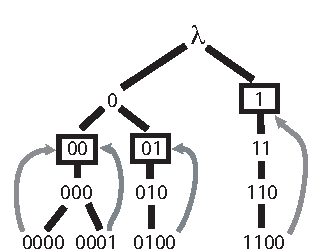
\includegraphics{pics/exthash-tree}
\caption{Reprezentace mno�iny $S$. Vrchol reprezentuj�c� prefix $0$, by ve
sv�m podstrom� m�l 3 prvky, co� je v�ce, ne� po�adujeme pomoc� hodnoty
$b$.}
\label{fig.hash.extern}
\end{figure}

Z obr. \ref{fig.hash.extern} plyne, �e hodnota $d(S) = 2$.
\end{priklad}

\begin{tvrzeni}
Plat�: Kdy� $d(s) = k$ a prvek $t$ m� stejn� prefix d�lky $k$ jako $s$, 
pak $d(s) = d(t)$. 
\end{tvrzeni}

Reprezentace: 
\begin{itemize}
\item adres��: ke ka�d�mu slovu $\alpha$ d�lky $d(S)$ je p�i�azena adresa 
str�nky, kter� obsahuje prvky $s \in S$, �e $h(s)$ m� prefix $\alpha$.
Tato slova d�lky $d(s)$ jsou lexikograficky uspo��d�na.
\item datov� ��st: str�nky s p�i�azen�mi prvky
\end{itemize}

\begin{priklad}
P��klad adres��e pro mno�inu $\{0000, 0001, 0100, 1001 \}$:

\vspace{5mm}

\begin{tabular}{lll}
00 & $\rightarrow$ & 0000, 0001 \\
01 & $\rightarrow$ & 0100 \\
\hline
10 & $\searrow$ & \\
11 & $\rightarrow$ & 1001 \\
\end{tabular}
\end{priklad}

\begin{pozn}
Up�esn�n� reprezentace str�nky (str�nek): \\
Prvek $s \in S$ je ulo�en na str�nce, kter� obsahuje v�echny prvky $t \in
S$ takov�, �e prefix $h(t)$ d�lky $d(s)$ bude je stejn� jako $h(s)$, tato st�nka
bude p�i�azena v�em slov�m $\alpha$ d�lky $d(S)$ takov�m, �e prefix $h(s)$ d�lky
$d(s)$ je prefix $\alpha$. \\
Pokud $\alpha$ neobsahuje ��dn� takov� prefix, tak je mu p�i�azena str�nka
NIL.
\end{pozn}

\subsection{Operace ACCESS}

viz algoritmus \ref{alg:exthash.access}

\begin{algorithm}[!htb]
\caption{ACCESS pro extern� ha�ov�n�}
\label{alg:exthash.access}
ACCESS(x)
\begin{enumerate}
\item Spo��t�me $h(x)$, nat�hneme adres��, nalezneme $d(S)$ a najdeme
str�nky odpov�daj�c� prefixu $h(x)$ d�lky $d(S)$
\item Nat�hneme odpov�daj�c� str�nku do pam�ti, zjist�me, zda obsahuje $x$ a
kdy� ano, provedeme po�adoven� �pravy.
\item Str�nku ulo��me zp�t na stejn� m�sto.
\end{enumerate}
\end{algorithm}

Operace ACCESS vy�aduje 3 p��stupy na extern� medium. (za p�edpokladu, �e
adres�� je tak� ulo�en na extern�m mediu a zab�r� jednu str�nku) 

Pro rychlou implementaci aktualiza�n�ch operac� je vhodn� m�t u ka�d�
str�nky ulo�eno informaci kolik je prvk� na str�nce.


\subsection{Operace INSERT}

viz algoritmus \ref{alg:exthash.insert}

% pozn: \mnote nesmi byt uvnitr prostredi algorithm
\begin{algorithm}[!htb]
\caption{INSERT pro extern� ha�ov�n�}
\label{alg:exthash.insert}
INSERT(x)
\begin{enumerate}
\item Spo��t�me $h(x)$, nat�hneme adres��, nalezneme $d(S)$ a nalezneme adresu
str�nky odpov�daj�c� prefixu $h(x)$ d�lky $d(S)$. (XXX odkud vezmu $d(S)$ ?)
% XXX \mnote{$d(S)$ vezmu odkud ?}
\item Nat�hneme do pam�ti odpov�daj�c� str�nku. kdy� v n� existuje $x$ 
$\rightarrow$ konec
\item Kdy� neobsahuje $x$ a m� m�n� prvk� ne� $b$, vlo��me $x$ do t�to str�nky
a ulo��me ji zp�tky na stejn� m�sto a aktualizujeme adres�� (po�ty prvk�
na str�nce)
\item Kdy� str�nka prvek $x$ neobsahuje a m� $b$ prvk�, str�nku rozd�l�me
(nalezneme nov� $d(s)$ pro $s$ z t�to str�nky i s p�idan�m $x$), str�nky 
ulo��me a aktualizujeme adres��.
\end{enumerate}
\end{algorithm}
\mnote{pokud je nov� nalezen� $d(s) \leq d(S)$, adres�� se zv�t�ovat nebude}

Operace INSERT vy�aduje 6 p��stup� na extern� medium.

\begin{pozn}
Roz�t�pen� str�nky nemus� nutn� znamenat zv�t�en� adres��e.
\end{pozn}

\begin{priklad}
\label{priklad:exthash.insert2}
Do mno�iny z p��kladu \ref{priklad:exthash.tree} vlo��me pomoc� operace
INSERT prvek 1111. Hodnota $d(1100) = 1$ se po vlo�en� prvku 1111
nezm�n�. Podstrom reprezentuj�c� prvky mno�iny $S$ s prefixem 11
bude m�t po vlo�en� prvku 1111 dva syny. (viz obr.
\ref{fig.hash.extern.ins})

\begin{figure}[!htb]
\centering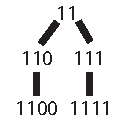
\includegraphics{pics/exthash-ins}
\caption{Podstrom reprezentuj�c� prvky mno�iny $S$ s prefixem 11 po
vlo�en� prvku 1111}
\label{fig.hash.extern.ins}
\end{figure}

Pokud vezmeme situaci danou po vlo�en� prvku 1111, bude adres�� vypadat
takto:

\vspace{5mm}

\begin{tabular}{lll}
00 & $\rightarrow$ & 0000, 0001 \\
\hline
01 & $\rightarrow$ & 0100 \\
\hline
10 & $\searrow$ & 	 \\
  & &  1001 \\
11 & $\nearrow$	& \\
\end{tabular}

\vspace{5mm}

Nyn� vlo��me prvek 0010. V tomto p��pad� dojde ke zv�t�en� adres��e:

\vspace{5mm}

\begin{tabular}{lll}
000 & $\rightarrow$ & 0000, 0001 \\
\hline
001 & $\rightarrow$ & 0010 \\
\hline
010 & $\rightarrow$ & 0100 \\
011 & $\nearrow$ & \\
\hline
100 & $\searrow$ & \\
101 & $\rightarrow$ &  1001, 1111 \\
110 & $\nearrow$ & \\
111 & $\nearrow$ & \\
\end{tabular}

\vspace{5mm}

Hodnota $d(S)$ je nyn� 3.
\end{priklad}


\subsection{Operace DELETE}

viz algoritmus \ref{alg:exthash.delete}

\begin{algorithm}[!htb]
\caption{DELETE pro extern� ha�ov�n�}
\label{alg:exthash.delete}
DELETE(x)
\begin{enumerate}
\item spo��t�me $h(x)$, nat�hneme adres��, nalezneme $d(S)$, nalezneme adresu
str�nky odpov�daj�c� prefixu $h(x)$ d�lky $d(S)$, zjist�me zda po odebr�n�
prvku $x$ m��e nastat spojov�n� str�nek a pokud ano, nalezneme adresu
str�nky, kter� se spoj� s na�� str�nkou
\item nat�hneme odpov�daj�c� str�nku do pam�ti, zjist�me zda obsahuje $x$,
pokud ne, tak konec
\item kdy� obsahuje $x$ a nem��e doj�t ke slou�en� str�nek, tak odstran�me
$x$, str�nku ulo��me na stejn� m�sto a aktualizujeme adres�� (po�ty prvk� na
str�nce)
\item kdy� obsahuje a dojde ke slu�ov�n�, pak odstran�me $x$, nat�hneme
druhou str�nku a str�nky slou��me, ulo��me novou str�nku a aktualizujeme
adres��.
\end{enumerate}
\end{algorithm}
\mnote{pro aktualizaci adres��e to mohou b�t 2 operace - na�ten� a
ulo�en�. z�ejm� proto, aby mohlo b�t sou�asn� pu�t�no v�c operac�.}

\begin{priklad}
Pro situaci z p��kladu \ref{priklad:exthash.insert2} provedeme
DELETE(0100). V adres��i budou pak polo�ky 010 a 011 ukazovat na pr�zdnou
str�nku (NIL). Adres�� z�stal po t�to operaci stejn�.

Nyn� sma�eme prvek 0001.

\begin{figure}[!htb]
\centering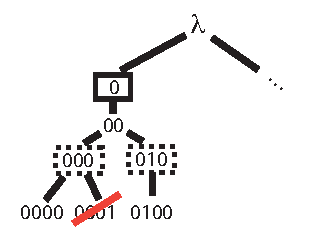
\includegraphics{pics/exthash-del}
\caption{��st stromu reprezentuj�c�ho mno�inu $S$ p�ed smaz�n�m prvku 0001}
\label{fig.hash.extern.del}
\end{figure}

Na obr. \ref{fig.hash.extern.del} je vid�t, �e po smaz�n� prvku 
0001 m��e b�t adres�� op�t zmen�en.

Po proveden� DELETE(0001) bude adres�� vypadat takto:

\vspace{5mm}

\begin{tabular}{lll}
000 & $\rightarrow$ & 0000, 0010 \\
001 & $\nearrow$ & \\
\hline
010 & $\rightarrow$ & NIL \\
011 & $\nearrow$ & \\
\hline
100 & $\searrow$ & \\
101 & $\rightarrow$ &  1001, 1111 \\
110 & $\nearrow$ & \\
111 & $\nearrow$ & \\
\end{tabular}

\vspace{5mm}

Nyn� m��eme prov�st zmen�en� adres��e na:

\vspace{5mm}

\begin{tabular}{lll}
00 & $\rightarrow$ & 0000, 0010 \\
01 & $\nearrow$ & \\
\hline
10 & $\rightarrow$ & 1100, 1111	 \\
11 & $\nearrow$	& \\
\end{tabular}

\vspace{5mm}

Tento adres�� m��eme je�t� zmen�it:

\vspace{5mm}

\begin{tabular}{lll}
0 & $\rightarrow$ & 0000, 0010 \\
\hline
1 & $\rightarrow$ & 1100, 1111 \\
\end{tabular}
\end{priklad}

\begin{pozn}
Pesimistick� odhad pro operaci DELETE je nejv��e 6 p��stup� na extern� 
medium.
\end{pozn}

\subsubsection{Aktualizace adres��e}

V posledn�m kroku DELETE se prov�d� aktualizace adres��e. 
Nejprve provedeme opraven� odkaz� na str�nky: pokud u sud�ho z�znamu v
adres��i dojde k vypr�zdn�n� str�nky, bude tam odkaz na NIL. pokud dojde k
vypr�zdn�n� u lich� str�nky, p�ehod� se odkaz na p�edchoz� (sudou)
str�nku.

Potom se testuje, zda jde adres�� zmen�it. Zmen�ov�n� prov�d�me tak
dlouho, dokud to jde.

\subsection{Reprezentace adres��e}

\begin{itemize}
\item reprezentovat jako posloupnost dvojic (adresa str�nky, po�et prvk� na
str�nce), kde $i$-t� dvojice je p�i�azen� $i$-t�mu slovu v lexikografick�m
uspo��d�n�.
\item zv�t�ov�n� adres��e znamen� zdvojen� prvk�
\item test na zmen�ov�n� adres��e - testujeme, zda adresa na lich�m m�st�
je stejn� jako adresa na n�sleduj�c�m sud�m m�st� - pokud ano, tak zmen��m
adres�� vymaz�n�m sud�ch �len� posloupnosti.
\end{itemize}

O�ek�van� zapln�n� str�nky p�i rovnom�rn�m rozlo�en� dat je 
$b \ln 2 \approx 0.69 b$

O�ek�van� velikost adres��e je $\frac{e}{b \ln 2} n^{1 + \frac{1}{b}}$ (p�i
rovnom�rn�m rozlo�en� dat)

\begin{pozn}
�len $n^{1 + \frac{1}{b}}$ nen� line�rn�, zde je probl�m, proto se to
nehod� pro mal� $b$.
\end{pozn}

\begin{tabular}{|l||l|l|l|l|}
\hline
b/n   	&$10^5$   &$10^6$ 	&$10^8$ 	&$10^{10}$    \\
\hline
2  	&$6.2*10^7$  &$1.96*10^8$	&$1.96*10^{11}$	&$1.96*10^{14}$ \\
10	&$1.2*10^5$  &$1.5*10^6$	&$2.4*10^8$	&$3.9*10^{10}$  \\
50	&$9.8*10^3$  &$1.0*10^6$	&$1.1*10^8$	&$1.2*10^{10}$  \\
100	&$4.4*10^3$  &$4.5*10^4$	&$4.7*10^6$	&$4.9*10^8$   \\
\hline
\end{tabular}

\vspace{5mm}

Jak je vid�t, pro $b = 2$ se to nehod�, adres�� je v�t�� ne� velikost dat.

\begin{pozn}
Kdy� pracujeme s velikost� $S$ kolem $10^{10}$, pak je vhodn�, aby 
$b \geq 100$. Pro v�t�� mno�iny $S$ mus� b�t $b$ v�t��.
\end{pozn}

% --------------------------------------------------------------------------
\section{Perfektn� ha�ov�n�}

Perfektn�m ha�ov�n�m mysl�me �lohu nal�zt pro danou pevnou mno�inu 
$S \subseteq U, |S| = n$ perfektn� ha�ovac� funkci, tj. funkci, kter� nem� na 
mno�in� $S$ kolize. Tato �loha nep�ipou�t� p�irozenou implementaci 
operace INSERT, proto�e p�idan� prvek m��e zp�sobit kolizi. 
Typick� p��klad pou�it� je tabulka kl��ov�ch slov kompil�toru.

\begin{defn}
Funkce $h: U \to \intrange{0}{m-1}$ je perfektn� pro $S$, kdy� je na S
prost� ($\forall x\neq y \in S$ plat� $h(x) \neq h(y)$).
\end{defn}

Za jak�ch podm�nek lze povolit INSERT? Mus� b�t m�lo
pravd�podobn�. Prvky nav�c se d�vaj� jinam a po jist� dob� se v�e
p�epo��t� do jedn� tabulky pro novou perfektn� ha�ovac� funkci.

\begin{samepage}
Po�adavky na hledanou ha�ovac� funkci:
\begin{enumerate}
  \item $h$ je perfektn� na $S$
  \item $\forall x$ je $h(x)$ rychle spo�itateln�
  \item $m$ ��dov� srovnateln� s $n$
  \item zak�dov�n� $h$ vy�aduje m�lo prostoru
\end{enumerate}
\end{samepage}

Po�adavky 2) a 3) jdou proti sob�. A a� se n�m je poda�� skloubit,
budeme m�t probl�my s 4). A nav�c hled�n� $h$ potrv� dlouho.

% ..........................................................................
\subsection{Perfektn� ha�ovac� funkce do tabulky velikosti $n^2$}

Vyu�ijeme, co u� v�me o univerz�ln�m ha�ov�n�. Pro $k \in \intrange{1}{N-1}$ 
a pro pevn� $m$ definujme 
\begin{equation}
h_k(x) = ( kx \bmod N ) \bmod m, \quad\text{kde $N=|U|$ je prvo��slo.}
\end{equation}
Budeme hledat vhodn� $k$, $m$.
Definujme m�ru perfektnosti
\begin{equation}
d = \sum_{k=1}^{N-1} \sum_{x \neq y \in S} \delta_{h_k}(x,y)
\end{equation}
a pro $k \in \intrange{1}{N-1}$ polo�me
\begin{equation}
b_k(i) = |\{ x \in S : h_k(x) = i \}|
\end{equation}

Jednak plat�
\begin{align}
\label{bki2}
% vnitrni suma (s mocninou) dana do zavorky aby byly v poradku priority 
% (from V. Havranek)
d & = \sum_{k=1}^{N-1} \left( ( \sum_{i=0}^{m-1} ( b_k(i) )^2 ) -n \right)\\
\intertext{a tak�}
d & = \sum_{x \neq y \in S} |\{ k : h_k(x)=h_k(y) \}|
	&&\text{prohozen�m sum}\\
\end{align}

Co znamen� $h_k(x) = h_k(y)$ pro $x \neq y$? N�sleduj�c� tvrzen� jsou
ekvivalentn�:
\begin{align*}
kx \bmod N & = ky \bmod N && \pmod m\\
k(x-y) \bmod N & = 0 && \pmod m\\
k(x-y) \bmod N & = r m && \text{pro } r \in 
% *ceil -> *floor (fakticka poznamka od Ladislava Proska
	\{ - \lfloor N/m \rfloor .. \lfloor N/m \rfloor \} - \{0\}, \\
\end{align*}
tedy
\[
d \leq \sum_{x \neq y \in S} 2 \frac Nm = \frac{2 n(n-1) N}m
\]
a dosazen�m do \eqref{bki2}, podle p�ihr�dkov�ho principu
\begin{equation}
\label{existsk}
\exists k : \sum_{i=0}^{m-1} ( b_k(i) )^2 \leq n + \frac{2 n(n-1)}m
\end{equation}

Pro speci�ln� velikosti tabulky dost�v�me dosazen�m do \eqref{existsk}:
\begin{align}
\label{3n}
&\text{Pro } m = n: 
&& \exists k \text{ naleziteln� v �ase }O(nN): 
\sum_{i=0}^{m-1} ( b_k(i) )^2 < 3n\\
\label{perf}
&\text{Pro } m = 1 + n(n-1): 
&& \exists k \text{ naleziteln� v �ase }O(nN):  
h_k \text{ je perfektn�} 
\end{align}

\begin{proof}
Prob�r�me v�echny mo�nosti pro $k$, t�ch je $O(N)$.
\begin{enumerate}
\item[\eqref{3n}]
Pro dan� $k$ spo��t�me $\sum ( b_k(i) )^2$ v �ase $O(n) = O(m)$.
\item[\eqref{perf}]
$\sum ( b_k(i) )^2 \leq n + \frac{2 n(n-1)}{1+ n(n-1)} < n + 2$.
Kdyby $h_k$ nebyla perfektn�, pak 
$\exists j : b_k(j) \geq 2$
a
$\sum ( b_k(i) )^2 \geq (n-2) 1^2 + 1 \cdot 2^2 = n + 2$,
spor.
P�i hled�n� $k$ ov���me perfektnost $h_k$ v �ase $O(n)$.
% zmatek s indexy u k (T. Matousek):
% Tohle by melo byt vporadku. k je jako scitaci index jen v (4.8) a (4.10)
% a dal uz ne.
% Ten soucet v d jde pres vsechny hashovaci funkce a jedna z nich je ta
% prava. Ja bych to tak nechal, je to ok. Staci smazat tu *.
\end{enumerate}
\end{proof}

Nyn� m�me perfektn� ha�ovac� funkci, kter� ale poru�uje po�adavek (3).
% ..........................................................................
\subsection{Perfektn� ha�ovac� funkce do tabulky velikosti $3n$}

Zkombinujeme oba v�sledky z p�edchoz� ��sti.
% --- nejprve prvn� funkc� ha�ujeme do tabulky velikosti $< 3n$

Podle \eqref{3n} nalezneme $k$ takov�, �e
$\sum ( b_k(i) )^2 < 3n$.

Pro ka�d� $i \in \intrange{0}{n-1}$ vezmeme mno�inu koliduj�c�ch prvk�
$S_i = \{ s \in S : h_k(s) = i \}$.
Ozna�me $n_i = |S_i|$.

Podle \eqref{perf} pro ka�d� $i$ nalezneme $k_i$ takov�, �e
pro $m_i = 1 + n_i(n_i-1)$ je $h_{k_i}$ perfektn� pro $S_i$.

Ka�dou zaha�ovanou mno�inu $S_i$ ulo��me ve v�sledn� tabulce od pozice
$d_i$: 
\[
d_i = \sum_{j=0}^{i-1}(1 + n_j(n_j-1)).
\]

Kone�n� definujme
\[
g(x) = d_i + h_{k_i}(x),\quad\text{kde } i = h_k(x),
\]
kter� je perfektn� a velikost tabulky je
\[
m = d_n = \sum_{j=0}^{n-1}(1 + n_j(n_j-1))
\leq \sum_{j=0}^{n-1} n_j^2
=  \sum_{j=0}^{n-1} (b_k(j))^2
< 3n
\]

Ov�em na zak�dov�n� t�to funkce pot�ebujeme hodn� pam�ti: 
nevad� n�m $d_i$, 
ale $k$ a ka�d� $k_i$ je velikosti $O(N)$, 
tedy pot�ebujeme $n \log_2 N$ bit�, co� odporuje na�emu po�adavku (4).
V dal��ch kroc�ch budeme zmen�ovat ��sla definuj�c� ha�ovac� funkci.
% ..........................................................................
\subsubsection{Podobn� funkce dan� ��slem velikosti $O(N)$}

\mnote{lep�� jm�na prom�nn�ch!}
Zvolme prvo��slo $p_1$ takov�, �e 
$1 +n(n-1) \leq p_1 \leq 1+ 2n(n-1)$. N�jak� takov� mus� existovat
(Bertrand�v postul�t: $\forall n>1 \exists$ prov��slo p, �e 
$n < p < 2n$).
Podle \eqref{perf} %TODO, mus�me dok�zat m \geq, co� m�rn� zatemn� dk.
$\exists k : h_k(x) = ( kx \bmod N) \bmod p_1$ 
je perfektn� na $S$.

Vytvo�me
\[
S_1 = \{ h_k(s) : s \in S\} \subset \intrange{0}{p_1 -1}
\]
a na $S_1$ aplikujme p�edchoz� sekci, kde $N = p_1$.

Dost�v�me ha�ovac� funkci $g_1$, kter�
\begin{itemize}
\item je perfektn� pro $S$
\item je spo�itateln� v �ase $O(1)$ 
\item ha�uje do tabulky $<3n$ 
\item je ur�ena 1 ��slem velikosti $O(N)$ \\
 \quad a $O(n)$ ��sly velikosti $O(n^2)$ 
\end{itemize}

% ..........................................................................
\subsubsection{Podobn� funkce dan� ��slem velikosti $O(n^2\log N)$}
Pro extr�mn� p��pady typu $N = 2^{10^6}$ je�t� postup vylep��me,
��m� zmen��me velikost ��sel k�duj�c�ch perfektn� ha�ovac� funkci 
na $O(\log N)$.

\begin{lemma}
\label{n2logN}
Pro ka�dou mno�inu $S \subseteq \intrange{0}{N-1}$ velikosti $n$ existuje
prvo��slo $p$ takov�, �e $f_{p}(x) = x \bmod p$ je perfektn� na
$S$ a $p = O(n^2 \log N)$.
\end{lemma}

Vyu�it�: pro $S$ najdeme prvo��slo $p_0$ velikosti $O(n^2 \log N)$
takov�, �e $f_{p_0}$ je perfektn� na $S$. Vytvo��me 
\[
S_0 = \{ f_{p_0}(s) : s \in S\} \subset \intrange{0}{p_0-1}
\]
a na $S_0$ aplikujme p�edchoz� postup, kde $N = p_0$.

Tedy pro ka�dou mno�inu $S$ velikosti $n$ existuje ha�ovac� funkce $f$, kter�
\begin{itemize}
\item je perfektn� pro $S$
\item je spo�itateln� v �ase $O(1)$ 
\item ha�uje do tabulky $<3n$ 
\item je ur�ena 2 ��sly velikosti $O(n^2 \log N)$ \\
 \quad a $O(n)$ ��sly velikosti $O(n^2)$ 
\end{itemize}

\begin{lemma}
\label{prvociselnidelitele}
Nech� $r$ je ��slo a $p_1, \ldots, p_q$ jsou v�echny jeho prvo��seln�
d�litele. Pak $q=O(\log r / \log\log r)$.
\end{lemma}
\begin{proof}
\begin{align*}
r & \geq \prod_{i=1}^q p_i\\
 & > q! \\
 & = \exp(\sum_{i=1}^q \ln i) \\
 & > \exp(\int_1^q \ln x \,dx) \\
 & \geq {\left( \frac qe \right)}^q \qquad\text{kde } \exp(x)=e^x
\end{align*}
Tedy
\mnote{skok}
\[
q \leq c \frac{\ln r}{\ln\ln r} \quad\text{pro vhodnou konstantu $c$.}
\]
\end{proof}
\begin{proof}[D�kaz lemmatu \ref{n2logN}]
P�edpokl�dejme $S = \{ x_1 < \ldots < x_n \}$.
Ha�ovac� funkce $f_t(x) = x \bmod t$ je perfektn� pr�v� kdy� $t$ je
nesoud�ln� s ��slem
\[
D = \prod_{i>j} (x_i - x_j) < N^{n^2}
\]
Podle \ref{prvociselnidelitele} je mezi prvn�mi $(c \ln D / \ln\ln D)+1$
prvo��sly alespo� jedno, kter� ned�l� $D$. V�me, �e $p_k = O(k \ln
k)$, tedy 
$(c \ln D / \ln\ln D) +1$-n� prvo��slo m� velikost
$O(\ln D) = O( n^2 \ln N)$.
\end{proof}
\mnote{nalezeni prvocisla $p_0$ vyzaduje cas $O(n^2\log N)$.}

% ..........................................................................
\subsection{GPERF}

Jin� konstrukce perfektn� ha�ovac� funkce je pou�ita v programu
{\tt gperf}. Distribuov�n pod GPL. 
Jeho n�vrh je pops�n v \cite{douglas-GPERF}.


% --------------------------------------------------------------------------
\def\xx{% commented out
\section{Ha�ov�n� pro extern� pam�}

\mnote{Tohle u� Koubek nep�edn��} % - zrejme komentar od M.Vidnera
% - sice to Koubek neprednasi (prednasi se to v predmetu OZD), 
% ale u statnic se to zkousi
% Externi hashovani je popsano v jine sekci.
Adres��.

MEMBER, INSERT, DELETE

O�ek�van� zapln�n� str�nky, po�et str�nek, velikost adres��e --- jen
citace, tabulka pro n�kter� ��sla.
}% commented out

% ==========================================================================
% Sou��st skript na Datov� struktury. Viz main.tex
\markright{$ $Id$ $}

\chapter{Trie}

\emph{Trie}\footnote{N�zev \emph{trie} poch�z� z anglick�ho 
"re{\bf trie}val", tedy vyzvednut�. N�zory na to, jak vyslovovat 
"trie" se r�zn�. V �e�tin� se zpravidla vyslovuje tak jak se p��e.} 
je rovinn� implementace slovn�ku.

M�me abecedu $\Sigma$ velikosti $k$. Universum jsou v�echna slova nad
$\Sigma$ d�lky pr�v� $l$ (nekone�nou mno�inu si nem��eme dovolit a
krat�� slova dopln�me zprava mezerami). Chceme reprezentovat mno�inu
slov $S \subseteq U$.


% --------------------------------------------------------------------------

\section{Z�kladn� varianta}

\begin{defn}
\emph{Trie} nad $\Sigma$ je kone�n� strom, jeho� ka�d� vnit�n�
vrchol m� pr�v� $k$ syn�, kter� jsou jednozna�n� ohodnoceny prvky $\Sigma$.
Ka�d�mu vnit�n�mu vrcholu trie odpov�d� slovo nad $\Sigma$ d�lky
nejv��e $l$: ko�enu
odpov�d� pr�zdn� slovo $\Lambda$; kdy� vrcholu $v$ odpov�d� slovo
$\alpha$, pak $v[a]$, synu $v$ ohodnocen�mu p�smenem $a$, odpov�d�
slovo $\alpha a$.
\end{defn}

\newcommand{\Nal}{\textrm{Nal}}
\begin{defn}
�ekneme, �e trie nad $\Sigma$ \emph{reprezentuje mno�inu} $S$, kdy�:
\begin{itemize}
  \item List�m je p�i�azena boolovsk� funkce n�le�en� \Nal: $\Nal(t)$ je
  	true pr�v� kdy� slovo, kter� odpov�d� listu $t$, je v $S$.
  \item (\emph{prefixov� podm�nka}) Kdy� $v$ je vnit�n� vrchol trie 
	odpov�daj�c� slovu $\alpha$, pak
  	existuje $\beta \in S$ takov�, �e $\alpha$ je prefix $\beta$.
  \item Pro ka�d� slovo $\alpha \in S$ existuje v trie list odpov�daj�c�
  	$\alpha$.
\end{itemize}
\end{defn}

% podle http://en.wikipedia.org/wiki/Trie
\begin{pozn}
Na rozd�l od bin�rn�ho vyhled�vac�ho stromu (viz kapitola~\ref{bvs},
sekce~\ref{bvs:obecne}), ��dn� vrchol ve strom� neobsahuje ulo�en� kl��,
kter� reprezentuje. Nam�sto toho jeho pozice ve strom� ud�v� kl��, kter�
reprezentuje\footnote{Tato a n�sleduj�c� pozn�mka jsou voln� p�evzaty z
encyklopedie Wikipedia, heslo Trie.}. 
Pouze n�kter� vrcholy ve strom� obsahuj� data - nap�. pro
implementaci slovn�ku s hesly by data ulo�en� v listech obsahovala popis
tohoho hesla\footnote{Nap�. slovn�k spisovatel�, kde listy ve trie by
odpov�daly jm�n�m jednotliv�ch spisovatel� a data ulo�en� v nich by 
obsahovala seznam jejich d�l.}.
\end{pozn}

% podle http://en.wikipedia.org/wiki/Trie
\begin{pozn}
Pro� jsou trie v�hodn� ?

\begin{itemize}
  \item Vyhled�v�n� kl��� je rychlej�� ne� v BVS. Vyhled�n� kl��e d�lky
  $m$ vy�aduje pouze $O(m)$ �asu. Pro BVS je to $O(m^2)$ v nejhor��m p��pad�,
  proto�e se mus� opakovan� porovn�vat po��te�n� znaky hledan�ho slova.
  Dal�� v�hoda je pou�it� indexace pomoc� znak� v operaci MEMBER.
  \item Trie zab�raj� m�n� m�sta. Proto�e nejsou kl��e v trie ulo�eny
  explicitn�, pro ulo�en� jednoho kl��e je pot�eba pouze amortizovan�
  konstantn� prostor.
  \item Pomoc� trie lze jednodu�e prov�d�t operaci hled�n� nejdel��ho 
  prefixu\footnote{anglicky ``longest-prefix matching``}, kde pot�ebujeme
  naj�t kl��, kter� m� nejdel�� shodn� prefix s hledan�m
  kl��em\footnote{To se hod� nap��klad pro implementace s��ov�ch
  opera�n�ch syst�m�, kde je pot�eba prov�d�t tuto operaci pro
  hled�n� v routovac�ch tabulk�ch nebo tabulk�ch pro p�eklad adres. 
  V p��pad� sm�rovac�ch tabulek se pos�l� paket na dal�� "hop" podle 
  c�lov� adresy. Routovac� tabulka obsahuje z�znamy, kter� ud�vaj� adresu
  s�t� a adresu za��zen�, na kter� pos�lat pakety pro tuto s�� - tzv.
  "hop". Tento "hop" se vyb�r� tak, aby c�lov� adresa paketu m�la
  co mo�n� nejdel�� shodn� prefix s n�jakou adresou s�t� v routovac�
  tabulce.}. 
  D�le trie dovoluj� asociovat jednu hodnotu s mno�inou kl���, kter� maj�
  shodn� prefix\footnote{T�m, �e ulo��me data do vnit�n�ch uzl� trie.}.
\end{itemize}
\end{pozn}

% ..........................................................................
\subsection{Algoritmus MEMBER}

viz algoritmus \ref{alg:trie.member}.

\begin{algorithm}[!htb]
\caption{MEMBER pro z�kladn� verzi trie}
\label{alg:trie.member}
\begin{algorithmic}
\STATE \COMMENT {vyhled�n� $x = x_1 \dots x_l$}
\STATE $t := \text{ko�en}$
\STATE $i := 1$
\WHILE {$t \text{ nen� list}$}
        \STATE $t := t[x_i]$ // sestup podle znaku $x_i$
        \STATE $i := i + 1$
\ENDWHILE
\STATE \COMMENT {test}
\STATE \textbf{return} $\Nal(t)$
\end{algorithmic}
\end{algorithm}

Na tomto algoritmu je zaj�mav� to, �e pou��v� jednotliv� znaky hledan�ho
slova $x$ k indexaci v jednotliv�ch vrcholech trie (viz ��dek s
koment��em ve v�pisu algoritmu~\ref{alg:trie.member}.). To dovoluje naj�t
vrchol do kter�ho se m� p�i hled�n� sestoupit v �ase $O(1)$. Tedy
slo�itost operace MEMBER je $O(l)$, proto�e mus�me proj�t nejv��e $l$
vrchol� ne� dos�hneme listu (d�lka slov je nejv��e $l$).

% ..........................................................................
\subsection{Algoritmus INSERT}

viz algoritmus \ref{alg:trie.insert}.

\begin{algorithm}[!htb]
\caption{INSERT pro z�kladn� verzi trie}
\label{alg:trie.insert}
\begin{algorithmic}
\STATE \COMMENT {vyhledej $x$ pomoc� operace MEMBER(x)}
\IF[trie nemus� b�t tak hlubok�, jak pot�ebujeme] {\textbf{not} $\Nal(t)$}
        \WHILE {$i \leq l$}
                \STATE vrcholu $t$ p�idej $k$ list� ohodnocen�ch
                p�smeny z $\Sigma$, jejich $\Nal := \textit{false}$
                \STATE $t := t[x_i]$
                \STATE $i := i + 1$
        \ENDWHILE
        \STATE $\Nal(t) := \textit{true}$
\ENDIF
\end{algorithmic}
\end{algorithm}

P�i operaci INSERT se sestupuje a� na �rove� d�lky slova, p�i�em� se
p�id�vaj� nov� �rovn� v p��pad� �e nejsou v trie p��tomny\footnote{Celkem 
hezky si lze proces p�id�v�n� nov�ch hladin v r�mci jedn� v�tve p�edstavit 
tak, �e v ka�d� hladin�, kter� je nov� p�idan�, "vyroste smet�k" s $k$ 
vrcholy.}.

% ..........................................................................
\subsection{Algoritmus DELETE}

viz algoritmus \ref{alg:trie.delete}.

\begin{algorithm}[!htb]
\caption{DELETE pro z�kladn� verzi trie}
\label{alg:trie.delete}
\begin{algorithmic}
\STATE \COMMENT {vyhledej $x$ pomoc� operace MEMBER(x)}
\IF {$\Nal(t)$}
        \STATE $\Nal(t) := \textit{false}$
        \STATE $t := \text{otec } t$
        \STATE \COMMENT {oprav�me prefixovou podm�nku}
        \WHILE {v�ichni synov� $t$ jsou listy s $\Nal = \textit{false}$}
                \STATE zru� listy $t$
                \STATE $\Nal(t) := \textit{false}$
                \STATE $t := \text{otec } t$
        \ENDWHILE
\ENDIF  
\end{algorithmic}
\end{algorithm}

Analogicky k operaci INSERT doch�z� k ru�en� hladin v r�mci jedn� v�tve
v p��pad� �e v�echny
listy v hladin� maj� hodnotu $\Nal = \textit{false}$.

Pou�ili jsme obrat $t := \text{otec } t$. To lze prov�st bu� tak, �e
se vrchol krom� sv�ch syn� odkazuje i na sv�ho otce a spot�ebuje tak
pam� nav�c, nebo se cesta z ko�ene do aktu�ln�ho vrcholu b�hem
sestupu ve stromu pamatuje na z�sobn�ku. Tento trik se pou��v� u 
v�ech stromov�ch struktur.

% ..........................................................................
\subsection{�asov� a pam�ov� slo�itost}

Jedna iterace cyklu zabere konstantn� �as. �as pro MEMBER je $O(l)$,
�as pro INSERT a DELETE je $O(l k)$. Pam�ov� slo�itost trie v nejhor��m
p��pad� je po�et
ulo�en�ch slov n�soben� d�lkou cesty a po�tem syn�, tedy $O(|S| l k)$.

\begin{pozn}
V p��pad�, kdy S obsahuje (skoro) v�echna slova d�lky $l$, tak m��e
m�t slo�itost jen $O(|S|)$.
\end{pozn}

% --------------------------------------------------------------------------
\section{Komprimovan� trie}

M�jme $\Sigma = \{0,1,2\}$, $l=7$.
$S = \{0202011, 0202012, 0202021, 1212102, 1212111, 1212121, 1212122\}$.
Nekomprimovan� trie pro tuto mno�inu je na obr�zku \ref{fig:tries}.
Vid�me, �e p�smena na druh� a� p�t� pozici jsou v�dy stejn� a
% XXX \uv{prokousat} 
p�edchoz� algoritmy se jimi mus� prokousat. P�esn�ji 
�e�eno, prohl��en� vrcholu $v$, kter� m� jedin�ho 
syna, kter� nen� list s hodnotou $\Nal = \textit{false}$, nep�in�� 
��dnou kladnou informaci, proto�e mno�iny prvk� z $S$, 
kter� jsou reprezentov�ny vrcholy v podstromu otce $v$ a v podstromu 
vrcholu $v$ jsou stejn�. To vedlo k idei tyto vrcholy ze stromu vynechat a
t�m zmen�it (komprimovat) trie.  

\begin{figure}
\centering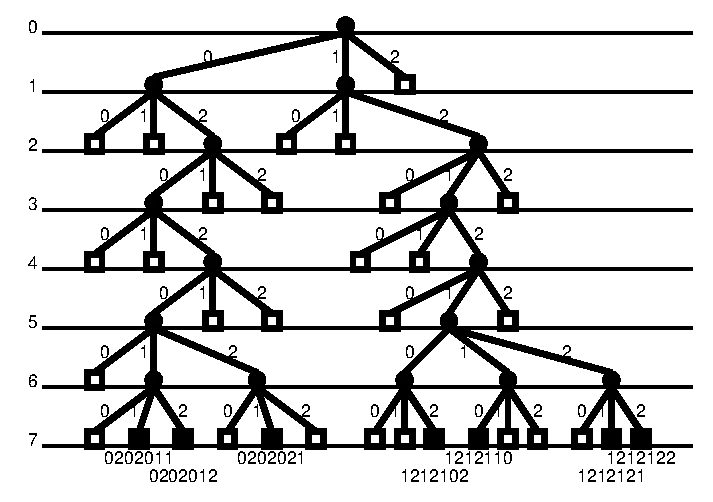
\includegraphics{pics/tries}
\caption{Nekomprimovan� trie. �ern� vypln�n� �tverce zn�zo�uj� listy,
kter� odpov�adj� n�jak�mu slovu z (reprezentovan�) mno�iny $S$. Tyto listy
maj� hodnotu funkce Nal \textit{true}. B�le vypln�n� �tverce ��dn�mu slovu
ze $S$ neodpov�daj�, maj� tedy hodnotu Nal \textit{false}.}
\label{fig:tries}
\end{figure}

\newcommand{\uro}{\textrm{uroven}}
Ke ka�d�mu vrcholu $v$ p�id�me funkci $\uro(v)$ vyjad�uj�c� ��slo �rovn�,
ve kter� se $v$ nach�z� v p�vodn�m trie.
\newcommand{\slo}{\textrm{slovo}}
Ke ka�d�mu listu $v$ p�id�me funkci $\slo(v)$ --- slovo, kter� odpov�d� $v$.

Nyn� m��eme vynech�vat vrcholy podle n�sleduj�c�ho krit�ria: 
je-li $v$ vnit�n� vrchol a v�ichni jeho synov� krom� $w$ jsou listy s
$\Nal = \textit{false}$, pak $v$ vynech a za�a� $w$ na jeho m�sto. Tento proces 
opakujeme dokud trie obsahuje n�jak� vnit�n� vrchol, jeho� v�ichni synov� 
s v�jimkou jednoho jsou listy, pro n� $\Nal = \textit{false}$. 
V�imn�te si, �e ka�d� vnit�n� vrchol m� pr�v� $k$ syn�, kter� jsou 
v jednozna�n� korespondenci s p�smeny abecedy $\Sigma$.

\begin{priklad}
Nech� $\Sigma = \{0,1,2\}$, $l=3$.
$S = \{ 001,102,010,211,212 \}$.

Nekomprimovan� trie pro mno�inu $S$ a jeho komprimovan� varianta je na
obr. \ref{fig:tries.compr1}.

\begin{figure}
\centering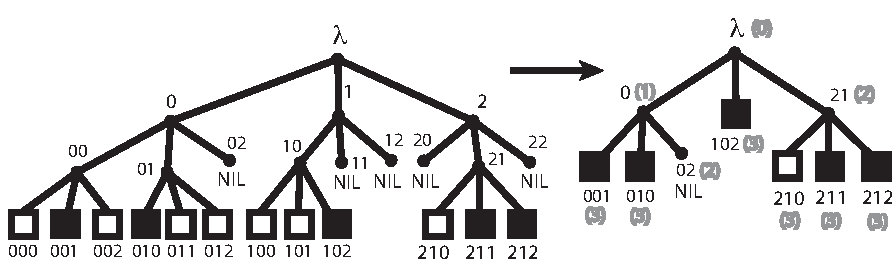
\includegraphics{pics/trie-compr1}
\caption{Komprimace trie. �ed� ��sla v z�vorce zna�� hodnotu $uroven()$}
\label{fig:tries.compr1}
\end{figure}

\end{priklad}


\begin{pozn}
\mnote{Koubek 2002/2003}
Komprimovan� trie je tvo�en� mno�inou vrchol�, kde pro $\beta$ je
$hladina(\beta) = |\beta|$ a otec $\beta$ je nejv�t�� vlastn� prefix,
kter� pat�� do trie + p�idan� listy. Listy jsou prvky z S + slova $\beta
a$, kde $\beta \in$ trie a $\beta a$ nen� prefixem ��dn�ho slova v $S$. 
Pro prvky z $S$ je Nal = True, jinak false. 
Plat� $prvek(\gamma) = \gamma$ pro ka�d� list.

Kdy� $\beta \in$ trie a $a \in \Sigma \rightarrow$
$\Bigl\{$
\begin{tabular}{ll}
$\beta a$ list, & je $a$-t�m synem $\beta$ \\
$\exists \delta \in S$, & �e $\beta a$ je prefixem $\delta$
\end{tabular}

Potom $a$-t� syn $\beta$ je nejkrat�� prefix v mno�in� trie v $S$, kter�
obsahuje $\beta a$.
\end{pozn}

% ..........................................................................
\subsection{MEMBER}

Viz algoritmus \ref{alg:trie.k.mem}

\begin{algorithm}[!htb]
\caption{MEMBER pro komprimovan� trie}
\label{alg:trie.k.mem}
\begin{algorithmic}
\STATE \COMMENT {vyhled�n� $x = x_1 \ldots x_l$}
\STATE $t := \text{ko�en}$
\WHILE {$t \text{ nen� list}$}
        \STATE $i := \uro(t) + 1$
        \STATE $t := t[x_i]$ // $x_i$-t� list
\ENDWHILE
\STATE \COMMENT {test}
\STATE \textbf{return} $\Nal(t) \land \slo(t) = x$
\end{algorithmic}
\end{algorithm}

% XXX zde \mnote{n�co chyb�}

% ..........................................................................
\subsection{INSERT}

Viz algoritmus \ref{alg:trie.k.ins}

\begin{algorithm}
\caption{INSERT pro komprimovan� trie}
\label{alg:trie.k.ins}
\begin{algorithmic}
\STATE \COMMENT {vyhledej $x$}
\IF {$\Nal(t) \land \slo(t) = x$}
	\STATE \COMMENT {Trie u� obsahuje $x$, ned�lej nic.}
\ELSE
        \IF {$\slo(t) = x$}
		\STATE \COMMENT {Trie obsahuje spr�vn� list,
		pouze nastav p��znak. Nap�. "0202010"}
                \STATE $\Nal(t) := \textit{true}$
	\ELSE
		\STATE \COMMENT {Bude pot�eba vlo�it nov� list.}
		\STATE \COMMENT {Najdi, kam ho p�ipojit.}
                \STATE $\alpha$ := nejdel�� spole�n� prefix slov
		$x$ a $\slo(t)$. D�lku $\alpha$ ozna�me $|\alpha|$.
                \STATE $v$ := vrchol na cest� z ko�ene do $t$ takov�,
                �e $\uro(v)$ je nejv�t��, kter� je $\leq |\alpha|$
                \IF {$\uro(v) = |\alpha|$}
                        \STATE \COMMENT {$v$ je otec nov�ho listu}
		\ELSE[$\uro(v) < |\alpha|$]
                        \STATE \COMMENT {Bude pot�eba vytvo�it
			otce nov�ho listu}
                        \STATE $a$ := $\uro(v)+1$-n� p�smeno $\alpha$
                        \STATE $u := v[a]$
                        \STATE \COMMENT {Mezi $v$ a $u$ vytvo� nov�
			vnit�n� vrchol odpov�daj�c� slovu $\alpha$}
                        \STATE $w$ := nov� vrchol, $\uro(w) := |\alpha|$
                        \STATE $v[a] := w$
                        \STATE $c$ := $|\alpha|+1$-n� p�smeno $\slo(t)$
                        \STATE $w[c] := u$
                        \FORALL {$b \in \Sigma, b \neq c$}
                             \STATE $z$ := nov� vrchol, $\uro(z) := |\alpha|+1, \Nal(z) := \textit{false}, \slo(z) := \alpha b$, 
                             \STATE $w[b] := z$
                        \ENDFOR
                        \STATE $v := w$
                \ENDIF
		\STATE \COMMENT {Spr�vn�mu listu p�i�a� $x$}
		\STATE $d$ := $|\alpha|+1$-n� p�smeno $x$
                \STATE $s := v[d]$
                \STATE $\uro(s) := l, \Nal(s) := \textit{true}, \slo(s) := x$
        \ENDIF
\ENDIF
\end{algorithmic}
\end{algorithm}

% ..........................................................................
\subsection{DELETE}

Viz algoritmus \ref{alg:trie.k.del}

\begin{algorithm}[!htb]
\caption{DELETE pro komprimovan� trie}
\label{alg:trie.k.del}
\begin{algorithmic}
\STATE \COMMENT {vyhledej $x$}
\IF {$\Nal(t) \land \slo(t) = x$}
        \STATE $u$ := otec $t$
        \STATE $i := \uro(u)$
        \STATE $\Nal(t) := \textit{false}$
        \STATE $\uro(t) := i+1$, $\slo(t)$ := prefix slova $x$ d�lky $i+1$
        \STATE \COMMENT {vrchol $u$ m� alespo� jednoho syna, kter� nen� list s $\Nal = \textit{false}$}
        \IF {v�ichni synov� $u$ krom� syna $w$ jsou listy s $\Nal = \textit{false}$}
                \STATE $v$ := otec $u$
                \STATE sma� $u$ a v�echny syny $u$ krom� $w$
                \STATE $j := \uro(v) + 1$
                \STATE $v[x_j] := w$ // $x_j$-t� syn $v$ je $w$
        \ENDIF
\ENDIF  
\end{algorithmic}
\end{algorithm}

% ..........................................................................
\subsection{�asov� a pam�ov� slo�itost}

Pam�ov� slo�itost takto komprimovan�ch trie je $O(nk)$, kde 
% oprava by Ladislav Prosek O(nl + kl) -> O(nk)
$n$ je velikost reprezentovan� mno�iny. (maxim�ln� $n-1$ vnit�n�ch vrchol�,
ka�d� s polem d�lky $k$).
�asov� slo�itost operace MEMBER je v nejhor��m
p��pad� $O(l)$, pro INSERT a DELETE je to $O(l+k)$. 
(m��e b�t nutn� p�idat/odebrat jeden vnit�n� vrchol).
% oprava slozitosti v nejhorsim pripade by Ladislav Prosek 

V pr�m�rn�m p��pad� (za p�edpokladu rovnom�rn�ho
rozlo�en� vstupn�ch dat) je to o�ek�van� hloubka trie. Tu
te� spo��t�me.

Nech�
\[
q_d = \pr(\text{trie m� hloubku alespo� $d$})
\]
O�ek�van� hloubka trie reprezentuj�c� $n$ slov je
\[
E_n = \sum_{d=0}^\infty d (q_d - q_{d+1}) = \sum_{d=0}^\infty q_d
\]
Kdy� funkce $\text{pref}_{d-1}$, p�i�azuj�c� slovu 
$\alpha$ jeho prefix d�lky $d-1$, je na mno�in� $S$ prost�,
pak trie reprezentuj�c� mno�inu $S$ m� hloubku nejv��e $d$.
Spo��t�me po�et mno�in o velikosti $n$, na nich� je funkce $\text{pref}_{d-1}$ 
prost�. Tyto mno�iny z�sk�me tak, �e vybereme $n$ prefix� d�lky $d-1$
a ka�d� dopln�me v�emi sufixy d�lky $l-d+1$. Proto t�chto mno�in je
\[
\binom{k^{d-1}}{n} k^{n (l-d+1)}.
\]
Proto�e v�ech podmno�in velikosti $n$ je $\binom{k^l}{n}$ dost�v�me, �e 
\begin{align*}  
q_d 
 &\leq 1 - \frac{\binom{k^{d-1}}{n} k^{n (l-d+1)}}{\binom{k^l}{n}} 
\Biggl\} \text{pravd�podobnost} \\
 &\leq 1 - \frac{k^{d-1}(k^{d-1}-1)\dots(k^{d-1}-(n-1)) k^{n(l-d+1)}}{k^{ln}}\\
 &   = 1 - \prod_{i=0}^{n-1} \left( 1 - \frac{i}{k^{d-1}} \right) \\
 &\leq 1 - \exp\left( \frac{-n^2}{k^{d-1}} \right)\\
 &\leq \frac{n^2}{k^{d-1}},
\end{align*}
pon�vad�
\begin{align*}
                  \prod_{i=0}^{n-1}    \left( 1 - \frac{i}{k^{d-1}} \right)
 &   = \exp\left( \sum_{i=0}^{n-1} \ln \left( 1 - \frac{i}{k^{d-1}} \right)
	   \right)\\
 &\geq \exp\left(         \int_0^n \ln \left( 1 - \frac{i}{k^{d-1}} \right)
	   \right)\\
 &   = \exp\left( \frac{-n^2}{k^{d-1}} \right),
\end{align*} 
(u�ijte integr�ln� kriterium a substituci $x = k^{d-1}(1-t)$) a 
$e^x - 1 \geq x$ (odtud $1 - e^x \leq -x$). 
Tedy pro $c = 2\lceil \log_kn\rceil$ dost�v�me

\begin{align*}
E_n
 & = \sum_{d=1}^cq_d + \sum_{d=c+1}^{\infty}q_d\\
 &\leq c + \sum_{d=c}^{\infty}\frac{n^2}{k^d}\\
 &\leq 2\lceil\log_kn\rceil +
		\left( \frac{n^2}{k^c} \right) \sum_{d=0}^{\infty} k^{-d}\\
 &\leq 2\lceil\log_kn\rceil + \frac{1}{1-1/k}\\
 & = 2\lceil\log_kn\rceil + \frac{k}{k-1}.
\end{align*}

Tedy o�ek�van� �as operace MEMBER je $O(\log_k(n))$ ($O(\frac{\log n}{\log
k})$)
a $O(\log_k(n) + k)$ pro INSERT a DELETE
\mnote{L.Pro�ek: Mo�n� v t� o�ek�van� slo�itosti by �lo +k zanedbat, ale
ne na z�klad� toho tvrzen�, kter� dokazuje jen o�ek�vanou hloubku}
pro komprimovan� trie (za p�edpoklad� rovnom�rn�ho rozlo�en� vstupn�ch dat) 
Zde parametr $k$ vyjad�uje vztah mezi prostorov�mi 
a �asov�mi n�roky.

% . . . .. . . .. .. .. . .  . .. .. .. . . ..  ..  .... . . .. . .. . .
% nasledujici sekci (jeste kompr. trie atd.) dopsal Vladimir Kotal, 2003

\begin{algorithm}[!htb]
	\caption{INSERT pro komprimovan� trie, analogie \ref{alg:trie.k.ins} (verze Koubek 2002)}
\label{alg:trie.k.ins_unk}
\begin{algorithmic}
\STATE INSERT($x=x_1, ..., x_l$)
\STATE $t$ $\leftarrow$ ko�en
\WHILE {$t$ neni list}
  \STATE i $\leftarrow$ hladina($t$), $t$ $\leftarrow$ $(a_{i+1})$-n� syn $t$
\ENDWHILE
\IF {prvek($t$) neni prefix $x$}
  \STATE $\beta$ = nejv�t�� spole�n� prefix $x$ a prvek(t)
  \STATE $\beta a$ = prefix $\alpha$
  \STATE $\beta b$ = prefix prvek($t$)
  \STATE while $hladina(t) > |beta|$ do t $\leftarrow$ otec(t) done
  \IF {$hladina(t) < |\beta|$}
    \STATE vytvo��me nov� vrchol $w$, jeho� synov�, krom� $b$-t�ho syna budou listy s
    \STATE funkcemi Nal = false
    \STATE $prvek(t) = \beta$ + oznaceni syna
    \STATE $hladina(w) = |\beta|, \beta = (a_1, ..., a_i)$
    \STATE necht $v = a_{hladina(t) + 1}$ - t� syn t, b-t� syn w je v
    \STATE $w = a_{hladina(t)+1}$-t� syn t
  \ENDIF
  \STATE z $\leftarrow$ a-t� syn $t$, Nal($z$) = true, prvek($z$) = $x$
\ELSE
  \STATE Nal(t) = true, prvek(t) = $x$
\ENDIF
\end{algorithmic}
\end{algorithm}


\mnote{XXX dalsi neznamy algoritmus z prednasky 2002}
\begin{algorithm}[!htb]
\caption{DELETE pro komprimovan� trie (?)}
\label{alg:trie.k.del_unk}
DELETE($x=x_1, ..., x_l$)
\begin{algorithmic}
\STATE t $\leftarrow$ ko�en
\WHILE {t neni list}
  \STATE i $\leftarrow$ hladina(t), t $\leftarrow$ $(a_{i+1}$-ni syn t
\ENDWHILE
\IF {Nal(t) = true a prvek(t) = j} 
  \STATE Nal(t) = false
  \STATE v $\leftarrow$ otec(t)
  \STATE prvek(t) $\leftarrow$ prefix prvek(t) o d�lce hladina v+1
  \IF {vsichni synove vrchovlu v az na jednoho jsou listy s Nal = false}
    \STATE w $\leftarrow$ syn(v), ktery je bud list s Nal(w) = true nebo neni list
    \STATE necht v je a-t� ($a_i$-ty ???) syn sv�ho otce, v sma�eme a sma�eme
    \STATE v�echny syny $v \neq w$
    \STATE w $\leftarrow$ a-t� ($a_i$-t� ???) syn otce v
  \ENDIF
\ENDIF
\end{algorithmic}
\end{algorithm}


\section{Je�t� komprimovan�j�� trie}

% XXX dopsat !
\begin{priklad}
\label{example.trie.yetmorecompr}

\begin{figure}[!htb]
\centering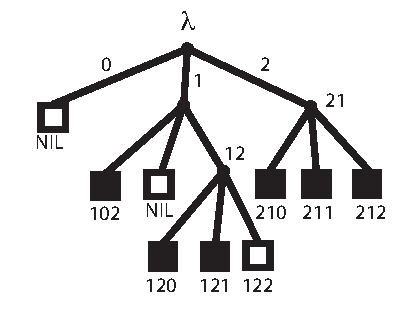
\includegraphics{pics/trie-compr2}
\caption{Nekomprimovan� trie pro p��klad \ref{example.trie.yetmorecompr}}
\label{fig.trie.compr}
\end{figure}

M�jme komprimovan� trie z obr. \ref{fig.trie.compr}
a jeho matici: 

\hspace{5mm}

\begin{tabular}{|l|l|l|l|}
\hline
 & 0 & 1 & 2 \\
\hline
root & NIL & a & b \\
a & 102 & NIL & c \\
b & 210 & 211 & 212 \\
c & 120 & 121 & NIL \\
\hline
\end{tabular}
\end{priklad}

\hspace{5mm}

Chceme se zbavit polo�ek NIL v matici reprezentuj�c� trie. Dal�� komprese
dos�hneme pomoc� vektor� $hod$ (vektor hodnot) a $rd$. Tyto vektory budou
reprezentovat p�vodn� matici.

\mnote{co znamena $rd$ ?}

\subsection{Popis $A$ a $rd$}

Zp�t k na�emu p��kladu:

\begin{enumerate}
\item
  \begin{tabular}{|l|llllll|}
  \hline
  hod & 210 & 211 & 212 & 120 & 121 & NIL \\
  \hline
  \end{tabular}
  
  \hspace{2mm}
  
  \begin{tabular}{|l|llll|}
  \hline
     & root & a & b & c \\
  \hline
  rd &      &   & 0 & 3 \\
  \hline
  \end{tabular}
  
  % \hspace{5mm}
  
\item  
  \begin{tabular}{|l|llllllllll|}
  \hline
  hod & 210 & 211 & 212 & 120 & 121 & a & b & 102 & NIL & c \\
  \hline
  \end{tabular}
  
  \hspace{2mm}
  
  \begin{tabular}{|l|llll|}
  \hline
     & root & a & b & c \\
  \hline
  rd & 4    & 7 & 0 & 3 \\
  \hline
  \end{tabular}
\end{enumerate} 
%  \hspace{5mm}

��dek $i$ za��n� na m�st� $rd(i)$ a mus� b�t spln�na podm�nka: \\
Kdy� $M_{i,j} \neq NIL \neq M_{i',j'}$, pak $rd(i) + j \neq rd(i') + j'$ \\
Kdy� na m�st� hod chceme zapsat prvek $\neq NIL$ a NIL, pak zap��eme prvek
$\neq NIL$.

% ------------------------------------------------------------------------

\subsection{Algoritmus pro hled�n� rd a hod}

% XXX r x s
Nech� $M$ je matice typu $r x s$, m� $m$ v�znamn�ch m�st $\neq$ NIL.

\begin{itemize}
\item pro ka�d� ��dek nalezneme po�et m�st $\neq$ NIL
\item set��d�me ��dky Bucketsortem, tak �e r�dky s~v�t��m po�tem m�st
 $\neq$ NIL p�edch�zej� ��dky s men��m po�tem m�st $\neq$ NIL
\item proch�z�me ��dky v dan�m set��d�n� a pro ka�d� ��dek $i$ nalezneme
  nejmen�� ��slo $rd(i)$, �e nedoch�z� ke kolizi s p�edchoz�mi ��dky (tj.
  kdy� $M_{i',j'} \neq NIL \neq M_{i,j}$) a ��dek $i'$ byl za�azen, pak
  $rd(i) + j \neq rd(i') + j'$.
  Pak $M_{i,j} \neq NIL$ je ulo�eno ve vektoru hod na m�st� $rd(i)+j$.
\end{itemize}

$m(l)$ - po�et m�st $\neq$ NIL v ��dc�ch s po�tem m�st $\geq l+1 \neq NIL$.

\begin{theorem}
Kdy� $m(l)(l+1) \leq m$ pro ka�d� $l$, pak $rd(i) < m$ pro ka�d� ��dek $i$
a algoritmus vy�aduje �as $O(rsm)$.
\end{theorem}

\begin{proof}
P�edpokl�dejme, �e hled�me rd pro ��dek $i$, kter� m� l m�st $\neq NIL$. \\
ve vektoru hod je obsazeno m�n� ne� $m(l-1)$ m�st. \\ 
zkou��me $rd(i)=1,2,...$ \\
$rd(i) = 1,2,...$ je zak�zan�, kdy� vznikne kolize. \\
tj. $\exists$ ��dek $i'$ p�edch�zej�c� a $\exists j,j'$ takov�, �e
$M_{i',j'} \neq NIL \neq M_{i,j}$ 
a platilo by $rd(i') + j' = rd(i) + j$.
$\rightarrow$ t�chto mo�nost� je $< lm(l-1) \leq m$. \\
$O(rs)$ - zjist�me pro ka�d� ��dek po�et m�st $\neq NIL$. \\
$O(m+r)$ - t��d�n� Bucketsortem \\
$O(mrs)$ - krok 2
\end{proof}

%jedna mo�nost
%% XXX obr. matice
%M = 
%$\rightarrow$ budeme m�t moc ��dk� - nevhodn�

\begin{priklad}
XXX nejaky komentar \\

\vspace{5mm}

\begin{tabular}{|l|lll|}
\hline
M & 0 & 1 & 2 \\
\hline
root & NIL & a & b \\
a & 102 & NIL & c \\
b & 210 & 211 & 212 \\
c & 120 & 121 & NIL \\
\hline
\end{tabular}

\vspace{5mm}

\begin{tabular}{|l|llll|}
\hline
    & root & a & b & c \\
\hline
rd  &    4 & 7 & 0 & 3 \\
\hline
\end{tabular}

\vspace{3mm}

\begin{tabular}{|l|llllllllll|}
\hline
hod & 210 & 211 & 212 & 120 & 121 & a & b & 102 & NIL & c \\
\hline
\end{tabular}

\vspace{3mm}

\begin{tabular}{|l|lll|}
\hline
M' & 0 & 1 & 2 \\
\hline
b & 210 & 211 & 212 \\
c & 120 & 121 & NIL \\
root & NIL & a & b \\
a & 102 & NIL & c \\
\hline
\end{tabular}

\hspace{3mm}

(p�ehodili jsme pouze ��dky)

$sl$ - vektor posunut�ch sloupc�

\begin{itemize}
\item $sl(0) = 0$
\item $sl(1) = 1$
\end{itemize}

\begin{tabular}{|l|lll|}
\hline
M' & 0 & 1 & 2 \\
\hline
1 & 210 & NIL & NIL \\
2 & 120 & 211 & 212 \\
3 & NIL & 121 & NIL \\
4 & 102 & a & b \\
5 & NIL & NIL & c \\
\hline
\end{tabular}

\hspace{5mm}

\begin{tabular}{l}
$zac = (6,0,6,3,6)$ \\
$hod = (120, 211, 212, 102, a, b, 210, 121, c)$
\end{tabular}

Kdy� $M(i,j)$ je v�znamn� m�sto, pak $M(i,j) = hod(zac(i+sl(j)) + j)$.

\subsection{Vertik�ln� posun sloupc�}

$cd$ - vektor sloupcov�ho posunut�, slou�� k z�pisu transformace

\vspace{5mm}

\begin{tabular}{|l|lll|}
\hline
   & 0 & 1 & 2 \\
\hline
cd & 0 & 1 & 2 \\
\hline
\end{tabular}
\par

\vspace{5mm}

\begin{tabular}{|l|lllll|}
\hline
   & 0 & 1 & 2 & 3 & 4 \\
\hline
rd & 6 & 0 & 6 & 3 & 6 \\
\hline
\end{tabular}
\par

\vspace{5mm}

\begin{tabular}{|l|lllllllll|}
\hline
hod & 120 & 211 & 212 & 102 & a & b & 210 & 121 & c \\
\hline
\end{tabular}

\hspace{3mm}

\end{priklad}

Jak najdeme nazp�tek m�sta ? Plat�, kdy� $M_{i,j} \neq NIL$, pak
$hod(rd(i+cd(j)+j)) = M_{i,j}$
\mnote{je ten vzorec spr�vn� ?}

\par
{\em zna�en�:} 
\begin{itemize}
\item f(-,-) je fce dvou prom�nn�ch 
\item $B_j$ matice posunut�ch prvn�ch sloupc� 
\item $m_j$ po�et m�st $\neq NIL$ v $B_j$ 
\item $m_j(l)$ po�et m�st $\neq NIL$ v ��dc�ch matice $B_j$, kter� maj� aspo� l+1 m�st $\neq NIL$
\end{itemize}
\par

Budeme cht�t, aby $\forall j \forall l$ platilo $m_j(l) \leq
\frac{m}{f(l,m_j)}$. \\
Okrajov� podm�nky na f: f mus� spl�ovat:
\begin{itemize}
\item $\forall$ l plat� $f(l,m) \geq l+1$
\item$\forall$ j plat� $f(0,m_j) \leq \frac{m}{m_j}$
\end{itemize}

\subsubsection{Algoritmus na posunut� sloupc�}

\begin{enumerate}
\item Pro ka�d� sloupec v po�ad� $0,1,...$ nalezneme nejmen�� $cd(j)$ 
takov�, aby matice $B_j$ spl�ovala 
$\forall l$ $m_j(l) \leq \frac{m}{f(l,m_j)}$
(ka�d� sloupec posunujeme dokud nespl�uje podm�nku) 
\item Na z�skanou matici $B = B_s$ pak pou�ijeme p�edchoz� algoritmus. 
\end{enumerate}

Plat� $m(l) = m_s(l) \leq \frac{m}{f(l,m)} \leq \frac{m}{l+1}$. \\
Hled�me hodnotu $cd(j)$ a p�edpokl�d�me, �e pro n�jakou hodnotu 
$cd(j)$ nen� spln�na
podm�nka pro $l$, tj. plat� $m_j(l) > \frac{m}{f(l,m)}$
... platila pro $B_{j-1}, tj. m_{j-1}(l) \leq \frac{m}{f(l,m_{j-1})}$
\par
Z toho plyne $m_j(l) - m_{j-1}(l) > \frac{m}{f(l,m_j)} -
\frac{m}{f(l,m_{j-1}}$.
\par

Jak roste ��slo $m_j(l)$ ? 
\begin{enumerate}
\item v matici $B_{j-1}$ existuje ��dek s aspo� $l+1$ m�sty $\neq NIL$ 
a s t�mto ��dkem se st�etne m�sto $\neq NIL$ (v $j$-t�m sloupci 
$\leftarrow m_{j-1}(l)$
vzroste o $1$)
\item v matici $B_{j-1}$ existuje ��dek s $l$ m�sty $\neq NIL$ a s t�mto
��dkem se st�etne m�sto $\neq NIL$ v $j$-t�m sloupci. Pak $m_{j-1}(l)$
vzroste o $l+1$.
\end{enumerate}

st�et - ��dek v $B_{j-1}$ s aspo� $l$ m�sty $\neq NIL$ a m�sto $\neq NIL$
v $j$-t�m sloupci. Aby nebyla spln�na podm�nka pro l, mus� b�t po�et st�et�
pro danou hodnotu $cd(j)$
b�t aspo� 
$$\frac{\frac{m}{f(l,m_j)} - \frac{m}{f(l,m_{j-1})}}{l+1}$$
\par
V matici $B_{j-1}$ je nejv��e $\frac{m_{j-1}(l-1)}{l} \leq \frac{m}{l
f(l-1,m_{j-1}}$ ��dk� s aspo� $l$ m�sty $\neq NIL$, v j-t�m sloupci je $m_j -
m_{j-1}$ m�st $\neq NIL$. \\
\par

Podm�nka pro $l$ m��e zak�zat nejv��e 
\begin{multline}\bigparens
\frac{ \frac{m(m_j - m_{j-1})}{l f(l-1,m_{j-1}} }
  { \frac{ \frac{m}{f(l,m_j} - \frac{m}{f(l,m_{j-1}} }{l+1} } 
\text{ hodnot cd} = 
\frac{l+1}{l} \frac{((m_j - m_{j-1})}{\frac{f(l.m_{j-1})}{f(l,m_j)} - 1}
  \frac{f(l.m_{j-1})}{f(l,m_{j-1})}
\end{multline}
\par

Sta�� n�m s��tat p�es hodnoty $l$ takov�, �e \\
$m m_{j-1}(l) \leq l+1$ tj. p�es 
$l \leq l_0 = min\{l; \frac{m}{f(l,m_{j-1}} < l\}$, \\
$m_{j-1}(l) \leq \frac{m}{f(l,m_{j-1})} \leq l+1$.

Celkov� po�et zak�zan�ch hodnot $cd$ je men�� ne� 
\begin{multline}
\label{odh-zak-hodnot}\bigparens
\sum_{l=0}^{l_0} \frac{l+1}{l} \frac{(m_j - m_{j-1})}{
\frac{f(l,m_{j-1}}{f(l,m_j)} - 1} \frac{f(l,m_{j-1}}{f(l-1,m_{j-1}}
\end{multline}

Zvol�me $f(l,m_j) = 2^{l(2 - \frac{m_j}{m})}$.

\begin{pozn}
Jeliko� se $f$ vyskytuje v sum� jen v pod�lech, v�raz se zjednodu���,
zvol�me-li $f(l, m_j) = 2^{g(l, m_j)}$, kde g je n�jak� vhodn� funkce.
Dosad�me-li, m��eme si v�imnout, �e dostaneme v exponentech rozd�ly 
$g(l, m_{j-1}) - g(l, m_j) a g(l, m_{j-1}) - g(l - 1, m_{j-1})$,
kter� vznikly vhodnou p�edchoz� �pravou v�razu.

(... suma z Mehlhorna na stran� 10, t�et� suma od spoda ...)
\par

Te� se lze zbavit $-1$ ve jmenovateli pou�it�m nerovnosti 
$2^x - 1 = e^{x\ln2} - 1 \geq x\ln2$.

(... suma z Mehlhorna na stran� 10, druh� suma od spoda ...)
\par
Dal��m pozorovan�m zjist�me, �e v takto z�skan�ch rozd�lech se m�n�
jenom jedna prom�nn�. \\
V�raz se d�le zjednodu���, bude-li $g(l, m_j) = h(l)k(m_j), kde h(l), k(m_j)$
budou vhodn� line�rn� funkce. \\
U funkce k linearitou vyu�ijeme rozd�lu $m_{j-1} - m_j$ v �itateli, kter�
te� m��eme zkr�tit.

(... suma z Mehlhorna na stran� 10, prvn� suma od spoda ...)
\par
Dal��mi heuristikami a s vyu�it�m okrajov�ch podm�nek pro $f$ nakonec
zjist�me, �e dobrou volbou jsou funkce $h(l) = l, k(m_j) = 2 - \frac {m_j}m.$
\end{pozn}
 
Takto definovan� f spl�uje okrajov� podm�nky: \\
$f(l,m) = 2^l \geq l+1$ $\forall l=0,1,...$ \\
$f(0,m_j) = 1 \leq \frac{m}{m_j}$ $\forall j=0,1,...,s$

dosad�me do odhadu \ref{odh-zak-hodnot} a dostaneme 

\begin{multline}
\sum_{l=1}^{l_0} 
  \frac{l+1}{l} 
  \frac
    {(m_j - m_{j-1})}
    { 2^{l ( \frac{m_j}{m} - \frac{m_{j-1}}{m} ) }}
  2^{( 2 - \frac{m_{j-1}}{m} )} \leq \\
\text{vyu�ijeme, �e $2^x - 1 \geq x ln(2)$} \\
\sum_{l=1}^{l_0} 
  \frac{l+1}{l} 
  \frac{(m_j - m_{j-1})}{l( \frac{m_j}{m} - \frac{m_{j-1}}{m} )} 4 = \\
\frac{4m}{ln(2)} \sum_{l=1}^{l_0} 
  \frac{l+1}{l^2} = \frac{4m}{ln(2)} (\sum_{l=1}^{l_0} \frac{1}{l} +
  \sum_{l=1}^{l_0} \frac{1}{l^2}) \leq \\
\text{integr�ln� kriterium} \\
\frac{4m}{ln(2)} (1 + ln(l_0)) + \frac{\pi^2}{6} \leq 4m \log_2(l_0) +
15.3m \\
\text{odhadneme $l_0$: } 
l_0 = min\{l; \frac{m}{f(l,m_{j-1}} < l\} \rightarrow l_0 < \log(m) \\
\text{pak } \leq 4m\log \log m) + 15.3m
\end{multline}

Cel� algoritmus spo��t� ulo�en� matice $M$ typu $r \times s$ do vektor�  \\
$cd$ - dimenze $s$, \\
$rd$ - dimenze $4m\log \log m) + 15.3m + r$, \\
$hod$ dimenze $m+s$, \\
p�itom hodnoty $cd(j) < 4m\log \log m) + 15.3m$ a $rd(i) < m$.
\par
�as pot�ebn� k v�po�tu je $O(sr(m \log \log(m))^2)$, kde $m$ je po�et m�st $\neq
NIL$ v matici $M$.


\subsection{�sporn� ulo�en� ��dk�ho vektoru}

M�me vektor v dimenze $n \cdot d$ (rozd�len� na $n$ blok� velikosti $d$)
a $i_0 < i_1 < ... < i_{t-1}$ jsou v�echny
indexy $i$ takov�, �e $v(i) \neq 0$. \\
Vytvo��me vektor $cv$ dimenze $t$, $cv(j)=v(i_j)$. \\
N� �kol - pro dan� l zjistit, zda $l = i_j$ a p��padn� nal�zt toto $j$. \\
Sestav�me vektor $base$ dimenze $n$:

\vspace{1mm}

${\rm base(j) = }$
% \left 
$\Bigl\{$
\begin{tabular}{ll}
-1 & $i_k$ {\tt div} $d \neq j$, $\forall k=0,1,...,t-1$ \\
$min\{l; i_l {\tt div} d = j\}$ & $\exists l$, �e $i_l$ {\tt div} $d = j$ \\
\end{tabular}
% \right. 

\vspace{1mm}

a matici $offset$ typu $n \times d$ 

\vspace{1mm}

${\rm offset(j,k) =}$
% \left 
$\Bigl\{$
\begin{tabular}{ll}
-1 & $i_l \neq jd+k$, $\forall l = 0,1,...,t-1$ \\
$l-base(j)$ & $i_l = jd+k$ \\
\end{tabular}

\vspace{2mm}

Nyn� ulo��me matici $offset$ do vektoru $off$ dimenze $n$
tak, �e z ka�d�ho ��dku vytvo��me ��slo $v$ soustav� o z�kladu $d+1$: \\

off(j) = $\sum_{k=0}^{d-1}(offset(j,k) + 1)(d+1)^k$ \\
pot�ebujeme $base(dim n)$, $off(dim n)$ \\
smyslupln� kdy� $d \ll n$ a $t < n$ (nap�. $d = \log \log n)$)

Plat� n�sleduj�c� vztahy: 
\begin{enumerate}
\item $v(h) = 0 \leftrightarrow offset(h {\tt div} d, h \bmod d) = -1$
\item $v(h) = 1 \rightarrow h = base(h {\tt div} d) + offset(h {\tt div} d, h
\bmod d)$
\item $offset(i, j) = off(i) {\tt div} (d+1)^j \bmod (d+1) - 1$
\end{enumerate}
\par

pro dan� $i$ - nalezen� hodnoty $v(i)$
kdy� $base(i {\tt div } d) = -1$, pak $v(i) = 0$ \\
$base(i {\tt div } d) \neq -1$, pak $k = i \bmod d$ \\
$j = i {\tt div } d$ \\
$l = off(j) {\tt div } (d+1)^k$ \\
$l = l \bmod (d+1)$ \\
$l = l - 1 + base(j)$ \\
$v(i) = cv(l)$ \\

Lze pou��t pro mal� $t$ a $(d+1)^d$ v rozsahu velikosti registru - vhodn�
nap�. pro $d \approx \log \log n)$.

\begin{priklad}
XXX uvod k prikladu

$v$ = 
\begin{tabular}{|l|l|l|l|}
\hline
0 1 0 & 1 0 1 & 0 0 0 & 0 0 1 \\
\hline
      0  &     1 &      -1 &    3 \\
\hline
\end{tabular}

\vspace{5mm}

$i_0 = 1$, $i_1 = 3$, $i_2 = 5$, $i_3 = 11$, $d = 3$ \\

$cv$ = 
\begin{tabular}{|l|l|l|l|}
\hline
v(1) & v(3) & v(5) & v(11) \\
\hline
\end{tabular}

\vspace{5mm}

$base$ =
\begin{tabular}{|l|l|l|l|}
\hline
0 & 1 & -1 & 3 \\
\hline
\end{tabular}

\vspace{5mm}

\begin{tabular}{|l|llll|}
\hline
offset & 0 & 1 & 2 & 3 \\
\hline
0 & -1 & 0 & -1 & -1 \\
1 & 0 & -1 & -1 & -1 \\
2 & -1 & 1 & -1 & 0 \\
\hline
\end{tabular}

\vspace{5mm}

3. sloupec tabulky offset repr. nuly \\
\noindent
off = 
\begin{tabular}{|l|l|l|l|}
\hline
4 & 33 & 0 & 16 \\
\hline
\end{tabular}

\vspace{5mm}

Potom
$off(7) = (offset(1,0) + 1)4^0 + (offset(1,1) + 1)4^1 + (offset(1,2) +
1)4^2$
$off(1) = 1 + 0 + 2\cdot4^2 = 33$

\end{priklad}

% ==========================================================================
% --------------------------------------------------------------------------
\section{Je�t� komprimovan�j�� trie}



\subsection{Popis $A$ a $rd$}

\subsection{Jak nal�zt $rd$ z $A$}

\subsection{Vertik�ln� posun sloupc�}

\subsection{�sporn� ulo�en� ��dk�ho vektoru}


% ==========================================================================
% Sou��st skript na Datov� struktury. Viz main.tex
\markright{$ $Id$ $}

\chapter{Uspo��dan� pole}

% --------------------------------------------------------------------------
\section{Un�rn�, bin�rn� a interpola�n� vyhled�v�n�}
% \mnote{Napsal Pavel Machek}
% pavel@ucw.cz

Uspo��dan� pole je datov� struktura, kter� vznikne z pole jeho
set��d�n�m. Jedin� operace, kter� se na n� d� (rozumn� rychle)
prov�d�t, je MEMBER.

M�jme slovn�k $S$ ulo�en� jako pole prvk� tak, �e $s[i] < s[i+1]$.

\begin{algorithm}
\caption{MEMBER pro uspo��dan� pole}
\label{alg:bin.member}
\begin{algorithmic}
\STATE \COMMENT {vyhled�n� hodnoty $x$ mezi $s[i] \dots s[j]$}
\STATE \COMMENT {odpov�� ANO, kdy� $\exists h : i \leq h \leq j \land s[h]=x$}
\STATE $d := i$ \COMMENT {aktu�ln� doln� a horn� odhad}
\STATE $h := j$
\STATE $\<next> := f(d, h)$
	\COMMENT { P�edpokl�d�me, �e $d \leq f(d,h) \leq h$ }
\WHILE {$s[\<next>] \neq x \land d < h$}
	\IF {$s[\<next>] < x$}
		\STATE $d := \<next> + 1$
	\ELSE
		\STATE $h := \<next> - 1$
	\ENDIF
        \STATE $\<next> := f(d, h)$
\ENDWHILE
\STATE \COMMENT {�ekni ANO pokud $s[\<next>] = x$, jinak �ekni ne}
\end{algorithmic}
\end{algorithm}

Tento algoritmus m��e prov�d�t un�rn�, bin�rn�, nebo interpola�n� vyhled�v�n�;
sta�� jen dosadit spr�vnou funkci $f$; 
zobecn�n� kvadratick� vyhled�v�n� bude definov�no d�le.

\hspace{10mm}

\begin{tabular}{|l|l|l|l|}
\hline
\bf{metoda}& \bf{odpov�daj�c� funkce}& nejhor�� p�.& pr�m�rn� p��pad\\
\hline
	un�rn� vyhled�v�n�& 
$f(d,h) = d$&
$O(n)$&
$O(n)$\\
	bin�rn� vyhled�v�n�&
$f(d,h) = \lceil \frac{d+h}{2} \rceil$&
$O(\log(n))$&
$O(\log(n))$\\
	interpola�n� vyhled�v�n�&
$f(d,h) = d + \lceil \frac{x-s[d]}{s[h]-s[d]} * (h-d+1) \rceil$ &
$O(n)$&
$O(\log(\log(n)))$\\
\hline
	zobecn�n� kvadratick� v.&
$f(d,h) = fkvadrat$&
$O(\log(n))$&
$O(\log(\log(n)))$\\
	kvadratick� vyhled�v�n�&
$ $&
$O(\log(n))$&
$O(\log(\log(n)))$\\
\hline
\end{tabular}

\mnote{Z t�ch z�pisk�, co m�m, to opravdu vypad�, 
jako �e zobecn�n� kvadratick� a kvadratick� jsou 2 r�zn� v�ci}

\section{Zobecn�n� kvadratick� vyhled�v�n�}
% \mnote{algoritmus vych�z� z Pavlova,
% v�klad napsal Jakub �ern�} 
% kuba@atrey.karlin.mff.cuni.cz

\def\xx{
Poznamka pro Martina:

Tak jak to d�lal Koubek na p�edn�ce. Jinak to tvoje zobecn�n� kv. v.
a kvadratick� vyhled�v�n� je to sam�. Pavel Machek jen p�ejmenoval
n�kter� prom�nn� a napsal to efektivneji, ale zase mene nazorneji a
je to vice obtizne na pochopeni. (je to jak v Ccku) Na druhou stranu
je to pekna ukazka, jak neco hezky naprogramovat. 
Ten jeho popis a zduvodneni casove slozitosti je nepresny - popisuje a
upocitava jiny jednodusi alg (kod ma spravny). Bylo by zajimave zjistit
jak se tyto dva alg. chovaji. Ten alg. co popisoval Koubek je taky dost 
podobny algoritmu jump search, kde se skace po odmocninach z n a uvadi se 
ze je dost rychly.
}


% XXX tady by to melo rozdelit nejake slovo
Na interpola�n�m vyhled�v�n� se n�m l�b� jeho �as $O(\log\log |S|)$
v~pr�m�rn�m p��pad� (p�i rovnom�rn�m rozd�len� dat). Av�ak jeho �as 
v~nejhor��m p��pad� je a� $O(|S|)$. Zato bin�rn� vyhled�v�n� m� �as
nejv��e $O(\log|S|)$. Zobecn�n� kvadratick� vyhled�v�n� je tak trochu 
kombinace p�edchoz�ch dvou vyhled�v�n�.


Jak zobecn�n� kvadratick� vyhled�v�n� funguje? 
Vyu��v� funkci MEMBER s funkc� {\it fkvadrat} tak, jak byla pops�na 
v p�edchoz�m odstavci. Tomu, �e se zvol� hodnota $next$ a podle n� se 
oprav� hodnota $d$ nebo $h$, budeme ��kat, �e se polo�� dotaz. 
Cel� vyhled�v�n� funguje tak, �e se nejprve polo�� interpola�n� dotaz. 
To je v�dy, kdy� je \<nastav> true.
Polo�en� dal��ch dotaz� si m��eme p�edstavovat jako skoky z m�sta posledn�ho dotazu
ve sm�ru, kde le�� $x$. (Sko��me na nov� index v poli).
\footnote{
 zde by byl vhodn� obr�zek - use�ka, kter� m� na krajich d a h a je
 na ni videt prvni interpola�ni dotaz a skoky po sqrt(n) a bin. a
 sqrt(n) ...
}
Po interpola�n�m dotazu se neust�le st��daj� skoky o $\sqrt{delka}$ 
s bin�rn�mi dotazy, a� dokud nep�esko��me $x$. 
(Toto st��d�n� zaji�tuje prom�nn� $parita$).
Pak se znova polo�� interpola�n� dotaz a v�e se opakuje.

\begin{algorithm}
\caption{Krok zobecn�n�ho kvadratick�ho vyhled�v�n� --- $fkvadrat(d,h)$}
\label{alg:kvadratic}
\begin{algorithmic}
\STATE \COMMENT {Prom�nn� \<nastav>, \<parita> a \<nahoru> jsou statick�, tj.
		jejich hodnoty se mezi vol�n�mi tohoto algoritmu zachov�vaj�.}
\STATE \COMMENT {Nech� \<nastav> je na za��tku \<true>.}
\STATE \COMMENT {Dokud je \<nastav> \<false> (pracuje se v r�mci bloku), je 
		\<parita> st��dav� \<true> (skok o $\sqrt{\<delka>}$)
		a \<false> (bin�rn� vyhled�n�)}
\IF {\<nastav>}
	\STATE $\<parita> := true$
	\STATE $\<delka> := h-d+1$
	\STATE $\<next> := d + \left\lceil \frac{ x-s[d] }{ s[h]-s[d] } 
						\cdot \<delka> \right\rceil$
	\COMMENT {$ = finterp(d,h)$}
	\STATE $\<nahoru> := s[\<next>] < x$
	\STATE $\<nastav> := \<false>$
	\STATE return \<next>
\ENDIF
\IF {not \<parita>}
	\STATE $\<next> := \lceil (d+h)/2 \rceil$ \COMMENT {$ = fbin(d,h)$}
	\STATE $\<parita> := true$
	\STATE return \<next>
\ENDIF
\STATE $\<next> := \<nahoru>\ ?\ d+\sqrt{\<delka>} : h-\sqrt{\<delka>}$
\IF {$s[\<next>] < x$ xor $\<nahoru>$}
	\STATE $\<nastav> := true$
\ELSE
	\STATE $\<parita> := false$
\ENDIF
\STATE return $\<next>$
\end{algorithmic}
\end{algorithm}

Jak� �as m� vyhled�v�n� v nejhor��m p��pad�? Rozd�l mezi $d$ a $h$ se b�hem nejv��e 3 dotaz� zmen��
na polovinu. Proto je nejhor�� �as $O(\log n)$.

 
Jak� �as m� vyhled�v�n� v pr�m�rn�m p��pad�? T�m mysl�me p�i rovnom�rn�m 
rozlo�en� dat. To u� je malinko slo�it�j�� ot�zka.
Vyhled�v�n� si rozd�l�me do n�kolika f�z�. F�ze za��n� interpola�n�m dotazem a
pokra�uje a� do dal��ho interpola�n�ho dotazu. Uk�eme, �e v jedn� f�zi se
polo�� v pr�m�ru jen konstantn� dotaz�. Poj�me tedy zanalyzovat jednu f�zi.
Souvisl� �sek pole mezi pozicemi $d$ a $h$ na za��tku f�ze ozna�me jako blok.
Prom�nn� $delka$ ud�v� d�lku bloku a m� hodnotu $h-d+1$.
Ozna�me $X$ n�hodnou prom�nnou, $X=\hbox{po�et $i$ na za��tku bloku takov�ch, �e }i\ge
d \hbox{ a } s[i]<x$. Jinak �e�eno $X$ ud�v� vzd�lenost $x$ od za��tku bloku.

Polo�me $p=\pr(\hbox{n�hodn� zvolen� prvek mezi $s[d]$ a $s[h]$ je
men�� ne� }x)={(x-s[d])}/{(s[h]-s[d])}$

% |X| = j -> X = j , protoze X uz oznacuje kardinalitu
$$\pr(X=j) = \binom{h-d+1}{j} p^j (1-p)^{h-d+1-j}$$

$X$ m� tedy binomick� rozd�len� a tud�� je jeho o�ek�van� hodnota
$p(h-d+1)$ a jeho rozptyl je $p(1-p)(h-d+1)$.
Ozna�me $prv$ pozici v vr�cenou prvn�m (interpola�n�m) dotazem v t�to f�zi
vzhledem k po��tku bloku. 
Srovnej $prv$ s o�ek�vanou hodnotou $X$. 

$$|X-prv|\ge \frac{\hbox{po�et dotaz� v r�mci bloku}-2}{2}\sqrt{delka}$$

proto�e kdy� vynech�me prvn� dva dotazy, tak se d�le st��d� bin�rn� dotaz
se skokem o $\sqrt{delka}$. Vynech�me-li i bin�rn� dotazy---vezmu ka�d�
druh�---z�stanou jen skoky o $\sqrt{delka}$ a ty dohromady nask��ou m�n�
ne� je vzd�lenost $x$ od prvn�ho dotazu.

Ozna�me $p_i=\pr(\hbox{v r�mci bloku bylo polo�eno alespo\v n $i$ dotaz�})$.
Pak jist� plat�

$$\pr(\,|X-prv|\ge \frac{i-2}{2}\sqrt{delka})\ge p_i$$

Nyn� pou�ijeme �eby�evovu nerovnost, kter� ��k�, �e
$$\pr(\,|X-EX|>t)\le \frac{\hbox{rozptyl }X}{t^2}$$

$$p_i \le \pr(\,|X-prv|\ge \frac{i-2}{2}\sqrt{delka})\le \frac{p(1-p)\;delka}
{(\frac{i-2}{2})^2 \;delka} \le \frac{1}{(i-2)^2}$$

proto�e $prv$ je o�ek�van� hodnota $X$ a $p(1-p)\le 1/4$ pro
$0\le p\le 1$. Celkem jsme dostali $p_i\le 1/(i-2)^2$.


O�ek�van� �as pro pr�ci v jednom bloku (pro jednu f�zi) je $O(\hbox{o�ek�van�
po�et dotaz� v bloku})=O(\sum_{i=0}^\infty p_i)=O(\,3+\sum_{i=3}^\infty
1/(i-2)^2)=O(\,3+\pi^2/6)=O(4.6)$. To jsme pouze odhadli prvn� t�i �leny
jedni�kou a se�etli �adu, kterou asi zn�te z anal�zy.

Te� u� snadno dopo��t�me o�ek�van� �as zobecn�n�ho kvadratick�ho
vyhled�v�n�. Ten je $O(\,\hbox{(po�et blok�)}\,\hbox{(o�ek�van� �as pro 1
blok)})=O(\,\log\log(|S|)\, O(1))=O(\,\log\log(|S|))$. Kde jsme vzali
po�et blok�? Ten je ur�it� men�� ne� po�et dotaz� v interpola�n�m
vyhled�v�n� (jen interpola�n� dotazy).

% ==========================================================================
% Sou��st skript na Datov� struktury. Viz main.tex
\markright{$ $Id$ $}

\chapter{Bin�rn� stromy}
% --------------------------------------------------------------------------
\section{Obecn�}

\subsection{Algoritmus MEMBER}
\subsection{Algoritmus INSERT}
\subsection{Algoritmus DELETE}

% --------------------------------------------------------------------------
\section{Optim�ln� bin�rn� vyhled�vac� stromy}

\subsection{Algoritmus konstrukce}
\subsection{Sn��en� slo�itosti z kubick� na kvadratickou}

% --------------------------------------------------------------------------
\section{Skorooptim�ln� bin�rn� vyhled�vac� stromy}
Jenom �e existuj�, line�rn� konstrukce. Aha --- viz cvi�en�.

% --------------------------------------------------------------------------
\section{�erveno�ern� stromy}

Ka�d� vrchol je obarven �erven� nebo �ern� a plat� n�sleduj�c� podm�nky:
\begin{itemize}
\item{1} Listy jsou �ern�.
\item{2} Pokud m� �erven� vrchol otce, je otec �ern�.
\item{3} V�echny cesty z ko�ene do listu maj� stejn� po�et �ern�ch vrchol�.
\end{itemize}

Pro bin�rn� vyhled�vac� �erveno�ern� stromy reprezentuj�c� mno�inu $S$
plat�: je-li $k$ po�et �ern�ch vrchol� na cest� z ko�ene do listu, pak
\[
2^k -1 \leq |S| \leq 2^{2k} -1
\]
neboli
\[
k \leq \log_2 |S| +1 \leq 2k
\]
p�i�em� prvky $S$ jsou reprezentov�ny pouze ve vnit�n�ch vrcholech, ne
v listech.
\mnote{je to novinka?}

\subsection{Operace INSERT}
Uvedeme pouze odli�nost od operace INSERT v obecn�m bin�rn�m
vyhled�vac�m strom�.

Situace: list $t$ se zm�nil na vnit�n� vrchol reprezentuj�c� prvek $x$
a p�idali jsme mu 2 listy.

Vrchol $t$ obarv�me �erven� a jeho syny �ern�. Podm�nky 1 a 3 st�le
plat�, ale podm�nka 2 platit nemus�.
\begin{defn}
Strom a jeho vrchol $(T,t)$ nazveme \emph{2-t�m�� �erveno�ern� strom
(2t��s),} jestli�e plat�
\begin{itemize}
\item{1} Listy jsou �ern�. {\it (nezm�n�no)}
\item{2'} Pokud m� �erven� vrchol \emph{r�zn� od $t$} otce, je otec
�ern�.
\mnote{Srovnej: Ka�d� �erven� vrchol r�zn� od $t$ m� �ern�ho otce.}
\item{3} V�echny cesty z ko�ene do listu maj� stejn� po�et �ern�ch
vrchol�. {\it (nezm�n�no)}
\end{itemize}
\end{defn}
\begin{defn}
Je-li vrchol $t$ �erven� a jeho otec je tak� �erven�, pak �ekneme, �e
$t$ je \emph{porucha}.
\end{defn}
Tedy nyn� m�me 2t��s $(T,t)$ Je-li $t$ porucha, pak ji mus�me n�jak
opravit. Situace je na obr�zku \ref{rbt-i}.
\begin{figure}[!htb]
\centering\includegraphics{pics/rbt-i}
\caption{Obecn� situace p�i INSERTu}
\label{rbt-i}
\end{figure}
Nejprve z�le�� na tom, jakou barvu m� $s$, str�c $t$:
\begin{enumerate}
\item $s$ je �erven�. Pak pouze p�ebarv�me $o$, $d$ a $s$ podle
obr�zku \ref{rbt-i1}.
Podm�nky 1 a 3 jsou spln�ny. Nyn� $d$ m��e b�t porucha, ov�em posunut� o 2
hladiny v��e. Vznikl 2t��s $(T,d)$.
\begin{figure}[!htb]
\centering\includegraphics{pics/rbt-i1}
\caption{Oprava INSERTu p�ebarven�m}
\label{rbt-i1}
\end{figure}
\item $s$ je �ern�. Z�le�� na tom, zda hodnota $t$ le�� mezi hodnotami
$o$ a $d$ nebo ne. Jin�mi slovy, zda cesta $t$-$o$-$d$ obsahuje
zat��ku.
\begin{enumerate}
\item Bez zat��ky:
Provedeme rotaci a p�ebarv�me podle obr�zku \ref{rbt-i2a}.
Spln�ny budou podm�nky 1, 2 i 3, tedy m�me �erveno�ern� strom.
\begin{figure}[!htb]
\centering\includegraphics{pics/rbt-i2a}
\caption{Oprava INSERTu rotac� a p�ebarven�m}
\label{rbt-i2a}
\end{figure}
\item Se zat��kou:
Provedeme dvojitou rotaci a p�ebarv�me podle obr�zku \ref{rbt-i2b}.
Spln�ny budou podm�nky 1, 2 i 3, op�t m�me rovnou �erveno�ern� strom.
\begin{figure}[!htb]
\centering\includegraphics{pics/rbt-i2b}
\caption{Oprava INSERTu dvojitou rotac� a p�ebarven�m}
\label{rbt-i2b}
\end{figure}
\end{enumerate}
\end{enumerate}

\subsection{Operace DELETE}
Zat�mco INSERT se p��li� neli�il od sv� obdoby u AVL strom�, operace
DELETE u �erveno�ern�ch strom� je oproti AVL strom�m slo�it�j��
ment�ln�, ov�em jednodu��� �asov�.

Situace: odstra�ujeme vrchol $t$ (kter� nemus� reprezentovat
odstra�ovan� prvek --- viz DELETE v obecn�ch bin�rn�ch vyhled�vac�ch
stromech) a jeho syna, kter� je list.

Druh�ho syna $t$, $u$, d�me na m�sto smazan�ho $t$ a za�ern�me ho. T�m
m�me spln�n� podm�nky 1 a 2. Pokud byl ale $t$ �ern�, chyb� n�m na
cest�ch proch�zej�c�ch nyn� $u$ jeden �ern� vrchol.
\begin{defn}
Strom a jeho vrchol $(T,u)$ nazveme \emph{3-t�m�� �erveno�ern� strom
(3t��s),} jestli�e plat�
\begin{itemize}
\item{1} Listy jsou �ern�. {\it (nezm�n�no)}
\item{2} Pokud m� �erven� vrchol otce, je otec �ern�. {\it (nezm�n�no)}
\item{3'}
V�echny cesty z ko�ene do listu neproch�zej�c� $u$ maj� stejn� po�et
�ern�ch vrchol�, nech� je to $k$. 
V�echny cesty z ko�ene do listu   proch�zej�c� $u$ maj� stejn� po�et
�ern�ch vrchol�, nech� je to $\ell$. 
A plat� $k-1 \leq \ell \leq k$.
\end{itemize}
Kdy� $u$ nen� ko�en a $\ell < k$, pak �ekneme, �e $u$ je \emph{porucha}.
\end{defn}

Nech� vrchol $u$  je porucha. Pak m��eme p�edpokl�dat, �e je 
obarven �ern�, jinak bychom ho p�ebarvili na �erno a t�m by se porucha 
odstranila a vznikl �erveno�ern� strom.

Situace: m�me 3t��s $(T,u)$, $u$ je porucha s otcem $o$, bratrem $b$ a
synovci $s1$, $s2$, viz obr�zek \ref{rbt-d}.
\begin{figure}[!htb]
\centering\includegraphics{pics/rbt-d}
\caption{Obecn� situace p�i DELETE}
\label{rbt-d}
\end{figure}
Oprava z�le�� na barv� $b$:
\begin{enumerate}
\item Bratr je �ern�. 
Rozli�ujeme d�le 4 p��pady, z nich� jeden propaguje poruchu o hladinu
v�� a ostatn� skon�� s �erveno�ern�m stromem.
\begin{enumerate}
\item Otec i synovci jsou �ern�.
P�ebarv�me $b$ na �erveno, viz obr�zek \ref{rbt-d1a}. Dost�v�me 3t��s $(T,o)$,
tedy porucha je o hladinu v��e.
\begin{figure}[!htb]
\centering\includegraphics{pics/rbt-d1a}
\caption{��ste�n� oprava DELETE p�ebarven�m}
\label{rbt-d1a}
\end{figure}
\item \label{rbt-cd1b} Otec je �erven�, synovci �ern�.
P�ebarv�me otce a bratra podle obr�zku \ref{rbt-d1b} a dost�v�me
�erveno�ern� strom.
\begin{figure}[!htb]
\centering\includegraphics{pics/rbt-d1b}
\caption{Oprava DELETE p�ebarven�m}
\label{rbt-d1b}
\end{figure}
\item \label{rbt-cd1c} Synovec $s1$, jeho� hodnota le�� mezi hodnotami
otce a bratra, je �ern�, druh� synovec je �erven�.
P�ebarv�me a zrotujeme podle obr�zku \ref{rbt-d1c}, barva otce se
nem�n� (tj., vrchol $b$ bude m�t barvu, kterou p�vodn� m�l vrchol $o$).
Dost�v�me �erveno�ern� strom.
\begin{figure}[!htb]
\centering\includegraphics{pics/rbt-d1c}
\caption{Oprava DELETE p�ebarven�m a rotac�}
\label{rbt-d1c}
\end{figure}
\item \label{rbt-cd1d} Synovec $s1$, jeho� hodnota le�� mezi hodnotami
otce a bratra, je �erven�, druh� synovec m� libovolnou barvu.
P�ebarv�me a dvojit� zrotujeme podle obr�zku \ref{rbt-d1d} (tj., vrchol $s1$ 
bude m�t barvu, kterou p�vodn� m�l vrchol $o$ a barva vrcholu $s2$ se nezm�n�).
Dost�v�me �erveno�ern� strom.
\begin{figure}[!htb]
\centering\includegraphics{pics/rbt-d1d}
\caption{Oprava DELETE p�ebarven�m a dvojitou rotac�}
\label{rbt-d1d}
\end{figure}
\end{enumerate}
\item Bratr je �erven�.
P�ebarv�me a zrotujeme podle obr�zku \ref{rbt-d2}.
Dost�v�me 3t��s $(T,u)$, p�i�em� porucha je o hladinu n��e. I kdy� to
tak na prvn� pohled nevypad�, m�me vyhr�no, proto�e bratr poruchy je
�ern� a otec �erven�, tedy p���t� oprava bude p��pad \ref{rbt-cd1b},
\ref{rbt-cd1c}, nebo \ref{rbt-cd1d} a skon��me s �erveno�ern�m stromem.
\begin{figure}[!htb]
\centering\includegraphics{pics/rbt-d2}
\caption{��ste�n� oprava DELETE p�ebarven�m a rotac�}
\label{rbt-d2}
\end{figure}
\end{enumerate}

\subsection{Z�v�ry}
Pro bin�rn� vyhled�vac� �erveno�ern� stromy lze implementovat MEMBER,
INSERT a DELETE tak, �e vy�aduj� �as $O(\log n)$ a INSERT pou��v�
nejv��e jednu (dvojitou) rotaci a DELETE pou��v� nejv��e dv� rotace
nebo rotaci a dvojitou rotaci. 

Jsou lep�� ne� AVL stromy, kter� p�i DELETE spot�ebuj� a� $\log n$
rotac�. Oproti v�hov� vyv�en�m strom�m i proti AVL strom�m jsou 
�erveno�ern� stromy jen
konstantn� lep��, ale i to je dobr�. P�i pou�it� bin�rn�ch vyhled�vac�ch 
strom� ve v�po�etn� geometrii nese informaci i rozlo�en� prvk� ve strom�, 
a tato informace se mus� po proveden� rotace nebo dvojit� rotace aktualizovat. 
To znamen� prohled�n� cel�ho stromu a tedy �as $O(n)$ za ka�dou rotaci a 
dvojitou rotaci nav�c. Pro tyto probl�my jsou �erveno�ern� stromy obzvl�t� 
vhodn�, proto�e minimalizuj� po�et pou�it�ch rotac� a dvojit�ch rotac�. 

�erveno�ern� stromy se pou��vaj� p�i implementaci $(2,4)$-strom�, se
kter�mi se sezn�m�me v dal�� kapitole. Vrchol 
se dv�ma syny je nahrazen jedn�m �ern�m vrcholem, vrchol se t�emi syny 
je nahrazen �ern�m vrcholem s jedn�m �erven�m synem a vrchol se �ty�mi 
syny je nahrazen �ern�m vrcholem se dv�ma syny. Pozor! Aktualiza�n� 
operace pro $(2,4)$-stromy neodpov�daj� aktualiza�n�m operac�m na 
�erveno�ern�ch stromech (i reprezentace prvk� je odli�n�).

�erveno�ern� stromy se pou��vaj� nap��klad ve 
\href{http://www.sgi.com/tech/stl/}%
{standardn� �ablonov� knihovn� jazyka C++ od SGI}, 
kter� je zahrnuta do GCC. M�te-li Linux, zkuste se pod�vat do
\path{/usr/include/g++-2/stl_tree.h}.
\footnote{A pokud v�te o podobn� dostupn�ch implementac�ch jin�ch
datov�ch struktur z t�hle p�edn�ky, sem s nimi!}

% ==========================================================================
% Sou��st skript Datov� struktury. ds.tex
% Authors: Martin Vidner
%	   Vladimir Kotal
\markright{$ $Id$ $}

\chapter{$(a,b)$ stromy}

% --------------------------------------------------------------------------
\section{Z�kladn� varianta}

Nech� $a, b \in \mathbb{N}, a \leq b$. Strom je $(a,b)$ strom, kdy�
plat�
\begin{enumerate}
\item Ka�d� vnit�n� vrchol krom� ko�ene m� alespo� $a$ a nejv��e $b$
syn�.
\item Ko�en m� nejv��e $b$ syn�. Pokud $a \geq 2$, pak m� alespo� 2
syny, nebo je listem.
\item V�echny cesty z ko�ene do listu jsou stejn� dlouh�.
\end{enumerate}
\exercise
{Co by se stalo, kdybychom definici zjednodu�ili a m�sto podm�nek 1 a
2 po�adovali, aby \emph{ka�d�} vrchol m�l $a$ a� $b$ syn�?}{Nebyly by
mo�n� mal� $(a,b)$ stromy.}

\begin{figure}%[!htb]
\centering\includegraphics{pics/abt}
\caption{P��klad $(a,b)$ stromu}
\label{abt}
\end{figure}

\begin{defn}
Jsou-li synov� ka�d�ho vrcholu o��slov�ni, m��eme
definovat \emph{lexikografick� uspo��d�n� vrchol� na stejn� hladin�}.

$u \leq_l v$, jestli�e $\text{otec } u <_l \text{otec } v$ nebo
$\text{otec } u = \text{otec } v$, $u$ je $i$-t� syn, $v$ je $j$-t� syn
a $i \leq j$.
\end{defn}

\begin{pozn}
Prvky z mno�iny $S$ koresponduj� s listy $T$ tak, �e $s < s', s,s' \in S$,
pr�v� kdy� list odpov�daj�c� $s <_l$ list odpov�daj�c� $s'$.
\end{pozn}

Pozorov�n�: Bu� $T$ $(a,b)$ strom s hloubkou $h$. Plat�
\[
2 a^{h-1} \leq \text{po�et list� $T$} \leq  b^h,
\]
tedy pro libovoln� $n$ m� ka�d� $(a,b)$ strom $T$ s $n$ listy 
hloubku $\Theta(\log n)$.

% ..........................................................................
\subsection{Reprezentace mno�iny $S$ $(a,b)$ stromem}

M�jme $S \subseteq U$, p�i�em� universum je line�rn� uspo��dan�.
$(a,b)$ strom $T$ reprezentuje mno�inu $S$, jestli�e existuje
jednozna�n� p�i�azen� prvk� $S$ list�m $T$, kter� zachov�v� uspo��d�n�.

Pot�ebujeme nav�c podm�nku
\begin{enumerate}
\item[4.] $a \geq 2$ a $b \geq 2a - 1$ 
\end{enumerate}

Struktura vnit�n�ho vrcholu $v$:
\begin{itemize}
\item $\rho_v$ je po�et syn�
\item $S_v[1\ .. \ \rho_v]$ je pole ukazatel� na syny
\item $H_v[1\ .. \ \rho_v - 1]$: $H_v[i]$ je maxim�ln� prvek 
v~podstromu $S_v[i]$ 
\end{itemize}

% ..........................................................................
\subsection{MEMBER($x$) v $(a,b)$ stromu}

viz algoritmus \ref{alg:abtree.member}

\begin{algorithm}[!htb]
\caption{MEMBER pro $(a,b)$ stromy}
\label{alg:abtree.member}
\begin{algorithmic}
\STATE \COMMENT{vyhled�n� $x$}
\STATE $t := \text{ko�en}$
\WHILE {$t$ nen� list}
	\STATE $i := 1$
	\WHILE {$H_t[i] < x \land i < \rho_t$}
		\STATE $i := i + 1$
	\ENDWHILE
	\STATE $t := S_t[i]$ 
\ENDWHILE
\STATE \COMMENT{testov�n� $x$}
\IF {$t$ reprezentuje $x$}
	\STATE $x \in S$
\ELSE
	\STATE $x \notin S$
\ENDIF
\end{algorithmic}
\end{algorithm}

% ..........................................................................
\subsection{INSERT($x$) do $(a,b)$ stromu}

viz algoritmus \ref{alg:abtree.insert}

\begin{algorithm}[!htb]
\caption{INSERT pro $(a,b)$ stromy}
\label{alg:abtree.insert}
\begin{algorithmic}
\STATE vyhled�n� $x$
\IF {$t$ nereprezentuje $x$}
	\STATE $o := \text{otec } t$
	\STATE vrcholu $o$ p�idej nov�ho syna $t'$ 
	reprezentuj�c�ho $x$
	\STATE za�a� $t'$ na spr�vn� m�sto mezi jeho bratry
	a uprav $\rho_o$, $S_o$ a $H_o$
	\STATE $t := o$
	\WHILE {$\rho_t > b$}
		\STATE \COMMENT {�t�pen� 
				--- m��eme prov�st d�ky podm�nce 4}
		\STATE rozd�l $t$ na $t_1$ a $t_2$ 
		\STATE \quad k $t_1$ dej prvn�ch 
			$\lfloor (b+1)/2 \rfloor$ syn� $t$
		\STATE \quad k $t_2$ dej zbyl�ch 
			$\lceil (b+1)/2 \rceil$ syn� $t$
		\STATE $o := \text{otec } t$
		\STATE uprav $\rho_o$, $S_o$ a $H_o$
		\STATE \COMMENT {p�i �t�pen� ko�ene je�t� mus�me
				vytvo�it nov� ko�en}
		\STATE $t := o$
	\ENDWHILE
\ENDIF
\end{algorithmic}
\end{algorithm}

% ..........................................................................
\subsection{DELETE($x$) z $(a,b)$ stromu}

viz algoritmus \ref{alg:abtree.delete}

\begin{algorithm}[!htb]
\caption{DELETE pro $(a,b)$ stromy}
\label{alg:abtree.delete}
\begin{algorithmic}
\STATE vyhled�n� $x$, nav�c si zapamatuj vrchol $u$, 
	v jeho� poli $H_u$ je $x$
\IF {$t$ reprezentuje $x$}
	\STATE $o := \text{otec } t$
	\STATE odstra� $t$
	\STATE uprav $H_o$, $H_u$ \COMMENT {...}
	\STATE uprav $S_o$ a $\rho_o$
	\STATE $t := o$
	\WHILE {$\rho_t < a \land t \text{ nen� ko�en}$}
		\STATE $v := \text{bezprost�edn� bratr } t$ 
		\IF[sm�me spojit] {$\rho_v = a$}
			\STATE \COMMENT {Spojen�}
			\STATE $o := \text{otec } t$
			\STATE slu� $v$ a $t$ do $t$
			\STATE uprav $\rho_o$, $S_o$ a $H_o$
			\STATE $t := o$
		\ELSE[$\rho_v > a$, spojen� by mohlo m�t v�ce ne� $b$ syn�]
			\STATE \COMMENT {P�esun}
			\STATE p�esu� krajn�ho syna $v$ do $t$
			\STATE uprav $H_{\text{otec } t}$
		\ENDIF
	\ENDWHILE
	\IF {$t$ je ko�en a m� jen jednoho syna}
		\STATE sma� $t$
	\ENDIF
\ENDIF
\end{algorithmic}
\end{algorithm}

% ..........................................................................
\subsection{Shrnut�}

Operace �t�pen�, p�esun i spojen� vy�aduj� konstantn� �as. 
\begin{theorem}
Operace MEMBER, INSERT a DELETE pro $(a,b)$ stromy vy�aduj� �as
$O(\log n)$, kde $n$ je velikost reprezentovan� mno�iny.
\end{theorem}

S $H$ a $S$ jsme pracovali jako se seznamy, nepot�ebujeme, aby to byla
pole. T�m se zjednodu�� implementace. 
\mnote{V�hodnost pro vn�j�� pam�ti?}

% ..........................................................................
\subsection{Jak volit parametry $(a,b)$}

Pro vnit�n� pam� je vhodn� $a = 2$ nebo $a=3$, $b = 2a$.
Pro vn�j�� pam� je vhodn� $a \approx 100$, $b = 2a$.

Pro minimalizaci pam�ov�ch n�rok� je v�hodn� $b = 2a-1$,
pro minimalizaci �asov�ch n�rok� je v�hodn� $b = 2a$.
\mnote{pro�? pr� se k tomu je�t� dostaneme}

% --------------------------------------------------------------------------
\section{Dal�� operace}

MIN, MAX (XXX)

% ..........................................................................
Pro operaci JOIN je vhodn� spolu se stromem uchov�vat tak� 
nejv�t�� prvek reprezentovan� mno�iny.

\subsection{Algoritmus JOIN($T_1, T_2$) pro $(a,b)$ stromy}

Operace JOIN provede spojen� dvou (a,b)-strom� $T_1$ a $T_2$ 
do jednoho (a,b)-stromu za p�edpokladu, �e v�echny prvky, kter� 
reprezentuje strom $T_1$ jsou men�� ne� prvky reprezentovan� stromem
$T_2$.

Algoritmus najde vrchol pro stromu $T_2$, spoj� stromy do jednoho (viz
obr. \ref{fig:abtree.join}) a provede �t�p�n�.

\begin{figure}
\centering\includegraphics{pics/abtree-join}
\caption{Idea operace JOIN}
\label{fig:abtree.join}
\end{figure}

P�epis viz algoritmus \ref{alg:abtree.join}

\begin{algorithm}[!htb]
\caption{JOIN pro $(a,b)$ stromy}
\label{alg:abtree.join}
\begin{algorithmic}
\REQUIRE {$T_1$ reprezentuje $S_1$, $T_2$ reprezentuje $S_2$ 
	a $\max S_1 < \min S_2$ }
\STATE $n := \text{hloubka } T_1 - \text{hloubka } T_2$ 
\IF {$n \geq 0$}
	\STATE $t := \text{ko�en } T_1$
	\WHILE {$n > 0$}
		\STATE $t := \text{posledn� syn } t$
		\STATE $n := n - 1$
	\ENDWHILE
	\STATE Spoj $t$ s ko�enem $T_2$ a vytvo� nov� vrchol $t'$.
	\COMMENT {zde se vyu�ije znalost nejv�t��ho prvku mno�iny $S_1$}
	\WHILE {$\rho_t > b$}
		\STATE �t�pen� $t$		
		\STATE $t := \text{otec } t$
	\ENDWHILE
\ELSE
	\STATE \COMMENT {analogicky: ko�en $T_2$, prvn� syn \dots}
\ENDIF
\end{algorithmic}
\end{algorithm}

\subsubsection{�asov� slo�itost operace JOIN}

JOIN vy�aduje �as $O(\text{rozd�l hloubek strom�}) 
\leq O(\log(|S_1| + |S_2|))$
% = O(\log(|S_1 sjednoceno S_2|)$.

% ..........................................................................
\subsection{Algoritmus SPLIT($x, T$) pro $(a,b)$ strom}

Operace SPLIT($x, T$) provede rozd�len� (a,b)-stromu $T$ na dva
(a,b)-stromy $T_1$ a $T_2$ tak, �e:

\begin{itemize}
  \item $T_1$ je (a,b)-strom reprezentuj�c� prvky z $S$ $< x$
  \item $T_2$ je (a,b)-strom reprezentuj�c� prvky z $S$ $> x$
\end{itemize}

kde $S$ je mno�ina, reprezentovan� (a,b)-stromem $T$.
Na v�stupu t�to operace d�le dostaneme informaci, zda $x \in S$.

Z�kladn� my�lenkou pro implementace t�to operace je pou�it� dvou z�sobn�k�
(a,b)-strom�. Proch�z�me strom $T$ od ko�ene k list�m a na ka�d� �rovni
vlo��me do prvn�ho z�sobn�ku ty podstromy bratr� aktu�ln�ho vrcholu, kter�
obsahuj� prvky men�� ne� prvek reprezentovan� aktu�ln�m vrcholem. Do
druh�ho z�sobn�ku vlo��me podstromy s v�t��mi prvky. 
(viz obr. \ref{fig:abtree.split})
Po projit� stromu
provedeme slit� t�chto dvou z�sobn�k� do strom� $T_1$ a $T_2$ pomoc�
operace STACKJOIN. (viz sekce \ref{abtrees.stackjoin})

\begin{figure}
\centering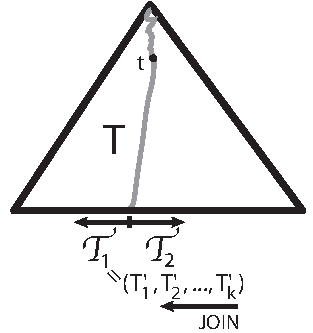
\includegraphics{pics/abtree-split}
\caption{Idea operace SPLIT}
\label{fig:abtree.split}
\end{figure}

P�epis operace SPLIT viz algoritmus \ref{alg:abtree.split}

\begin{algorithm}[!htb]
\caption{SPLIT pro $(a,b)$ stromy}
\label{alg:abtree.split}
\begin{algorithmic}
\ENSURE {Vytvo�� 
	$T_1$ reprezentuj�c� $\{ s \in S: s < x \}$ a
	$T_2$ reprezentuj�c� $\{ s \in S: s > x \}$}
\STATE Nech� $Z_1$ a $Z_2$ jsou pr�zdn� z�sobn�ky
\STATE $t := \text{ko�en } T$
\WHILE {$t$ nen� list}
	\STATE $i := 1$
	\WHILE {$H_t[i] < x \land i < \rho_t$}
		\STATE $i := i + 1$ 
	\ENDWHILE
	\STATE Vytvo� strom $T_1$, jeho� ko�en %$t_1$
	m� syny $S_t[1] \dots S_t[i-1]$
	\STATE Vytvo� strom $T_2$, jeho� ko�en %$t_2$
	m� syny $S_t[i+1] \dots S_t[\rho_t]$
	\IF {$T_1$ nen� jednoprvkov� strom}
		\STATE Push($Z_1, T_1$)
	\ENDIF
        \IF {$T_2$ nen� jednoprvkov� strom}
		\STATE Push($Z_2, T_2$)
	\ENDIF
	\STATE $t := S_t[i]$ 
\ENDWHILE
\IF {$t$ reprezentuje prvek r�zn� od $x$}
	\STATE Ud�lej z $t$ $(a,b)$ strom a vlo� ho
	do p��slu�n�ho z�sobn�ku.
\ENDIF
\STATE $T_1 := \text{STACKJOIN}(Z_1)$ \COMMENT {viz d�le}
\STATE $T_2 := \text{STACKJOIN}(Z_2)$
\end{algorithmic}
\end{algorithm}

\subsubsection{�asov� slo�itost operace SPLIT}

�as roz�ez�v�n� stromu je �m�rn� jeho hloubce. Celkov� �as operace
SPLIT ov�em z�vis� je�t� na slo�itosti operace STACKJOIN.

% ..........................................................................
\subsection{Algoritmus STACKJOIN($Z$) pro z�sobn�k $(a,b)$ strom�}
\label{abtrees.stackjoin}

Operace STACKJOIN provede JOIN v�ech (a,b)-strom� ulo�en�ch na z�sobn�ku.
V�sledkem je jedin� (a,b)-strom.

P�epis viz algoritmus \ref{alg:abtree.stackjoin}

\begin{algorithm}[!htb]
\caption{STACKJOIN pro $(a,b)$ stromy}
\label{alg:abtree.stackjoin}
\begin{algorithmic}
\STATE $T := \text{Pop}(Z)$
\WHILE {$Z \ne \emptyset$}
	\STATE $T' := \text{Pop}(Z)$
	\STATE $T := \text{JOIN}(T, T')$
\ENDWHILE
\end{algorithmic}
\end{algorithm}

\subsubsection{�asov� slo�itost operace STACKJOIN}

Nech� $Z$ obsahuje $(a,b)$ stromy $T_1 \dots T_k$, p�i�em� $T_1$ je
vrchol z�sobn�ku.
Plat�
\[
\forall i:\ \text{hloubka }T_i \leq \text{hloubka }T_{i+1}
\]
\begin{align*}
\text{�as STACKJOIN}
 & = \text{hloubka }T_2 - \text{hloubka }T_1 + 1 \\
 & + \text{hloubka }T_3 - \text{hloubka }T_2 + 1 \\
 & + \dots \\
 & + \text{hloubka }T_k - \text{hloubka }T_{k-1} + 1 \\
 & = \text{hloubka }T_k - \text{hloubka }T_1 + \text{po�et JOIN�} \\
 & = O(\text{hloubka }T) = O(\log |S|)
\end{align*}

Tedy i operace SPLIT vy�aduje �as $O(\log |S|)$.

% ..........................................................................
\subsection{Algoritmus FIND($T, k$) pro $(a,b)$ strom}

Nalezen� $k$-t�ho nejmen��ho prvku.

Roz����me reprezentaci stromu a ka�d�mu vnit�n�mu vrcholu $v$ p�id�me:
\begin{itemize}
\item $K_v[1\ .. \ \rho_v]$: $K_v[i]$ je po�et list�
v~podstromu $S_v[i]$ 
\end{itemize}

viz algoritmus \ref{alg:abtree.find}

\begin{algorithm}[!htb]
\caption{FIND pro $(a,b)$ stromy}
\label{alg:abtree.find}
\begin{algorithmic}
\STATE $t := \text{ko�en }T$
\WHILE {$t$ nen� list}
	\STATE $i := 1$
	\WHILE {$K_t[i] < k \land i < \rho_t$}
		\STATE $k := k - K_t[i]$ 
		\STATE $i := i + 1$ 
	\ENDWHILE
	\STATE $t := S_t[i]$ 
\ENDWHILE
\IF {$k > 1$}
	\STATE \textbf{return} nil \COMMENT {$k > |S|$}
\ELSE
	\STATE \textbf{return} $t$
\ENDIF
\end{algorithmic}
\end{algorithm}

�asov� slo�itost je op�t logaritmick�, p�i�em� d��ve uveden� operace
nejsou zpomaleny t�m, �e aktualizuj� pole (seznam) $K$.

% ..........................................................................
\section{A-sort}

Na prvn� pohled se zd�, �e pou�it� $(a,b)$ strom� ke t��d�n� nen�
v�hodn�. Pam�ov� n�roky budou oproti b�n�mu t��d�n� v poli asi
p�tkr�t v�t��. Aby se tedy t��d�n� $(a,b)$ stromem vyplatilo, muselo
by p�in�st zv��en� rychlosti. V t�to ��sti p�edvedeme, �e to skute�n�
je mo�n�, jestli�e vstupn� data jsou ji� ��ste�n� set��d�n�.

Pro ��ely A-sortu roz����me reprezentaci takto:
\begin{itemize}
\item Listy stromu jsou propojeny do seznamu
\item Je zn�ma cesta z nejmen��ho (nejlev�j��ho) listu do ko�ene
(ulo�en� nap�. v z�sobn�ku)
\end{itemize}

Pou�ijeme $(2,3)$-strom. Pro�, to si zd�vodn�me a� po odvozen� slo�itosti
A-sortu.

Nech� vstupn� posloupnost je $a_1, \dots, a_n$. Postupn� odzadu
vkl�d�me jej� prvky do stromu modifikovan�m INSERTem:

\begin{algorithmic}
\STATE $k := n$
\WHILE {$k > 1$}
	\STATE A-INSERT($a_k$)
	\STATE $k := k - 1$
\ENDWHILE
\end{algorithmic}

Na konci p�e�teme set��d�nou posloupnost pomoc� spojov�ho seznamu
list�.

\subsection{A-INSERT}

A-INSERT (viz algoritmus \ref{alg:abtree.a-insert}) pracuje
t�m�� stejn� jako p�vodn� INSERT - najde spr�vn� list a potom
p��padn� p�id� nov� prvek. K nalezen� spr�vn�ho listu ov�em vyu��v�
cestu z nejmen��ho listu. (viz obr. \ref{fig:abtree.a-insert})

\begin{figure} 
\centering\includegraphics{pics/a-insert}
\caption{Idea algoritmu A-INSERT}
\label{fig:abtree.a-insert}
\end{figure}

Zde uveden� verze A-INSERTu odstra�uje 
duplicitn� prvky, operaci lze pochopiteln� upravit tak, �e nech�v� 
duplicitn� prvky, kter� z�st�vaj� ve stejn�m po�ad�.

\begin{algorithm}[!htb]
\caption{A-INSERT($x$)}
\label{alg:abtree.a-insert}
\begin{algorithmic}
\STATE \COMMENT {Nalezen�}
\STATE $t := \text{nejmen�� list stromu } T$
\REPEAT
	\STATE $t := \text{otec } t$
\UNTIL {$t \text{ je ko�en} \lor x \leq H_t[1]$}
\STATE \COMMENT {nyn� jako v p�vodn�m INSERTu, pouze jsme jinak
inicializovali $t$}
\WHILE {$t$ nen� list}
	\STATE $i := 1$
	\WHILE {$H_t[i] < x \land i < \rho_t$}
		\STATE $i := i + 1$
	\ENDWHILE
	\STATE $t := S_t[i]$ 
\ENDWHILE
\STATE \COMMENT {P�id�n�}
\IF {$t$ nereprezentuje $x$}
	\STATE $o := \text{otec } t$
	\STATE vrcholu $o$ p�idej nov�ho syna $t'$ 
	reprezentuj�c�ho $x$
	\STATE za�a� $t'$ na spr�vn� m�sto mezi jeho bratry
	a uprav $\rho_o$, $S_o$ a $H_o$
	\STATE $t := o$
	\WHILE {$\rho_t > b$}
		\STATE \COMMENT {�t�pen� 
				--- m��eme prov�st d�ky podm�nce 4}
		\STATE rozd�l $t$ na $t_1$ a $t_2$ 
		\STATE \quad k $t_1$ dej prvn�ch 
			$\lfloor (b+1)/2 \rfloor$ syn� $t$
		\STATE \quad k $t_2$ dej zbyl�ch 
			$\lceil (b+1)/2 \rceil$ syn� $t$
		\STATE $o := \text{otec } t$
		\STATE uprav $\rho_o$, $S_o$ a $H_o$
		\STATE \COMMENT {p�i �t�pen� ko�ene je�t� mus�me
				vytvo�it nov� ko�en}
	\ENDWHILE
\ENDIF
\end{algorithmic}
\end{algorithm}

\subsection{Slo�itost A-sortu}

�as A-sortu
= $\sum$ �asu vyhled�n� + $\sum$ �asu p�id�n� + �as vytvo�en� v�stupn�
posloupnosti.
�as vytvo�en� v�stupn� posloupnosti = $O(n)$.

$\sum \text{�asu p�id�n�} 
= \text{po�et p�idan�ch vrchol�} \cdot \text{�as p�id�n� vrcholu}
+ \text{po�et �t�pen�} \cdot \text{�as �t�pen�}
= O(n) \cdot O(1)
+ \text{po�et �t�pen�} \cdot O(1).$ 
Proto�e se zde neprov�d� operace DELETE, lze ka�d�mu �t�pen� p�i�adit 
vnit�n� vrchol, kter� byl p�i tomto �t�pen� vytvo�en (�t�pen� rozd�l� 
vrchol $t$ na dva vrcholy $t_1$ a $t_2$, budeme p�edpokl�dat, �e 
vrchol $t_1$ je pokra�ov�n�m vrcholu $t$ a vrchol $t_2$ je vrchol 
vznikl� p�i �t�pen�). Tedy po�et �t�pen� je men�� ne� po�et vnit�n�ch 
vrchol� (p�i �t�pen� ko�ene vznik� nav�c je�t� nov� ko�en),  
tedy $\sum \text{�asu p�id�n�} = O(n).$

�as A-sortu tedy z�vis� hlavn� na celkov�m �ase vyhled�n� prvk�.
Ozna�me
\[
f_i = |\{ j > i:\ a_j < a_i \}|,
\]
tedy po�et prvk� posloupnosti, kter� v neset��d�n� posloupnosti
n�sleduj� $a_i$, ale v set��d�n� pat�� p�ed $a_i$. P�i vyhled�n� $a_i$
ve stromu vyjad�uje $f_i$ po�et list� nalevo od $a_i$. �as
vyhled�n� $a_i$ je tedy $O(\log f_i)$ a celkov� �as vyhled�n� je 
$O(\sum \log f_i)$.
\mnote{o�et�it $\log 0$}

Hodnota $F = \sum f_i$, zvan� 
\emph{po�et inverz�}, \mnote{nebo transpozic? standardn� term�n?}%
vyjad�uje uspo��danost vstupn�
posloupnosti. Pro spr�vn� uspo��danou posloupnost je $F = 0$, pro
obr�cen� uspo��danou posloupnost je $F = n (n-1) / 2$. To jsou tak�
mezn� hodnoty, jich� m��e $F$ nab�vat.

Z vlastnost� logaritmu a srovn�n�m geometrick�ho a aritmetick�ho
pr�m�ru dost�v�me
\[
\sum \log f_i = \log \prod f_i = n \log \sqrt[n]{\prod f_i}
\leq n \log (F/n).
\]

A-sort tedy vy�aduje �as $O(n \max(1, \log((F+1)/n)))$. V nejhor��m
p��pad� to je $O(n \log n)$ a Mehlhorn a Tsakalidis uk�zali, �e A-sort
je lep�� ne� Quicksort v p��pad�, �e $F \leq 0.02 n^{1.57}$.
Naproti tomu Insertsort, jednoduch� algoritmus, kter� postupn�
line�rn�m prohled�n�m zat�i�uje prvky pole do jeho ji� set��d�n�ho
po��te�n�ho �seku, vy�aduje �as $O(n + F)$, co� je v nejhor��m p��pad�
$O(n^2)$.

Zb�v� je�t� zd�vodnit, pro� pou��t $(2,3)$-stromy. V�me, �e $(2,3)$-stromy 
maj� nejmen�� prostorov� n�roky mezi $(a,b)$-stromy. Na druh� stran� v�ak 
$(2,3)$-stromy v obecn�m p��pad� vy�aduj� zbyte�n� mnoho vyva�ovac�ch 
operac�, a proto jsou v�razn� pomalej�� ne� nap�. $(2,4)$-stromy. Proto�e 
v�ak A-sort nepou��v� operaci DELETE, uk�zali jsme (viz po�et operac� 
�t�pen�), �e pro A-sort to nen� pravda. Zde $(2,3)$-stromy pat�� mezi 
nejrychleji pracuj�c� $(a,b)$-stromy.

% --------------------------------------------------------------------------
\section{Paraleln� p��stup do $(a,b)$ strom�}

P�i operac�ch INSERT a DELETE jsme nejprve sestupovali stromem dol� a�
k list�m, potom jsme se vraceli nahoru a �t�pili nebo spojovali
vrcholy. To znemo��uje dovolit paraleln� p��stup do stromu. Procesu,
kter� je ve f�zi vyhled�n�, by se mohlo st�t, �e mu jin� proces zm�n�
strom ``pod rukama''. St�vaj�c� operace INSERT a DELETE tedy po�aduj�
v�lu�n� p��stup ke stromu.
\par
Nyn� p�edvedeme paraleln� verzi t�chto operac�, kde se �t�pen� nebo
spojov�n� prov�d� ji� p�i sestupu. Potom ji� nen� nutn� se vracet a je
tedy mo�n� rovnou odemykat ��sti stromu, ke kter�m ji� dan� proces
nebude p�istupovat. Cenou za tento p��stup jsou zbyte�n�
�t�pen�/spojen�.
\mnote{ud�lat obr�zek ilustruj�c� zbyte�n� �/s}

Pot�ebujeme omezit $b$: podm�nku $b \geq 2a - 1$ zp��sn�me na
\begin{enumerate}
\item[4'.] $a \geq 2$ a $b \geq 2a$ 
\end{enumerate}

% ..........................................................................
\subsection{Paraleln� INSERT($x$) do $(a,b)$ stromu}

viz algoritmus \ref{alg:abtree.par.insert}

\begin{algorithm}[!htb]
\caption{paraleln� INSERT pro $(a,b)$ stromy}
\label{alg:abtree.par.insert}
\begin{algorithmic}
\STATE $o := \text{lock}(\text{nadko�en})$ \COMMENT {Nadko�en
je implementa�n� pom�cka. Slou�� k zamknut�
p��stupu k cel�mu stromu a uchov�v� $\max(S)$}
\STATE $t := \text{ko�en}$ 
\STATE \COMMENT {Invariant mezi pr�chody cyklem:
	$o$ je otec $t$, $o$ je jedin� vrchol zamknut� t�mto procesem.}
\WHILE {$t$ nen� list}
	\STATE $i := 1$
	\WHILE {$i < \rho_t \land H_t[i] < x$}
		\STATE $i := i + 1$
	\ENDWHILE
	\STATE $s := S_t[i]$ 
	\STATE \COMMENT {preventivn� roz�t�pen�:}
	\IF {$\rho(t) = b$}
		\STATE rozd�l $t$ na $t_1$ a $t_2$: \COMMENT {viz 4'}
		\STATE \quad k $t_1$ dej prvn�ch 
			$\lfloor (b+1)/2 \rfloor$ syn� $t$
		\STATE \quad k $t_2$ dej zbyl�ch 
			$\lceil (b+1)/2 \rceil$ syn� $t$
		\STATE \quad $t_1$ p�edch�z� $t_2$
		\STATE uprav $\rho_o$, $S_o$ a $H_o$
		\STATE \COMMENT {implic.: uprav $\rho_{t_1}$, \dots, $H_{t_2}$}
		\STATE \COMMENT {p�i �t�pen� ko�ene je�t� mus�me
				vytvo�it nov� ko�en}
		\STATE $n := t_j$, kde $s$ je syn $t_j$
	\ELSE
		\STATE $n := t$
	\ENDIF
	\STATE lock($n$) 
	\STATE unlock($o$) 
	\STATE $o := n$
	\STATE $t := s$
\ENDWHILE
\IF {$t$ nereprezentuje $x$}
	\STATE vrcholu $o$ p�idej nov�ho syna $t'$ 
	reprezentuj�c�ho $x$
	\STATE za�a� $t'$ na spr�vn� m�sto mezi jeho bratry
	a uprav $\rho_o$, $S_o$ a $H_o$
\ENDIF
\STATE unlock($o$)
\end{algorithmic}
\end{algorithm}

% ..........................................................................
\subsection{Paraleln� DELETE($x$) z $(a,b)$ stromu}

viz algoritmus \ref{alg:abtree.par.delete}

\begin{algorithm}[!htb]
\caption{paraleln� DELETE pro $(a,b)$ stromy}
\label{alg:abtree.par.delete}
\begin{algorithmic}
\STATE $o := \text{lock}(\text{nadko�en})$ \COMMENT {Nadko�en
je implementa�n� pom�cka. Slou�� k zamknut�
p��stupu k cel�mu stromu a uchov�v� $\max(S)$}
\STATE $t := \text{ko�en}$ 
\STATE $h := \textbf{nil}$ \COMMENT 
	{Jakmile $h \neq \textbf{nil}$, 
	$x \in H_h$ a $h$ bude zam�en� do konce procesu.}
\STATE \COMMENT {Invariant mezi pr�chody cyklem:
	$o$ je otec $t$, $o$ je krom� $h$ jedin� vrchol
	zamknut� t�mto procesem.}
\WHILE {$t$ nen� list}
	\STATE $i := 1$
	\WHILE {$i < \rho_t \land H_t[i] < x$}
		\STATE $i := i + 1$
	\ENDWHILE
	\IF {$H_t[i] = x$}
		\STATE $h := t$
	\ENDIF
	\STATE $s := S_t[i]$ 
	\STATE \COMMENT {preventivn� spojen�/p�esun:}
	\IF {$\rho(t) = a$}
		\STATE $v := \text{bezprost�edn� bratr } t$ %bratr[fi]=_v_eli
		\IF[sm�me spojit] {$\rho_v = a$}
			\STATE \COMMENT {Spojen�}
			\STATE slu� $v$ a $t$ do $t$ \COMMENT {viz 4'}
			\STATE uprav $\rho_o$, $S_o$ a $H_o$
			\STATE $t := o$
		\ELSE[$\rho_v > a$, spojen� by m�lo v�ce ne� $b$ syn�]
			\STATE \COMMENT {P�esun}
			\STATE p�esu� krajn�ho syna $v$ do $t$
			\STATE uprav $H_o$, $H_v$ a $H_t$
		\ENDIF
	\ENDIF
	\STATE lock($t$) 
	\IF {$o \neq h$}
		\STATE unlock($o$)
	\ENDIF
	\STATE $o := t$
	\STATE $t := s$
\ENDWHILE
\IF {$t$ reprezentuje $x$}
	\STATE odstra� $t$
	\STATE uprav $H_o$, $H_h$
	\STATE uprav $S_o$ a $\rho_o$
	\STATE unlock($h$)
\ENDIF
\STATE unlock($o$)
\end{algorithmic}
\end{algorithm}


% --------------------------------------------------------------------------
\section{Slo�itost posloupnosti operac� na $(a,b)$ stromu}

A-sort funguje jednak proto, �e v p�edt��d�n� posloupnosti rychle
najde m�sto, kam se m� vkl�dat, jednak proto, �e se p�i sam�ch
INSERTech ({\it a d�ky spr�vn�m $a$, $b$?}) prov�d� m�lo
vyva�ovac�ch krok�. V t�to sekci se pod�v�me na po�et vyva�ovac�ch
krok� pro posloupnost operac� INSERT a DELETE.

Nech� $b \geq 2a$.
\begin{theorem}
M�jme posloupnost $n$ operac� INSERT a DELETE aplikovanou na pr�zdn�
$(a,b)$ strom. Ozna�me $P$ po�et p�esun� p�i prov�d�n� posloupnosti,
$SP$ po�et spojen� a $ST$ po�et �t�pen�. D�le ozna�me $P_h$, $SP_h$ a
$ST_h$ po�et p�esun�. spojen� a �t�pen�, kter� nastanou ve v��ce $h$
(listy maj� v��ku 0).

Nech�
\begin{equation}
\begin{split}
% this is ``occult alignment'' :)
c = \min
 &\left(
   \phantom{b - \vphantom{x}}
        \min \left( 2a-1, \left\lceil \frac{b+1}{2}\right\rceil  \right) - a, 
  \right.\\
 &\left.
		\phantom{\left(
		\vphantom{\left. \frac xy\right.}
		\right.}
    b - \max \left( 2a-1, \left\lfloor\frac{b+1}{2}\right\rfloor \right)
   \phantom{\vphantom{x} - a}
  \right)
\end{split}
\end{equation}

Pak plat�
%\renewcommand{\labelenumi}{\alph{enumi}}
\begin{eqnarray}
P &\leq& n \\
\label{ab-v-stsp}
(2c-1)ST + cSP &\leq& n + c + \frac c{a+c-1} (n-2) \\
\label{ab-v-sthsph}
P_h + SP_h + ST_h &\leq& \frac{2 n^{c+2}}{(c+1)^h} 
\end{eqnarray}
\end{theorem}

Plat� $c \geq 1$ (p�i $b = 2a$ dokonce $c = 1$). Z toho
\begin{equation}
ST + SP \leq \frac nc + 1 + \frac{n-2}a,
\end{equation}
tedy line�rn� vzhledem k $n$.

Pro paraleln� verze INSERT a DELETE plat� obdobn� v�ta, kdy� 
$b \geq 2a + 2$.

Pro d�kaz pou�ijeme \emph{bankovn� paradigma}: datovou strukturu
ohodnot�me podle toho, jak je ``uklizen�''. Operace, kter� datovou
strukturu ``uklid�'', zv�t�� jej� ``z�statek na ��t�''. Ty, kter� ji
``naru��'', z�statek zmen��. Potom najdeme vztah mezi z�statkem a
spot�ebovan�m �asem.
{\it Tohle pokulh�v�. Myslel jsem si, �e z�statek je n�co jako �as v
konzerv�, kter� si pomal� operace berou od rychl�ch \dots, ale  v
tomhle p��pad� to asi funguje jinak.}
\mnote{vyjasnit}
\mnote{pou�iju $z$ jako z�statek m�sto $b$ jako balance, proto�e
souvislost s vyva�ov�n�m stromu je zde sp�� matouc�}

$(a,b)$ stromy jsou uklizen�, kdy� maj� vrcholy po�et syn� n�kde
uprost�ed mezi $a$ a $b$. Tehdy nenastane v brzk� dob� vyva�ovac�
operace. V tomto smyslu definujme:
\begin{align}
z(v) &=
	\min ( \rho_v - a, b - \rho_v, c ) 
	&&\text{$v$ je vnit�n� vrchol r�zn� od ko�ene}\\
z(\text{ko�en}) &=
        \min ( \rho_v - 2, b - \rho_v, c ) 
\end{align}

Pro strom $T$ definujme 
\[
z(T) = \sum_{v \in T} z(v)
\]
\[
z_h(T) = \sum_{\substack{v \in T\\v \text{ m� v��ku } h}} z(v)
\]
Plat�
\[
z(T) = \sum_h z_h(t)
\]

Podobn� jako u �erveno�ern�ch strom� definujme parci�ln� $(a,b)$-strom:
\begin{defn}
$(T,v)$ je \emph{parci�ln� $(a,b)$-strom,} kdy� $v$ je vnit�n� vrchol $T$
r�zn� od ko�ene a
krom� $v$ jsou spln�ny podm�nky pro $(a,b)$-strom a
$a-1 \leq \rho_v \leq b+1$.
\end{defn}

Z definice z�statku vypl�vaj� tyto vlastnosti:
\begin{align}
\label{ab-1}
  \rho_v = a-1 \text{ nebo }b+1 &\implies z(v) = -1\\
\label{ab-0}
  \rho_v = a \text{ nebo } b    &\implies z(v) = 0\\
\label{ab-spojeni}
  \rho_v = 2a-1                 &\implies z(v) = c\\
\label{ab-stepeni}
  \rho_u = \left\lfloor\frac{b+1}{2}\right\rfloor \land
  \rho_v = \left\lceil \frac{b+1}{2}\right\rceil
                                &\implies z(u)+z(v) \geq 2c - 1\\
\label{ab-presun}
  |\rho_u - \rho_v| \leq 1      &\implies z(u) \geq z(v) - 1
\end{align}

\subsection{P�id�n�/ubr�n� listu}

M�jme $(a,b)$-strom $T$ a p�id�me nebo ubereme list, jeho� otec je $v$.
Pak vznikne parci�ln� $(a,b)$-strom $(T',v)$ a plat�:
\begin{align}
  z_1(T')        & \geq z_1(T) - 1\\
  z_h(T')        & = z_h(T) \quad h>1\\
  z(T')          & \geq z(T) - 1
\end{align}

\subsection{�t�pen�}

M�jme parci�ln� $(a,b)$-strom $(T,v)$, kde $v$ je ve v��ce $h$.
Nech� $T'$ vznikl \emph{�t�pen�m $v$}. 
Pak $(T',\text{otec }v$ je parci�ln� $(a,b)$-strom a plat�:
\begin{align}
  z_h(T')       & \geq 2c + z_h(T)
	\qquad\text{z \ref{ab-1} a \ref{ab-stepeni}}\\
  z_{h+1}(T')   & \geq z_{h+1}(T) - 1\\
  z_i(T')       & = z_i(T) \quad i \neq h, h+1\\
  z(T')         & \geq z(T) + 2c - 1
\end{align}

\subsection{Spojen�}

M�jme parci�ln� $(a,b)$-strom $(T,v)$, kde $\rho_v = a-1$ a 
$v$ je ve v��ce $h$, $y$ je bezprost�edn� bratr $v$.
Nech� $\rho_y = a$ a $T'$ vznikl \emph{spojen�m $v$ a $y$}. 
Pak $(T',\text{otec }v$ je parci�ln� $(a,b)$-strom a plat�:
\begin{align}
  z_h(T')       & \geq c + 1 + z_h(T)
	\qquad\text{z \ref{ab-1}, \ref{ab-0} a \ref{ab-spojeni}}\\
  z_{h+1}(T')   & \geq z_{h+1}(T) - 1\\
  z_i(T')       & = z_i(T) \quad i \neq h, h+1\\
  z(T')         & \geq z(T) + c
\end{align}

\subsection{P�esun}

M�jme parci�ln� $(a,b)$-strom $(T,v)$, kde $\rho_v = a-1$ a 
$v$ je ve v��ce $h$, $y$ je bezprost�edn� bratr $v$.
Nech� $\rho_y > a$ a $T'$ vznikl \emph{p�esunem syna od $y$ k $v$}. 
Pak $T'$ je $(a,b)$-strom a plat�:
\begin{align}
  z_h(T')       & \geq z_h(T)
	\qquad\text{z \ref{ab-1}, \ref{ab-0} a \ref{ab-presun}}\\
  z_i(T')       & = z_i(T) \quad i \neq h\\
  z(T')         & \geq z(T)
\end{align}

Nech� po skon�en� posloupnosti operac� m�me $(a,b)$-strom $T_k$.
Se�teme p�edchoz� v�sledky:
\begin{equation}
\label{eq:ab-secti}
  z(T_k) \geq (2c - 1)ST + c SP - n  
\end{equation}

\begin{align}
  z_1(T_k)      & \geq 2c ST_1 + (c+1) SP_1 - n\\
  z_h(T_k)      & \geq 2c ST_h + (c+1) SP_h - ST_{h-1} - SP_{h-1} \quad h>1
\end{align}
Vad� n�m, �e jsou ve v�razu i spojen� a �t�pen� z jin� hladiny.

$c \geq 1 \implies 2c \geq c+1$.
\[
  z_h(T_k) \geq (c+1) (ST_h + SP_h) - ST_{h-1} - SP_{h-1}
\]
\begin{align}
  ST_h + SP_h 
&  \leq \frac{z_h(T_k)}{c+1} + \frac{ST_{h-1} + SP_{h-1}}{c+1}
  \leq \frac{z_h(T_k)}{c+1} + 
         \frac{z_{h-1}(T_k)}{(c+1)^2} + 
         \frac{ST_{h-2} + SP_{h-2}}{(c+1)^2}\\
&  \leq \left( \sum_{i=0}^{h-1} \frac{z_{h-i}(T_k)}{(c+1)^{i+1}} \right) + 
         \frac{ST_0 + SP_0}{(c+1)^h}
                \qquad\text{$j=h-i$, roz����me $(c+1)^{h-i}$}\\
\label{ab-sthsph}
&  = \left( \sum_{j=1}^h \frac{z_j(T_k)(c+1)^j}{(c+1)^{h+1}} \right) + 
         \frac{n}{(c+1)^h}
\end{align}

Nech� $T$ je $(a,b)$-strom s $m$ listy. Chceme shora odhadnout $z(T)$.
\begin{equation}
  m_j = \text{po�et vnit�n�ch vrchol� r�zn�ch od ko�ene}
  \begin{cases}
    \text{s pr�v� $a+j$ syny}   & \text{kdy�}\ j \in\intrange{0}{c-1}\\
    \text{s alespo� $a+j$ syny} & \text{kdy�}\ j = c
  \end{cases}
\end{equation}

Kdy� $v$ je vnit�n� vrchol r�zn� od ko�ene s pr�v� $a+j$ syny,
$j \in\intrange{0}{c-1}$,
pak $z(v) \leq j$.

Kdy� $v$ je vnit�n� vrchol r�zn� od ko�ene s alespo� $a+c$ syny,
pak $z(v) \leq c$.

Tedy
\begin{equation}
  \label{eq:ab-mj}
  z(T) \leq c + \sum_{j=0}^c j m_j = *
\end{equation}

Spo��t�me hrany v $T$: nalevo jsou hrany vych�zej�c� z ko�ene a
vnit�n�ch vrchol�, napravo jsou hrany p�ich�zej�c� do vnit�n�ch
vrchol� a list�.
\begin{equation}
2 + \sum_{j=0}^c (a+j) m_j \leq
\text{po�et hran}
= \left( \sum_{j=0}^c m_j \right) + m
\end{equation}
Tedy $m-2 \geq \sum_{j=0}^c (a+j-1) m_j$.

\begin{equation}
  *
  =    c + \sum_{j=0}^c \frac{j}{a+j-1}(a+j-1) m_j 
  \leq c + \sum_{j=0}^c \frac{c}{a+c-1}(a+j-1) m_j 
  \leq c + \frac{c}{a+c-1} (m-2)
\end{equation}

Spojen�m tohoto v�sledku s \ref{eq:ab-secti} dostaneme \ref{ab-v-stsp}.

K d�kazu \ref{ab-v-sthsph} vyu�ijeme \ref{ab-sthsph}.
\begin{equation}
  m_{h,j} = \text{po�et vnit�n�ch vrchol� ve v��ce $h$}
  \begin{cases}
    \text{s pr�v� $a+j$ syny}   & \text{kdy�}\ j \in\intrange{0}{c-1}\\
    \text{s alespo� $a+j$ syny} & \text{kdy�}\ j = c
  \end{cases}
\end{equation}

\begin{equation}
  z_h(T) \leq \sum_{j=0}^c j m_{h,j}
\end{equation}
\begin{equation}
  \sum_{j=0}^c m_{h,j}
   = \text{po�et vrchol� ve v��ce $h$} 
  \geq \sum_{j=0}^c (a+j) m_{h+1,j}
\end{equation}
\begin{equation}
\label{ab-x}
  \sum_{j=0}^c j m_{h,j}
  \leq \sum_{j=0}^c m_{i-1,j} - a \sum_{j=0}^c m_{i,j} 
\end{equation}
\begin{align}
   \sum_{i=1}^h z_i(T_k)(c+1)^i
 & \leq \sum_{i=1}^h (c+1)^i \left( \sum_{j=0}^c j m_{i,j} \right) \\
\intertext{ozna�me $s_i = \sum_{j=0}^c m_{i,j}$}
 & \stackrel{\text{\ref{ab-x}}}{\leq} 
        \sum_{i=1}^h (c+1)^i \left( s_{i-1} - a s_i \right) \\
 & = (c+1)s_0 - (c+1)^h a s_h + 
        \sum_{i=2}^h (c+1)^i \left( s_{i-1} - \frac{a}{c+1} s_{i-1} \right) \\
 & \leq (c+1) m \qquad\text{proto�e $\frac{a}{c+1} \geq 1$ a $s_0 = m$}
\end{align}

\[
ST_h + SP+h \leq \frac{m}{(c+1)^h} + \frac{n}{(c+1)^h} \leq \frac{2n}{(c+1)^h}
\]
\[
P_h \leq SP_{h-1} - SP_h \leq SP_{h-1} + ST_{h-1} \leq \frac{2n}{(c+1)^{h-1}}
\]
T�m dost�v�me \ref{ab-v-sthsph}:
\[
ST_h + SP_h + P_h \leq \frac{2 n (c+2)}{(c+1)^h}
\]


% --------------------------------------------------------------------------
\section{Propojen� $(a,b)$ stromy s prstem}

Variantou $(a,b)$ strom� jsou $(a,b)$ stromy, kter� maj� propojen�
jednotliv� hladiny a d�le obsahuj� ukazatel na jeden z list�.
T�mto strom�m se tak� n�kdy ��k� jenom stromy s prstem (p�edpokl�d� se, �e
jsou propojen�) nebo hladinov� propojen�. V anglick� literatu�e se
vyskytuj� pod pojmem \emph{finger trees}.
\par
Struktura vnit�n�ho vrcholu $v$ obsahuje n�sleduj�c� polo�ky: 
\begin{itemize}
\item $\rho(v) =$ po�et syn� $v$ 
\item $Syn[1..\rho(v)]$ je pole ukazatel� na syny vrcholu $v$
\item $Hod[1..\rho(v)]$ je pole hodnot, plat� 
\item $Hod(i-1) <$ prvky reprezentovan� v podstromu $i$-t�ho syna $\leq Hod(i)$ 
\item $otec(v)$ = ukazatel na otce vrcholu $v$
\end{itemize}

\begin{tabular}{l}
P�edch�dce$(v)$ \\
N�sledn�k$(v)$
\end{tabular}
$\Bigl\}$
\begin{tabular}{l}
ukazatele na bezprost�. p�edch�dce (n�sledn�ka) v na hladin� vrcholu $v$ \\
(v lexikogr. uspo��d�n�)
\end{tabular}
\par

$h$ - hodnota, kter� le�� mezi nejv�t��m prvkem podstromu v a nejmen��m
prvek podstromu n�sledn�ka.

P��klad (a,b)-stromu s prstem je vid�t na obr. \ref{fig.abtree.finger}

\begin{figure}[!htb]
\centering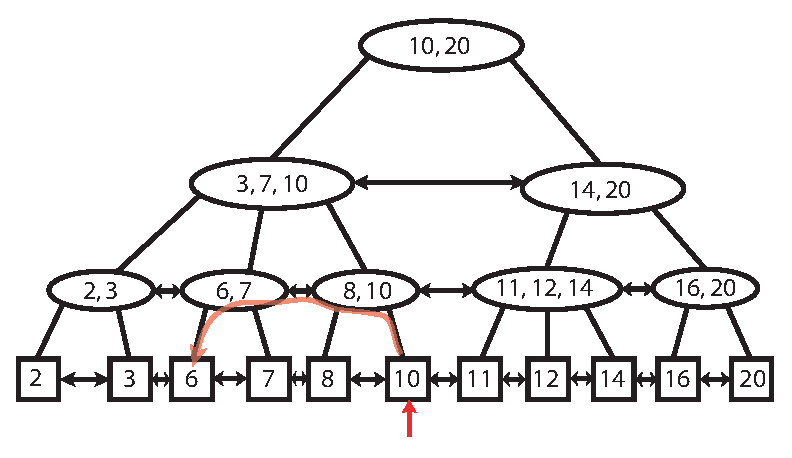
\includegraphics{pics/abtree-finger}
\caption{(a,b)-strom s prstem p�i proveden� operace MEMBER(6)} 
\label{fig.abtree.finger}
\end{figure} 

\subsection{Algoritmus MEMBER}

Viz algoritmus \ref{alg:abtreesfing.member}

\mnote{XXX alg. MEMBER je velmi podivny, prepracovat}

\begin{algorithm}[!htb]
\caption{MEMBER (a,b) stromy s prstem}
\label{alg:abtreesfing.member}
\begin{algorithmic}
\STATE MEMBER(x)
\STATE 1) Nech� $y$ je hodnota, na kterou ukazuje Prst.
  \IF {$x < y$} 
    \STATE pokra�uju 2)
  \ELSE
    \STATE 3)
  \ENDIF
\STATE 2) $v \leftarrow otec(y)$
  \STATE dokud $x < h$(P�edch�dce(P�edch�dce($v$))
   \STATE jdu na otce(P�edch�dce($v$))
  \STATE v opa�n�m p��pad�
    \STATE kdy� $x \leq$ h(P�edch�dce($v$)) pak
    \STATE $v$ $\leftarrow$ P�edch�dce($v$)
    \STATE a pokra�uji norm�ln�m vyhled�v�n�m
\STATE 3) symetrick� ke 2)
\end{algorithmic}
\end{algorithm}

\subsection{Algoritmus FINGER}

FINGER($x$) \\
nastav� hodnotu na list, kter� reprezentuje prvek nejbli��� k x.

Pou�it�: \\
kdy� lze operace p�irozen�m zp�sobem rozd�lit do segment� a operace v ?
segmentu maj� operace bl�zko sebe
\par

\begin{itemize}
\item vyhled�n� $x$ vy�aduje �as $O(1 + \log(l))$
\item nastav�m prst na n�jakou vhodnou hodnotu
\end{itemize}

\begin{theorem}
Nech� $T$ je propojovan� (a,b) strom s prstem a nech� $P$ je posloupnost
p��kaz� MEMBER, INSERT, DELETE, FINGER, kterou provedeme na $T$.
Pak $P$ vy�aduje �as $O(log(n) + \text{�as na vyhled�n�})$
kde $n$ je velikost mno�iny reprezentovan� stromem $T$. ($b \geq 2a$)
\end{theorem}

\subsection{Amortizovan� slo�itost}

Vezmeme posloupnost $n$ operac�, spo��t�me maxim�ln� �as, kter� vy�aduj� a
ten vyd�l�me $n$. 
Limita takto z�skan�ch ��sel pro $n \rightarrow \infty$ je amortizovan�
slo�itost.

\subsubsection{Bankovn� paradigma}

Pou�ijeme n�sleduj�c� zna�en� pro p�echodu mezi stavy (situacemi):
$D \stackrel{o}{\rightarrow} D'$

\begin{itemize}
\item $D$ - vstupn� situace 
\item $o$ - operace 
\item $D'$ - v�stupn� operace 
\end{itemize}

Amortizovan� slo�itost operace $o$ je �as$(O) + bal(D') - bal(D)$,
kde $bal()$ je ohodnocen� konfigurace.

$D_0 \stackrel{O_1}{\rightarrow} D_1 \stackrel{O_2}{\rightarrow} D_2 \rightarrow \ldots \rightarrow D_n$

$$\sum_{i=1}^{n} \text{�as}(O_i) + bal(D_n) - bal(D_0) = \sum a(O_i) \leq
\sum i(O_i)$$

Obvykle plat�, �e $bal \geq 0$ nebo $bal \leq 0$. \\
Kdy� $bal \geq 0$, pak: \\
  $$\sum \text{�as}(O_i) \leq \sum a(O_i) + bal(D_0) \leq \sum i(O_i) + bal(D_0)$$
Kdy� $bal \leq 0$, pak \\
  $$\sum \text{�as}(O_i) \leq \sum a(O_i) - bal(D_n) \leq \sum i(O_i) - bal(D_0)$$

Za��n�me na pr�zdn�m (a,b) strom� $\rightarrow bal = 0$.

XXX nechybi tady neco ?



% ==========================================================================
% Sou��st skript na Datov� struktury. Viz main.tex
% p�epsal Vladim�r Kotal, 2003


% nasleduje prednaska z 19.3.2003, p�epsal Vladim�r Kotal

\markright{$ $Id$ $}

\chapter{Samoopravuj�c� se struktury}

Upravuj�c� algoritmy pracuj� na seznamech, mohou p�em�stit prvek, 
kter� je argumentem operace. (pokud z�st�v� v seznamu) 
�as na vyhled�n� - to je pozice hledan�ho prvku. Pokud nen� v seznamu, je
to d�lka seznamu + 1.
\par

Pokud byl prvek na i-t�m m�st� a p�esune se na j-t�, tak je-li\\
  j $<$ i , provedou i-j voln�ch v�m�n\\
  j $>$ i , provedou j-i placen�ch v�m�n
\par

Voln� v�m�ny se nezapo��t�vaj� do slo�itosti.
Pokud x nen� v seznamu p�i operaci INSERT(x), tak p�edpokl�dejme, �e je na
1. pozici po ukon�en� seznamu.


% --------------------------------------------------------------------------
\section{Amortizovan� slo�itost}

XXX

% --------------------------------------------------------------------------
\section{Seznamy}

XXX

\subsection{Algoritmus MEMBER}

XXX

\subsection{Algoritmus INSERT}

XXX

\subsection{Algoritmus DELETE}

XXX

\subsection{Algoritmus MFR (Move Front Rule)}
% p�edn�ka z 18.3.2003
P�i operaci MEMBER(x) je x v seznamu nebo p�i operaci INSERT(x)
bude x po skon�en� operace na 1. m�st� seznamu.

\begin{theorem}
M�jme posloupnost P operac� MEMBER, INSERT a DELETE a m�jme dva
prost� seznamy S1, S2 mno�iny S. \\
Pak pro ka�d� upravuj�c� algoritmus A plat�:\\
Kdy� MFR provede P na seznam S1 a A provede P a seznam S2, tak plat�:\\
% XXX udelat seznam
\begin{itemize}
\item{a)} �as MFR $\leq$ �as na vyhled�n� A + po�et placen�ch v�m�n A - po�et voln�ch
v�m�n A - $|P|$ 
  kdy� S1 = S2 \\
\item{b)} �as MFR $\leq$ �as na vyhled�n� A + po�et placen�ch v�m�n A - po�et voln�ch
v�m�n A - $|P|$ + $\binom{|S|}{2}$ 
  kdy� S1 $\neq$ S2
\end{itemize}
\end{theorem}

\begin{defn}
Nech� S1, S2 jsou dva prost� seznamy mno�iny S, pak bal(S1,S2) je
po�et neuspo��dan�ch dvojic {x,y}, x $\neq$ y, x,y $\in$ S takov�ch �e x
je p�ed y v S1 a y je p�ed x v S2.
\end{defn}

\begin{pozn}
Plat� \\
bal(S1,S2) = 0 $\Leftrightarrow$ S1 = S2 (prvky jsou ve stejn�m
po�ad� $\Leftrightarrow$ seznamy jsou stejn�)\\
bal(S1,S2) $\leq$ $\binom{|S|}{2}$ (v�echny dvojice jsou p�eh�zen�)
\end{pozn}

\begin{proof}[D�kaz v�ty XXX] 
P�es amortizovanou slo�itost A. \\
P�edpokl�dejme, �e A i MFR maj� prov�st operaci O.\\
A ... prov�d� na seznam $S_A$, v�sledek bude $S_A'$ \\
MFR .. prov�d� O na seznam $S_{MFR}$, v�sledek bude $S_{MFR}'$\\
amortizovan� slo�itost operace O bude
  �as MFER pro operaci O + bal($S_A'$, $S_{MFR}'$) - bal($S_A$,
$S_{MFR}$)\\
balance je def. vzhledem k algoritmu A.
\par

Uk�eme, �e amortizovan� slo�itost O pro MFR $\leq$ 2*�as na vyhled�n� A +
po�et placen�ch v�m�n A - po�et voln�ch v�m�n A - 1
\par

$$
{\rm S_A}\stackrel{vyhled�n�}{\rightarrow} S_A''
\stackrel{v�m�ny}{\rightarrow} S_A'
% XXX cestina
$$
$$
{\rm S_{MFR}} \rightarrow S_{MFR}' \rightarrow S_{MFR}'
% XXX carkovana sipka
$$
\par

kde po operaci \\

\begin{tabular}{|l|l|}
\hline
DELETE(x) & $S_A''$ = $S_A'$\\
MEMBER(x) & $S_A''$ = $S_A$\\
INSERT(x) & x je v seznamu , $S_A''$ = $S_A$\\
  	  & x nen� v seznamu, $S_A''$ vznikne z $S_A'$ p�id�n�m x za
posledn� prvek seznamu\\
\hline
\end{tabular}

% \(
% \begin{cases}
%  x\ je\ v\ seznamu , S_A'' = S_A\\
%  x\ nen�\ v\ seznamu, S_A''\ vznikne\ z\ S_A'\ p�id�n�m\ x za posledn� prvek seznamu
% \end{cases}
% \)


Podstatn� je, �e seznamy jsou nad stejnou mno�inou
\par

Amort. slo�itost prvn� ��sti $\leq$ 2*�as na vyhled�n� pro A - 1\\
Amort. slo�itost druh� ��sti = po�et placen�ch v�m�n A - po�et voln�ch
v�m�n A
\par

% XXX jak donutit itemize aby cislovalo pomoci i, ii, iii, ... ?
\begin{itemize}
\item{(i)}
P�edpokl�dejme, �e x nen� v seznamu a d�lka seznam� je n.
�as MFR je n+1 , �as na vyhled�n� pro algoritmus je n+1
operace MEMBER(x) a DELETE(x) $S_A''$ = $S_{MFR}'$
a tady amort. slo�. MFR = �as operace = n++ $\leq$ 2(n+1) - 1\\
n+1 je �as na vyhled�n� pro A - 1\\
$S_A''$ vznikne z $S_A$ p�id�n�m x za posl. prvek $S_A$\\
$S_{MFR}'$ vznikne z $S_{MFR}$ p�id�n�m x na za�. seznamu
tedy bal($S_A''$, $S_{MFR}'$) - bal($S_A$, $S_{MFR}$) = n\\
Amort. slo�. operace MFR = n+1 + n=2n + 1=2(n+1) - 1 = 2*�as na vyhled�n�
A - 1

\item{(ii)} x je v seznamu. P�edpokl�dejme, �e x je na i-t�m m�st� v seznamu $S_A$
					na j-t�m m�st� v seznamu $S_{MFR}$
�as operace pro MFR je j, �as na vyhled�n� pro A je i.
Ozna�me k po�et y v seznamu takov�ch, �e y je v $S_A$ za x, v $S_{MFR}$ p�ed
x.
\par
Pak i+k $\geq$ j (i+k $\geq$ i-k+j)
amort. slo�. pro MFR = j + bal($S_A''$, $S_{MFR}'$) - bal($S_A$, $S_{MFR}$)
\par

DELETE(x)\\
bal($S_A''$, $S_{MFR}'$) - bal($S_A$, $S_{MFR}$) $\leq$ -k
amort. slo�. $\leq$ j - k $\leq$ 2i - 1 = 2*�as na vyhled�n� A - 1
\par

MEMBER(x), INSERT(x) \\
bal($S_A''$, $S_{MFR}'$) - bal($S_A$, $S_{MFR}$) $\leq$ -k + i-1
(n�jak� dvojice mohly p�ib�t)
amort. slo�. operace MFR $\leq$ j-k+i-1 $\leq$ i+i-1 = 2i - 1 = 2*�as na
vyhled�n� A-1
\par
\end{itemize}

\subsubsection{Amort. slo�itost}
1. f�ze operace $\leq$ 2*�as na vyhled�n� A-1
2. f�ze operace = po�et placen�ch v�m�n A - po�et voln�ch v�m�n A
P�i placen� v�m�n� si v seznamu $S_A''$ vym�n� x m�sto z za x, tedy
dvojice {x,z} p�ibude p�i po��t�n� bal($S_A'$, $S_{MFR}'$) - bal($S_A''$,
$S_{MFR}'$) (v $S_{MFR}$ je x prvn�)
P�i voln� v�m�n� se v seznamu $S_A''$ vym�n� x m�sto s prvkem u p�ed x,
tedy dvojice {x,u} se vynech� p�i po��t�n� bal.
Amort. slo�. MFR $\leq$ 2*�as na vyhled�n� A + po�et placen�ch v�m�n A -
po�et voln�ch v�m�n A - 1
\par

Tedy plat�: \\
�as posloupnosti P pro MFR $\leq$ odhad amort. slo�itosti + bal($S_1$,
$S_2$) = 2*�as na vyhled�n� v P algoritmem A + po�et placen�ch v�m�n A p�i
P - po�et voln�ch v�m�n A p�i P - $|P|$ + bal($S_1$, $S_2$)

\mnote{|P| ... za ka�dou operaci je -1}
kdy� $S_1$ = $S_2$ pak bal($S_1$, $S_2$)=0 a plat� a)
     $S_1$ $\neq$ $S_2$ pak bal($S_1$, $S_2$) $\leq$ $\binom{|S|}{2}$ a
plat� b)
\end{proof}

\begin{pozn}
S t�mto jsme se setkali p�i EISCH \\
       je to d�vod, pro� je EISCH lep�� ne� LISCH
			    VICH lep�� ne� LICH
\end{pozn}

\subsection{Algoritmus TR (Transposition Rule)}
Kdy� je x p�i operaci MEMBER(x) a INSERT(x) na i-t�m m�st�, tak ho d� na
(i-1)-n� m�sto, p�i INSERT(x), kdy x nen� v seznamu, d� x na p�edposl. m�sto.
\par

\begin{pozn}
Lze naj�t posloupnost p��kaz� P lib. d�lky, �e MFR vy�aduje �as $(|P|)$ a
TR vy�aduje �as $(|P|^2)$. Na druhou stranu o�ek�van� �as TR $\leq$
o�ek�van� �as MFR.
\end{pozn}


Chceme spo��tat o�ek�van� �as pro posloupnosti P aplikovan� na seznam S,
kde P obsahuje jen operace MEMBER(x) pro x $\in$ S. 
\par
P�edppokl�dejme, �e S={1,2, ... , n} a $\beta_1$ = pravd�podobnost operace
MEMBER(x) pro x $\in$ S.
S = \{1,2,3\} ... stavy Markovova �et�zce jsou v�echny permutace S
pravd�podobnost p�echodu je pst. operace p�ev�d�j�c� jeden stav do druh�ho
\par

\mnote{chybi obr.}
%\begin{figure}[!htb]
%\centering\includegraphics{pics/tr}
%\caption{P�echody mezi stavy}
%\label{tr-prechody}
%\end{figure}


Tyto Markovovy �et�zce jsou nerozlo�iteln� a aperiodick� a to znamen�, �e
existuj� asymptot. pravd�podobnosti, tj. pro seznam $\Pi$ je d�na
pravd�podobnost ${\kappa}_{\Pi}$, �e po proveden� n�hodn� posloupnosti P s
dan�m rozlo�en�m operac� skon��me u seznamu $\Pi$.
\par

Pak o�ek�van� �as je $\sum_{\Pi}{\kappa}_{\Pi}\sum_{i}{\beta}_i\Pi(i)$, 
$\Pi(i)$ je pozice i v seznamu $\Pi$.\\
$p_1 = \sum_{\Pi}{\kappa}_{\Pi}\Pi(i)$ ... o�ek�van� pozice prvku i
$\delta(j,i)$ = asmyptot. pst., �e prvek j je p�ed i, pak plat�\\
$$
\delta(j,i) = \sum\{\kappa_\Pi , \Pi\ seznam, \Pi(j) < \Pi(i)\}
$$

pak 
\begin{multline}\bigparens
\label{XXX-uprava}
p_i
= \sum_{\Pi}\kappa_\Pi\Pi(i)
= \sum_{\Pi}\kappa_\Pi(1 + |{j, \Pi(j) < \Pi(i)|}\\
= 1 + \sum{j,\Pi}\{kappa_\Pi, \Pi(j) < \Pi(i)\} = 1 + \sum_{j}\delta(j,i) (1)
\end{multline}

Zkus�me $\delta(j,i)$ spo��tat jin�m zp�sobem:\\
Idea: jak se m��e st�t, �e ve v�sledn�m seznamu je j p�ed i ?
V posloupnosti P existovala operace MEMBER(x) a po n� se u� nevyskytovala
operace MEMBER(i) ani MEMBER(j).
\par

Jak� je pravd�podobnost tohoto jevu ?
\begin{multline}
\beta_j\sum_{k=0}^{\infty}[1 - (\beta_i - \beta_j)]^k 
= \beta_j \frac{1}{1-(1-(\beta_i+\beta_j)} 
= \frac{\beta_j}{\beta_j+\beta_i} \stackrel{(1)}{=} 
1 + \sum_{\substack{j,i\\j \ne i}} \frac{\beta_j}{\beta_j+\beta_i}
\end{multline}

o�ek�van� �as operace je 
$$
\sum_{i} \beta_i p_i 
= \sum_{\substack{j,i\\j \ne i}} \frac{\beta_i\beta_j}{\beta_i+\beta_j}
$$

P�edpokl�dejme, �e $\beta_1 \geq \beta_2 \geq ... \geq \beta_n$ \\
pak nejrychlej�� algoritmus na seznam $x_1 - x_2 - ... - x_n$ je klasick�
algoritmus bez p�em�s�ov�n� prvk�. O�ek�van� �as tohoto algoritmu je 

\begin{multline}
\sum_{i=1}^{n}i\beta_i = \\
1 + \sum_{i,j=1} 2\frac{\beta_j\beta_i}{\beta_i+\beta_j} \leq 1 + 
  \sum_{\substack{i,j\\j<i}} 2\beta_i = 1 + \sum_{i=1}^{n} 2*(i-1)\beta_i =
\frac{\beta_j}{\beta_j+\beta_i} \leq 1 = \\
1 + 2\cdot\sum_{i}i\beta_i - 2\sum_{i}\beta_i = 
2\sum_{i=1}^{n}i\beta_i - 1
\end{multline}

% --------------------------------------------------------------------------
\section{Splay stromy}
% thanks to Jana Skotakova za zapisky, p�epsal Vladim�r Kotal

patov� struktura - bin�rn� vyhled�vac� stromy s ohodnocen�mi prvky


\subsection{Operace SPLAY}
Z�kladn� operac� je pr pr�ci s t�mito stromy je SPLAY(x), kter� zjist�,
zda x je reprezentov�n v dan� mno�in�. Pokud x le�� v mno�in�, algoritmus
ho p�em�st� do ko�ene.
\par
Kdy� x nele�� v mno�in�, pak algoritmus p�em�st� do ko�ene bu� nejmen��
prvek v�t�� ne� x nebo nejv�t�� prvek men�� ne� x (kter� le�� v reprez.
mno�in�)

\subsection{Podporovan� operace}
MEMBER, INSERT, DELETE, JOIN2($T_1$,$T_2$), JOIN3(x, $T_1$, $T_2$) 
(nebo asi taky JOIN3($T_1$, x, $T_2$)), SPLIT(x), 
CHANGEWEIGHT(x, $\triangle$).

JOIN2($T_1$,$T_2$)\\
p�edpokl�d�, �e $\forall$ prvky reprezentovan� $T_1 < \forall$ prvky
reprezentovan� $T_2$\\
v�sledn� strom reprezentuje $T_1 \cup T_2$.

JOIN3($T_1$, x, $T_2$)
p�edpokl�d�, �e $\forall$ prvky reprezentovan� $T_1 < x < \forall$ prvky 
reprezentovan� $T_2$\\
v�sledn� strom reprezentuje $T_1 \cup T_2 \cup x$.

SPLIT(x)
v�sledek: strom $T_1$ : $\forall prvky \in T_1 < x$\\
	strom $T_2$: $\forall prvky \in T_2 > x$\\
+ informace, zda x le�el v reprezentovan� mno�in�

CHANGEWEIGHT(x, $\triangle$)
zjist�, zda x le�� ve strom� a pokud ano, pak k jeho v�ze p�i�te
$\triangle$.

\subsection{Algoritmus MEMBER}

Viz algoritmus \ref{alg:splay.mem}

\begin{algorithm}[!htb]
\caption{MEMBER pro Splay stromy}
\label{alg:splay.mem}

\begin{algorithmic}
\STATE SPLAY(x)
\IF {x je reprezentov�n v ko�eni}
  \STATE "x je v S"
\ELSE 
  \STATE "x nen� v S"
\ENDIF
\end{algorithmic}

\end{algorithm}

\subsection{Algoritmus JOIN2}

Viz algoritmus \ref{alg:splay.join2}

\begin{algorithm}[!htb]
\caption{JOIN2($T_1$,$T_2$)}
\label{alg:splay.join2}

\begin{algorithmic}
% oprava by M. Macok (nejmensi -> nejvetsi), argumenty SPLAY()
\STATE SPLAY($T_2$, $\infty$) // nejvetsi prvek\\
\STATE ko�en $T_1$ bude lev� syn ko�ene $T_2$
\end{algorithmic}
\end{algorithm}

% obrazek

\subsection{Algoritmus JOIN3}

Viz algoritmus \ref{alg:splay.join3}

\mnote{jak� maj� b�t argumenty Splay() ?}

\begin{algorithm}[!htb]
\caption{JOIN3($T_1$, x, $T_2$)}
\label{alg:splay.join3}

\begin{algorithmic}
\STATE vytvo��me vrchol t reprezentuj�c� x 
\STATE Splay()
\STATE ko�en $T_1$ je lev� syn t\\
\STATE ko�en $T_2$ je prav� syn t
\end{algorithmic}
\end{algorithm}

\mnote{zde chybi obrazek}

\subsection{Algoritmus SPLIT}

Viz algoritmus \ref{alg:splay.split}

\begin{algorithm}[!htb]
\caption{SPLIT(x)}
\label{alg:splay.split}

\begin{algorithmic}
\STATE SPLAY(x)
\IF {ko�en T reprezentuje x}
  \STATE $T_1$ podstrom lev�ho syna ko�ene
       \STATE $T_2$ podstrom prav�ho syna ko�ene
       \STATE v�stup $T_1$, $T_2$, x, $x \in S$
  \ELSE
       \IF {ko�en T reprezentuje prvek $<$ x}
          \STATE $T_2$ podstrom prav�ho syna ko�ene T
	       \STATE $T_1 = T - T_2$
	  \STATE T1 podstrom prav�ho syna ko�ene T
	       \STATE $T_2 = T - T_1$
       \ENDIF
       \STATE v�stup $T_1$, $T_2$, $x \in S$
\ENDIF
\end{algorithmic}
\end{algorithm}

\mnote{zde chybi obrazek}

\subsection{Algoritmus DELETE}

Viz algoritmus \ref{alg:splay.delete}

\begin{algorithm}[!htb]
\caption{DELETE(x)}
\label{alg:splay.delete}

\begin{algorithmic}
\STATE SPLAY(x)
\IF {x v ko�eni}
  \STATE $T_1$ je podstrom lev�jo syna ko�ene T
       \STATE $T_2$ je podstrom prav�ho syna ko�ene T
       \STATE T $\leftarrow$ JOIN2($T_1$, $T_2$)
\ENDIF
\end{algorithmic}
\end{algorithm}

jin� z�pis:
$T_1, T_2 \leftarrow SPLIT(x, T)$
$T \leftarrow JOIN3(T_1, x, T_2)$

\subsection{Algoritmus INSERT}

Viz algoritmus \ref{alg:splay.insert}

\begin{algorithm}[!htb]
\caption{INSERT(x)}
\label{alg:splay.insert}

\begin{algorithmic}
\STATE SPLAY(x)
\IF {x nen� v ko�eni}
  \IF {ko�en stromu reprez. prvek $<$ x}
          \STATE $T_2$ je podstrom prav�ho syna ko�ene
               \STATE $T_1$ = T - $T_2$ 
	  \ELSE 
	       \STATE T1 je podstrom lev�ho syna ko�ene
	       \STATE $T_2$ = T - $T_1$
       \ENDIF
       \STATE JOIN3($T_1$, x, $T_2$)
\ENDIF
\end{algorithmic}
\end{algorithm}

jin� z�pis:
$T_1, T_2 \leftarrow SPLIT(x, T)$
$T \leftarrow JOIN3(T_1, x, T_2)$

\subsection{Algoritmus CHANGEWEIGHT}

Viz algoritmus \ref{alg:splay.chgw}

\begin{algorithm}[!htb]
\caption{CHANGEWEIGHT(x, $\triangle$)}
\label{alg:splay.chgw}

\begin{algorithmic}
\STATE SPLAY(x)
\IF {x je v ko�eni}
	\STATE k v�ze x p�i�ti $\triangle$
\ENDIF
\end{algorithmic}
\end{algorithm}

P�edpokl�dejme, �e W(x) je v�ha prvku a je to kladn� cel� ��slo.
tW(x) - tot�ln� v�ha x, je to sou�et vah v�ech prvk� v podstrom� ur�en�m x

P�.

\mnote{chyb� obr�zek}
% XXX obr

tW(a) = W(a) + W(b) + W(c)\\

r(x) je rank(x)
  $r(x) = \lfloor logtW(x) \rfloor$

bal(konfigurace) = $\sum{r(W), W je prvek konfigurace}$

Pro strom T je tW(x) = tW(ko�ene T)
	       r(T) = r(ko�en T)

\begin{lemma}
Nech� T je bin�rn� vyhled�vac� strom, t t je vnit�n� vrchol a u,v jsou
synov� t. Pak $r(t) > min{r(u), r(v)} (r(list) = -\infty)$.
\end{lemma}

\begin{proof}
P�edpokl�dejme, �e $tW(u) \leq tW(v)$\\
$$
r(t) = \lfloor log tW(t) \rfloor \geq \lfloor log 2tW(u) \rfloor =
1 + \lfloor log tW(u) \rfloor = 1 + r(u)
$$
\end{proof}

\subsection{Algoritmus SPLAY}

Viz algoritmus \ref{alg:splay.spl}

\begin{algorithm}[!htb]
\caption{CHANGEWEIGHT(x, $\triangle$)}
\label{alg:splay.spl}

\begin{algorithmic}
\STATE SPLAY(x)
\STATE t $\leftarrow$ ko�en
\WHILE {t nen� list a t reprezentuje x}
	\IF {x $<$ t}
		\STATE t $\leftarrow$ lev� syn t
	\ELSE
		\STATE t $\leftarrow$ prav� syn t
	\ENDIF
\ENDWHILE
\IF {t je list}
	\STATE t $\leftarrow$ otec(t)
\ENDIF
\WHILE {t nen� ko�en}
	\IF {otec(t) je ko�en}
	  \STATE rotace(t, otec(t))
	\ELSE
		\IF {otec(t) i t jsou lev� synov� (prav�)}
		  \STATE rotace(otec(t), d�d(t))
		  \STATE rotace(t, otec(t))
		\ELSE
		  \STATE dvojit� rotace(t, otec(t), d�d(t))
		\ENDIF
	\ENDIF
\ENDWHILE
\end{algorithmic}
\end{algorithm}

\mnote{chyb� obr�zky}
% XXX obrazky

t se po skon�en� operace SPLAY(x) dostane do ko�ene

\subsection{Amortizovan� slo�itost SPLAY}
�as operace SPLAY = po�et opakov�n� cyklu, kdy� vrchol t transportujeme do
ko�ene

\begin{lemma}
Amortizovn� �as operace SPLAY(x,T) $\leq 3(r(T)-r(t)) + 1$, kde t je vrchol,
kter� transportujeme do ko�ene.
(kdy� x je pvekem reprez. mno�iny, pak t reprezentuje x, jinak je to bu�
nejv�t�� nebo nejmen�� prevek men�� (v�t��) ne� x)
\end{lemma}

\begin{proof}
rozd�l�me podle akce, kter� se prov�d� ve while cyklu
a) while cyklus prov�d� rotace

\mnote{chyb� obr�zek}
% XXX obr

Amortizovan� slo�itost tohoto kroku 
\mnote{tady je d�sn� zmatek}
= �as operace + bal(nov� konf.) - bal(p�vodn� konf.) \\ 
$= 1 + r'(u) - r(v) \leq 1 + r(u) + r(v)$ \\
$\leq 1 + 3(r(u) - r(v))$

proto�e x m� v p�vodn�m i nov�m strom� stejn� prvky
\mnote{ne�iteln�}
$r(u) = r'(t)$ \\
$r'(u) \leq r'() = r(u)$

\par
b) while cyklus prov�d� dvojitou rotaci

\mnote{tady chybi obr.}

\begin{multline}
\label{amort-dvojrotace}
\text{ Amortizovan� slo�itost t�to operace} \\
\text{ = �as operace + bal(nov� konf.) - bal(p�vodn� konf.) =} \\
= 1 + r'(u) - r(v) - r(u) - r(t)
\end{multline}

pro $x \neq t,u,v$ plat� $r(x) = r'(x)$ \\
$r(v) = r'(t)$

b1) 
\begin{multline}
r(v) > r(t), pak r'(u),r'(v) \leq r'(t) = r(v)\\
r(u) \geq r(t), 1 \leq r(v) - r(t) \stackrel{\text{ \ref{amort-dvojrotace}
}}{\leq} \\
r(v) - r(t) + 2r(u) - 2r(t) = 3(r(v) - r(t))
\end{multline}

b2) 
r(v) = r(t), pak podle lemmatu $r'(t) > min\{r'(u), r'(v)\}$ plati \\
\begin{multline}
2r'(t) \geq r'(u) + r'(v) + 1 
  \stackrel{\text{ \ref{amort-dvojrotace} }}{\leq} \\
2r(u) - 2(r(t) = 2(r(v) - r(t)) = (r(t) = 0) 3(r(u) - 3r(t))
\end{multline}
\end{proof}


\subsection{Amortizovan� slo�itost ostatn�ch operac�}

XXX

% ==========================================================================
% ==========================================================================
% prednaska DS 7.4.2003

\chapter{Haldy}

\begin{defn}
Haldy jsou stromov� struktury, kter� spl�uj� 
\begin{itemize}
\item lok�ln� podm�nku na uspo��d�n�
  - prvek reprezentuj�c� otce je men�� ne� prvek reprezentovan� synem
    apod.
% oprava by M. Macok:
% "strukturalni podminky" na stromy jsou podminky na tvar
% stromu (event. lesu), podle kterejch se ty haldy rozdelujou na Fib.,
% leftlist apod... neni tam nic o tom, jestli jsou synove vetsi/mensi
% nez otcove apod., od toho je tam ta prvni podminka...
\item struktur�ln� podm�nku na stromy, ze kter�ch jsou vytvo�en� 
\end{itemize}
\end{defn}

\begin{pozn}
Podle t�chto podm�nek se haldy rozd�luj� na Fibonacciho, Leftist,
d-regul�rn� apod. (mohou se li�it jak lok�ln�, tak struktur�ln� podm�nkou)
\end{pozn}

% --------------------------------------------------------------------------
\section{$d$-regul�rn� haldy}

\begin{defn}
d-regul�rn� halda, $d$ cel� ��slo $d \geq 2$ \\
Je to strom $T$ takov�, �e existuje jednozna�n� korespondence mezi vrcholy
strom� a prvky reprezentovan� mno�iny a plat�:
\begin{enumerate}
\item strom $T$ spl�uje struktur�ln� podm�nky:
  \begin{itemize}
    \item ka�d� vrchol s vyj�mkou nejv��e jednoho je bu� list nebo m� $d$ syn�
    \item ka�d� vrchol m� nejv��e $d$ syn�
    \item existuje o��slov�n� syn� ka�d�ho vrcholu tak, �e po o��slov�n�
  	  pr�chodem ���ky plat�: \\
	  kdy� vrchol nen� list, pak ka�d� vrchol s men��m ��slem m� $d$
	  syn�.
	  %\footnote{Tato podm�nka ��k� jin�mi slovy toto: V posledn�
	  %hladin� jsou v�echny uzly um�st�ny co mo�n� nejv�ce "vlevo",
	  %tzn. proch�z�me-li uzly p�edposledn� hladiny zleva doprava,
	  %nejprve m� n�kolik z nich (pop�. ��dn�) $d$ n�sledn�k�, pak m��e
	  %b�t (ale nemus�) jeden uzel s jedn�m n�sledn�kem a zb�vaj�c� 
	  %uzly p�edposledn� hladiny n�sledn�ky
	  %nemaj�. (parafr�ze z~\cite{Topfer}, str.~79)}.
  \end{itemize}
  \item podm�nku na lok�ln� uspo��d�n�: \\
	kdy� $x$ je prvek p�i�azen� vrcholu $t$, pak otci($t$) je p�i�azen
	prvek $\leq x$ pak po o��slov�n� pr�chodem do ���ky plat�:
	kdy� vrchol m� ��slo $i$, jeho synov� maj� ��sla
% oprava by M.Macok :
% strana 70, prvni syn vrcholu neni na pozici d(i-1)+1 ale ..+2
	$d(i-1)+2,d(i-1)+3,...,di+1$ a otec m� ��slo 
	$\lceil\frac{i-1}{d}\rceil$.
\end{enumerate}
\end{defn}

\begin{priklad}
P��klad 3-regul�rn� haldy je na obr�zku~\ref{XXX}.

\mnote{XXX chybi obr.}

Kdy� takto o��slovan� prvky d�me do pole, pak plat�: kdy� je vrchol na
$i$-t�m m�st�, ��sla syn� jsou $3(i-1)+2, 3i, 3i+1$
a otec je na $\lceil\frac{i-1}{3}\rceil$ m�st� v poli.
to vyu�ijeme pro implementaci polem - u�et��me m�sto.
\end{priklad}

\begin{pozn}
Nejpopul�rn�j�� jsou 2-reg. haldy, proto�e synov� i-t�ho vrcholu
jsou na m�stech $2(i-1)+2=2i, 2(i-1)+3=2i + 1$, otec je na
$\lceil\frac{i-1}{2}\rceil + 1 = \lceil\frac{i}{2}\rceil$. 
$\Rightarrow$ snadn� po��t�n� (bitov� posun)
\end{pozn}

\subsection{Algoritmus UP}

Operace UP($x$) srovn� haldu sm�rem nahoru.

\begin{algorithm}[!htb]
\caption{UP pro d-regul�rn� haldy}
\label{alg:heap.dreg.up}
\begin{algorithmic}
\STATE A: 
\IF {prvek reprezentovan� $x$ je $<$ prvek reprezentovan� otcem($x$)} 
  \STATE $x$ a otce($x$) vym�n�me 
  \STATE pokra�ujeme v A
\ENDIF
\end{algorithmic}
\end{algorithm}


\subsection{Algoritmus DOWN}

\begin{algorithm}[!htb]
\caption{DOWN pro d-regul�rn� haldy}
\label{alg:heap.dreg.down}
\begin{algorithmic}
\STATE A:
\IF {prvek reprezentovan� $x >$ prvek reprezentovan� n�kter�m synem $x$}
  \STATE vym�n�me $x$ a syna $x$, kter� reprezentuje nejmen�� prvek,
  \STATE pokra�ujeme v A
\ENDIF
\end{algorithmic}
\end{algorithm}

\begin{pozn}
Kdy� m� hlada hloubku $h$, pak UP($x$) vy�aduje �as $O(h)$, DOWN($x$) �as
$O(dh)$.
\end{pozn}

\subsection{Operace na hald�}

\subsubsection{INSERT}

\begin{algorithm}[!htb]
\caption{INSERT pro d-regul�rn� haldy}
\label{alg:heap.dreg.insert}
\begin{algorithmic}
\STATE p�id�me posledn� list $t$ reprezentuj�c� $x$
\STATE UP($t$)
\end{algorithmic}
\end{algorithm}

\subsubsection{MIN}

\begin{algorithm}[!htb]
\caption{MIN pro d-regul�rn� haldy}
\label{alg:heap.dreg.min}
\begin{algorithmic}
\STATE vr�t� prvek reprezentovan� v ko�eni
\end{algorithmic}
\end{algorithm}

\subsubsection{DELETEMIN}

viz algoritmus~\ref{alg:heap.dreg.deletemin}.

\begin{algorithm}[!htb]
\caption{DELETEMIN pro d-regul�rn� haldy}
\label{alg:heap.dreg.deletemin}
\begin{algorithmic}
\STATE prvek reprezentovan� posledn�m listem d�me do ko�ene
\STATE odstran�me posledn� list 
\STATE DOWN(ko�en)
\end{algorithmic}
\end{algorithm}

\subsubsection{DECREASEKEY$(x, \Delta)$}

Proveden� t�to operace p�edpokl�d�, �e mus�me zn�t polohu vrcholu $t$
reprezentuj�c�ho $x$, toto halda neumo��uje nal�zt. 

viz algoritmus~\ref{alg:heap.dreg.decrkey}.

\begin{algorithm}[!htb]
\caption{DECREASEKEY pro d-regul�rn� haldy}
\label{alg:heap.dreg.decrkey}
\begin{algorithmic}
\STATE zm�n�me uspo��d�n� v bod� $x$ 
\STATE UP($x$) mohl by b�t men�� ne� jeho otec, proto provedeme UP 
\end{algorithmic}
\end{algorithm}

\subsubsection{INCREASEKEY$(x, \Delta)$}

Mus�me zn�t polohu vrcholu $t$ reprezentuj�c�ho $x$, 
toto halda neumo��uje nal�zt. 
viz algoritmus~\ref{alg:heap.dreg.incrkey}.

\begin{algorithm}[!htb]
\caption{INCREASEKEY pro d-regul�rn� haldy}
\label{alg:heap.dreg.incrkey}
\begin{algorithmic}
\STATE zm�n�me uspo��d�n� v bod� $x$ 
\STATE DOWN($x$)
\end{algorithmic}
\end{algorithm}

\subsubsection{DELETE}

Mus�me zn�t polohu vrcholu $t$ reprezentuj�c�ho $x$, toto halda neumo��uje
nal�zt.
\par
Vezmeme prvek $y$ reprezentovan� posledn�m listem, odstran�me posledn� list,
prvek $t$, kter� reprezentoval $x$ bude reprezentovat $y$.


\begin{algorithm}[!htb]
\caption{DELETE pro d-regul�rn� haldy}
\label{alg:heap.dreg.delete}
\begin{algorithmic}
\IF {$y < x$} 
  \STATE UP($t$) else DOWN($t$) 
\ENDIF
\end{algorithmic}
\end{algorithm}

\subsection{Algoritmus MAKEHEAP}

D�na prost� posloupnost $x_1, x_2, ..., x_n$.
Chceme vytvo�it d-reg. haldu reprezentuj�c� mno�inu 
${ x_1, x_2, ..., x_n }$. Vezmeme "d-reg. strom" $T$ s vrcholy p�i�ad�me
prvky $x_1, x_2, ..., x_n$. Pro v�echny vrcholy, kter� nejsou listy podle
o��slov�n� v po�ad� od nejv�t��ho k nejmen��mu provedeme DOWN($t$).
\par

\mnote{chyb� obr�zek}
% XXX obr.

Invariant: v okam�iku, kdy prov�d�m DOWN($t$), tak vrcholy, kter�
reprezentuj�c� v�t�� prvky spl�uj� sm�rem dol� podm�nku 

\subsection{Slo�itost operac�}

V d-reg. hald� reprezentuj�c� n-prvkovou mno�inu implementace operac�
vy�aduje �asy dan� tabulkou:

\begin{center}
\begin{tabular}{|l|l|}
\hline
Operace & Slo�itost \\
\hline
MIN & O(1) \\
INSERT, DECREASEKEY & $O(log_d(n))$ \\
DELETEMIN, INCREASEKEY, DELETE & $O(d \cdot log_d(n))$ \\
\hline
\par
\end{tabular}
\end{center}

M�me vrchol v $i$-t� hladin� a "d-reg. strom" m� hloubku $h$. 
Kolik �asu pot�ebuje DOWN($t$) ?
Je to $O(d(h-1))$.
\par
Po�et vrchol� v $i$-t� hladin� je $di$. \\
�as MAKEHEAP je 
$O(\sum{i=0}{h-1} d^id(h-i)) = O(dS)$, kde 
$$
S = \sum{i=0}{h-1}d^i(h-i)
$$

Budeme po��tat 
\begin{multline}\bigparens
dS - S = \sum{i=0}{h-1}d^{i+1}(h-i) - \sum{i=0}{h-1}d^{i}(h-i) = \\
d^h - h + \sum{i=0}{h-1}d^{i}(h-i-(h-i-1)) = d^h - h\frac{d^h - 1}{d-1} \\
\Rightarrow S = \frac{d^h - h}{d-1} + d\frac{d^{h-1} - 1}{(d-1)^2}, 
h = log_d(n) \Rightarrow S \approx O(\frac{n}{d})
\end{multline}


\subsection{Dijkstr�v algoritmus}

K �emu jsou d-reg. haldy dobr� ? nap�. pro implementaci Dijkstrova
algoritmu.
\par

\begin{itemize}
\item[Vstup:] orientovan� graf $(V,E)$, fce $c:E \rightarrow R^+$, vrchol $z$
\item[V�stup:] $d(v)$, $v \in V$ \\
	$d(v)$ je d�lka nejkrat�� cesty ze $z$ do $v$ \\
\end{itemize}

\begin{algorithm}[!htb]
\caption{Dijkstr�v algoritmus pro d-regul�rn� haldy}
\label{alg:heaps.d-reg.dijkstra}
\begin{algorithmic}
\STATE $d(z) = 0, d(v) = \infty \forall v \in V, v \neq z, U = {z}$\\
\WHILE {$U \neq \emptyset$}
  \STATE vezmeme z $U$ prvek $u \in U$ s nejmen�� hodnotou $d(u)$,
    \STATE odstran�me ho z $U$.
  \FOR {$\forall(u,v) \in E$}
    \IF {$d(v) > d(u) + c(u,v)$} 
       \STATE $d(v) = d(u) + c(u,v)$ , v p�id�me do  $U$
    \ENDIF
  \ENDFOR
\ENDWHILE
\end{algorithmic}
\end{algorithm}
\par

$U$ reprezentujeme pomoc� d-reg. haldy. Pak �as Dijkstrova algoritmu je 
$$
O(|V| \cdot \text{�as na INSERT } + |V| \cdot 
\text{�as na DELETEMIN } + |E| \cdot \text{�as na DESCREASEKEY}) 
$$

Kdy� $d = 2$, pak to je $O(|E|log_2(|V|))$
\par
$d = max {\frac{|E|}{|V|}, 2}$, vyjde �as $O(|E|log_d(|V|))$ 
\par
Kdy� $\exists \epsilon$ , �e $|E| \geq c|V|^{1+\epsilon}$ pro n�jak� $c$,
pak �as je $O(|E|)$. (graf je dostate�n� hust�) \\
$|E| \geq c|V|\log^{\epsilon} |V|$ pro n�jak� $c$, $\epsilon$, pak �as je
$O(|E|\log log |V|)$.
\par


\subsection{Heapsort}

T��d�c� algoritmus Heapsort je dal�� aplikac� d-regul�rn�ch hald.

HEAPSORT - viz alg. \ref{alg:heaps.d-reg.heapsort} 

\begin{itemize}
% XXX odsadit vic doprava, aby nadpisy pro items nepresahovaly
\item[Vstup:] prost� posloupnost prvk� $x_1, x_2, ..., x_n$
\item[V�stup:] uspo��dan� psl. prvk� $x_1, x_2, ..., x_n$
\end{itemize}

\begin{algorithm}[!htb]
\caption{Heapsort pro d-regul�rn� haldy}
\label{alg:heaps.d-reg.heapsort}
\begin{algorithmic}
\STATE MAKEHEAP($x_1, x_2, ..., x_n$)
  \STATE i = 1
  \WHILE {$HEAP \neq \emptyset$}
    \STATE $x_1$ = MIN(HEAP)
    \STATE DELETEMIN(HEAP)
    \STATE i = i + 1
  \ENDWHILE
\end{algorithmic}
\end{algorithm}

\begin{pozn}
Optimum pro d-reg. haldy je n�kde mezi $d=6$ a $d=7$.
\end{pozn}

% --------------------------------------------------------------------------
\section{Leftist haldy}

\begin{defn}
M�jme bin�rn� strom a pro ka�d�ho syna m�me ur�eno, zda je lev� nebo
prav�. Pro vrchol v definujeme npl(v) jako d�lku nejkrat�� cesty z v do
vrcholu v podstromu v s nejv��e jedn�m synem. 

Bin�rn� strom je LEFTIST, kdy� 
\begin{itemize}
\item[a)] kdy� vrchol $v$ m� jednoho syna, pak je to lev� syn
\item[b)] kdy� vrchol $v$ m� dva syny, pak 
	$npl(\text{lev�ho syna}) \geq npl(\text{prav�ho syna})$
\end{itemize}
\end{defn}

\begin{defn}
Cesta $x_1, x_2, ..., x_n$ se naz�v� {\emph prav�}, kdy� $x_i$ je prav� syn
$x_{i-1}$ pro $i=2,3,...,n$ a $x_n$ nem� prav�ho syna.
\end{defn}


Vlastnosti: 
\begin{enumerate}
\item ka�d� podstrom leftist stromu je leftist 
\item d�lka prav� cesty z $\forall$ vrcholu $v$ je 
$\leq log(\text{po�et vrchol� v podstromu vrcholu } v)$
\end{enumerate}

\begin{defn}
Letist halda reprezentuj�c� mno�inu $S$ je leftist strom $T$ s $n$ vrcholy
takov�, �e existuje jednozna�n� korespondence mez prvky $S$ a vrcholy
$T$ takov�, �e $\forall$ prvek p�i�azen� vrcholu $v \geq$ prvek p�i�azen�
otci $v$.
\end{defn}

%\begin{pozn}
%Podobn� operaci JOIN v AVL stromech (ale...)
% - v AVL stromech je operace JOIN ???
%\mnote{XXX rozv�st}
%\end{pozn}

\subsection{MERGE}

Operace MERGE s argumenty $T_1, T_2$ p�edpokl�d�, �e 
$T_1, T_2$ reprezentuj� disjunktn� mno�iny $S_1, S_2$.
V�sledkem t�to operace je halda reprezentuj�c� $S_1 \cup S_2$.

Form�ln� z�pis viz algoritmus \ref{alg:heaps.leftist.merge}

\begin{algorithm}[!htb]
\caption{MERGE pro leftist haldy}
\label{alg:heaps.leftist.merge}
\begin{algorithmic}
\STATE MERGE($T_1$, $T_2$)
\IF {$T_1$ = 0}
  \STATE MERGE($T_1$, $T_2$) $\rightarrow T_2$ konec 
\ENDIF
\IF {$T_2$ = 0}
  \STATE MERGE($T_1$, $T_2$) $\rightarrow T_1$ konec 
\ENDIF
\IF {ko�en $T_2$ reprezentuje prvek $<$ prvek repr. ko�enem $T_1$}
  \STATE vym�n�me $T_1$ a $T_2$
\ENDIF
\STATE prav� syn ko�ene $T_1 \rightarrow$ MERGE($T_2$, podstrom prav�ho syna ko�ene $T_1$)
\IF {npl(lev�ho syna ko�ene $T_1$) $<$ npl(prav�ho syna ko�ene $T_1$)}
  \STATE prohod�m syny ko�ene $T_1$
\ENDIF
\STATE npl(ko�ene $T_1$) = npl(prav�ho syna ko�ene $T_1$) + 1
\STATE MERGE($T_1$, $T_2$) $\rightarrow T_1$ 
\end{algorithmic}
\end{algorithm}

\begin{pozn}
�asov� slo�itost operace MERGE v leftist hald�ch je $O(log(n_1+n_2))$, kde
$n_1, n_2$ jsou velikosti reprezentovan�ch mno�in.
\end{pozn}

\subsection{INSERT}

viz algoritmus \ref{alg:heaps.leftist.insert}

\begin{algorithm}[!htb]
\caption{INSERT pro leftist haldy}
\label{alg:heaps.leftist.insert}
\begin{algorithmic}
\STATE INSERT(x)
\STATE vytvo��me novou haldu $T_1$ reprezentuj�c� pouze prvek x
\STATE T $\leftarrow$ MERGE($T_1$, $T_2$)
\STATE DELETEMIN
\STATE $T_1 \leftarrow$ podstrom lev�ho syna ko�ene $T$
\STATE $T_2 \leftarrow$ podstrom prav�ho syna ko�ene $T$
\STATE $T$ $\leftarrow$ MERGE($T_1$, $T_2$)
\end{algorithmic}
\end{algorithm}

\begin{theorem}
Operace MIN v leftist hald�ch vy�aduje �as $O(1)$, operace MERGE, INSERT, a
DELETEMIN vy�aduj� �as $O(log n)$, kde $n$ je po�et prvk� ve v�sledn� hald�.
\end{theorem}

\begin{pozn}
% XXX obr.
\mnote{XXX obr.}
Pod�v�me se jak vypad� v�sledn� strom a pod�v�me se na vrcholy, se kter�mi
jsme n�co museli prov�d�t - tyto vrcholy le�� na {\emph prav� cest�}, 
tj. je jich omezen� po�et.
\end{pozn}

\subsection{DECREASEKEY}

viz algoritmus \ref{alg:heaps.leftist.decreasekey}

\begin{algorithm}[!htb]
\caption{DECREASEKEY pro leftist haldy}
\label{alg:heaps.leftist.decreasekey}
\begin{algorithmic}
\STATE DECREASEKEY($x$)
\STATE odtrhneme podstrom $T_1$ vrcholu $x$, $y$ $\rightarrow$ otec($x$)
\STATE $T_2 = T - T_1$
\STATE zmen��me ohodnocen� ko�ene stromu $T_1$
\IF {$y$ m� jen prav�ho syna}
  \STATE zm�n�me tohoto syna na lev�ho, $npl(y) = 0$
\ENDIF
\STATE $y \rightarrow otec(y)$
\WHILE {$npl(y) > min\{npl(\text{lev� syn }y), npl(\text{prav� syn }y)\} + 1$}
  \IF {$npl(\text{lev�ho syna }y) < npl(\text{prav�ho syna }y)$}
    \STATE prohod�me syny $y$
  \ENDIF
  \STATE $npl(y) = npl(\text{prav�ho syna }y) + 1$, $y \rightarrow otec(y)$
\ENDWHILE
\STATE $T \leftarrow$ MERGE($T_1$, $T_2$)
\end{algorithmic}
\end{algorithm}

\begin{pozn}
$npl$, kter� jsem musel p�episovat, je v�dycky prav� syn.
\end{pozn}

\begin{theorem}
Operace DECREASEKEY, INCREASEKEY a DELETE vy�aduj� v leftist
hald�ch �as $O(log n)$. ($n$ je po�et prvk� v�sledn� reprez. mno�iny)
\end{theorem}


% --------------------------------------------------------------------------
\section{Binomi�ln� haldy}

\begin{defn}
\emph{Binomi�ln� strom} $B_i$ je rekurzivn� definov�n jako strom 
sest�vaj�c� se z
ko�ene a jeho d�t� $B_0, B_1, ..., B_{i-1}$. Ka�d� strom m� \emph{vlastnost
haldy}, tj. pro ka�dou stromovou hranu plat� $\text{kl�� otce} \leq
\text{kl�� syna}$.
\end{defn}

\begin{defn}
\label{def.binomheap}
\emph{Binomi�ln� halda} je soubor strom� takov�ch, �e
\begin{itemize}
\item ka�d� strom je izomorfn� s n�jak�m $B_i$
\item ��dn� dva stromy nejsou izomorfn�
\item existuje jednozna�n� korespondence mezi vrcholy reprezentovan�
mno�iny a vrcholy strom� takov�, �e prvek odpov�daj�c� otci je men�� ne�
prvek odpov�daj�c� vrcholu.
\end{itemize}
\end{defn}

\begin{pozn}
Nej�ast�ji je binom. halda implementov�na jako pole ukazatel�, kde $i$-t�
ukazatel ukazuje na ko�en stromu $B_i$ nebo je NIL. To, jak dlouh� pole
budeme pot�ebovat, je kardin�ln� pro amortizovanu slo�itost. Bin�rn� z�pis
��sla $n$ m� d�lku $\lfloor log_2 n \rfloor$ $\Rightarrow$ stromy ��du
vy���ho ne� $\lfloor log_2 n \rfloor$ se nebudou vyskytovat. (jinak by m�l
graf v�ce ne� $n$ vrchol�)

Binomi�ln� stromy rostou exponenci�ln� spolu s ��dem. (proto funguje
amort. anal�za)
\end{pozn}

\begin{pozn}
Na binomi�ln� strom se m��eme d�vat i jinak: strom $B_i$ sest�v� ze 2
kopi� $B_{i-1}$ (viz obr. \ref{fig.heaps.binomial})
a z�sk� se z nich operac� zvanou \emph{spojen�}. 
Binomi�ln� haldy souvis� s binomi�ln�m rozvojem ��sel.
\end{pozn}

\begin{algorithm}[!htb]
\caption{Spojen� dvou binomi�ln�ch strom�}
\label{alg:heaps.binom.spoj}
\begin{algorithmic}
\STATE Spojeni($S_1$, $S_2$)
\STATE $S_1, S_2$ jsou stromy izomorfn� s $B_i$ pro n�jak� $i$
\IF {prvek reprezentovan� ko�enem $S_1 \leq$ prvek reprezentovan� ko�enem $S_2$}
  \STATE ko�en $S_2$ se stane dal��m synem ko�ene $S_1$
\ELSE
  \STATE ko�en $S_1$ se stane dal��m synem ko�ene $S_2$
\ENDIF
\end{algorithmic}
\end{algorithm}

\begin{figure}[!htb]
\centering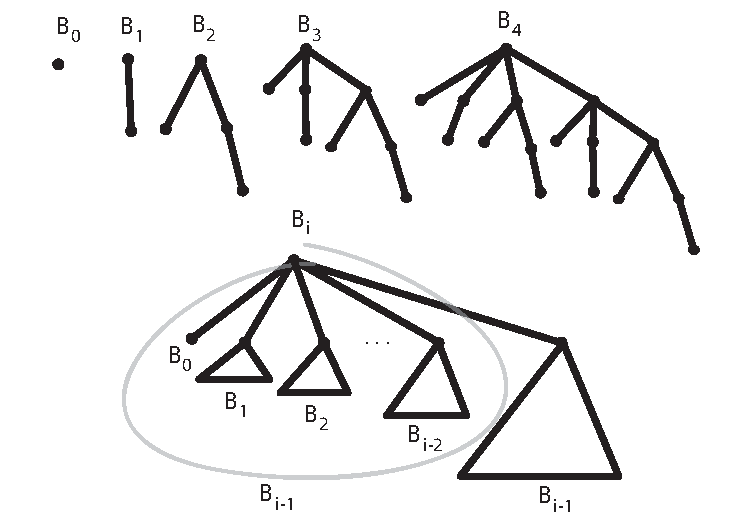
\includegraphics{pics/binheaps}
\caption{Binomi�ln� stromy}
\label{fig.heaps.binomial}
\end{figure}

\begin{tvrzeni}
Binomi�ln� halda je tvo�ena binomi�ln�mi stromy $B_i$, kter� maj� n�sleduj�c�
vlastnosti: 
\begin{itemize}
\item $B_i$ m� $2^i$ vrchol�
\item hloubka $B_i$ je i
\item ko�en $B_i$ m� i syn�
\item $\forall j < i$ existuje syn ko�ene $B_i$ takov�, �e 
  jeho podstrom je izomorfn� s $B_j$.
\end{itemize}
\end{tvrzeni}

\begin{proof}
indukc� p�es $i$ (element�rn�)
\end{proof}


\subsection{MERGE}

Algoritmus MERGE (viz algoritmus \ref{alg:heaps.binom.merge}) pracuje jako
"bin�rn� s��t�n�" - 2 stromy $B_i$ (= 2 jedni�ky v ��du $i$) slije do
$B{i-1}$ (= p�enos do $i+1$)

Pracuje v $O(\log_2 n)$ - nejvy��� mo�n� ��d je $\lfloor \log_2 n \rfloor$.
Toto je slo�itost v nejhor��m p��pad�.

Ukazatel MIN nov� haldy je nastaven na men�� z MIN($h_1$), MIN($h_2$) - to
zabere $O(1)$.


\begin{algorithm}[!htb]
\caption{MERGE pro binomi�ln� haldy}
\label{alg:heaps.binom.merge}
\begin{algorithmic}
\STATE MERGE($T_1$, $T_2$)
\STATE ($T_1, T_2$ binom. haldy velikosti $n_1,n_2$)
\STATE $P = 0, i = 0, T = 0$
\WHILE {$i \leq log(n_1 + n_2)$}
  \STATE $S_1$ je strom v $T_1$ izomorfn� s $H_i$ (pokud neexistuje, tak $S_1=0$)
  \STATE $S_1$ je strom v $T_1$ izomorfn� s $H_i$ (pokud neexistuje, tak $S_1=0$)
  % XXX \CASE
     \IF {$S_1, S_2$, P = 0}
       \STATE neprovedeme nic
     \ENDIF
     \IF {jeden strom z $S_1, S_2$, $P$ je nepr�zdn�} 
        \STATE vlo��m tento strom do $T$, $P=0$
     \ENDIF
     \IF {dva stromy z $S_1, S_2$, $P$ jsou nepr�zdn�}
       \STATE spoj�m tyto stromy a v�sledek vzlo��m do $P$
     \ENDIF
     \IF {v�echny stromy z $S_1, S_2$, $P$ jsou nepr�zdn�}
       \STATE vlo��m do $T$, spojen� $S_1, S_2$ vlo��m do $P$
     \ENDIF
  % \ENDCASE
  \STATE $i = i + 1$
\ENDWHILE
\end{algorithmic}
\end{algorithm}

\begin{pozn}
V algoritmu MERGE (viz algoritmus~\ref{alg:heaps.binom.merge}) 
odpov�d� $P$ p�enosu v bin�rn�m s��t�n�, $T$ je v�sledn� halda.
\end{pozn}

\subsection{MIN}

MIN($h$) - prohled�me prvky reprezentovan� ko�eny strom� a najdeme
nejmen��. V praxi je pro ka�dou haldu dr�en ukazatel, ukazuj�c� na ko�en
reprezentuj�c� nejmen�� prvek haldy. Tento ukazatel je obnovov�n p�i
operaci DELETE\_MIN.


\subsection{INSERT}

Operace INSERT($h$,$i$) se provede p��kazem MERGE($h$, MAKEHEAP($i$)).
Tato operace je analogick� s inkrementac� bin�rn�ho ��ta�e.

Dijkstr�v algoritmus prov�d� na za��tku $n$ operac� INSERT, n�m tedy nejde
o jednotliv� operace, ale o posloupnost INSERT�.

\begin{pozn}
INSERT je stejn� jako v leftist hald�ch.
\end{pozn}

\begin{theorem}
Amortizovan� slo�itost operace INSERT je $O(1)$.
\end{theorem}

\begin{proof}
Vyu�ijeme ��etn� metody: \\
Algoritmus INSERT udr�uje n�sleduj�c� invariant: \\
Ka�d� binom. strom v hald� m� na sv�m ��tu 1 jednotku. (Ten, kter�
p�est�v� b�t ko�enem, zaplat�, ten kdo vyhr�l, si 1 jednotku ponechal.)
P�i vytv��en� stromu ji zaplat� operace, kter� strom vytvo�ila: 
\begin{itemize}
  \item MAKEHEAP vytvo�� 1 strom $\Rightarrow$ zaplat� 1
  \item DELETE\_MIN vytvo�� $\leq log n$ strom� $\Rightarrow$ zaplat�
  	$\leq log n$
\end{itemize}
Pokud INSERT spust� kask�du sl�v�n�, pak je ka�d� slit� zaplaceno z ��tu
stromu, kter� dan�m slit�m zanikne. (jeho ko�en se stane synem)
\end{proof}


\subsection{DELETEMIN}

Operace DELETEMIN (viz algoritmus \ref{alg:heaps.binom.deletemin}) 
je provedena tak, �e ze stromu $B_k$, na kter� ukazuje
ukazatel MIN, utrhneme ko�en. T�m vzniknou nov� stromy $B_0, B_1, ...,
B_{k-1}$, ze kter�ch vytvo��me novou haldu, nastav�me pro ni ukazatel MIN
a zavol�me MERGE.

DELETEMIN pracuje v $O(log_2 n)$, proto�e $k \leq log_2 n$. Toto je
slo�itost v nejhor��m p��pad�.

\begin{algorithm}[!htb]
\caption{DELETEMIN pro binom. haldu}
\label{alg:heaps.binom.deletemin}
\begin{algorithmic}
\STATE DELETEMIN
\STATE prohled�n�m prvk� reprezentovan�ch ko�eny strom� naleznu strom $S$,
jeho� ko�en reprezentuje nejmen�� prvek
\STATE $T_1 = T \ {S}, T_2$ je tvo�en podstormy v�echn syn� ko�ene S
\STATE (tj. utrhnu ko�en a zbytek d�m do haldy) - 
	je to halda d�ky vlastnosti 4
\STATE $T \rightarrow$ MERGE($T_1, T_2$)
\end{algorithmic}
\end{algorithm}

\begin{pozn}
Operace DELETE se ned� rozumn� prov�st, museli bychom p�ebudovat cel�
strom.
\end{pozn}

\begin{theorem}
Operace MERGE, INSERT, MIN, DELETEMIN a DECREASEKEY vy�aduj� �as $O(log n)$.
Operace INCREASEKEY vy�aduje �as $O(log^2 n)$.
\end{theorem}

%\begin{pozn}
%S��t�n� v bin�rn�ch ��slech m� slo�itost $O(1)$.
%
%\begin{tabular}{|l|}
%\hline
%1 0 0 ... 0 \\
%\hline
%1 1 1 ... 1 \\
%\hline
%\end{tabular}
%\hspace{5mm}
%
%XXX amort. slo�. \\
%Neplat� n�co podobn�ho pro binom. stromy ? Ano, pro operaci INSERT.
%\end{pozn}

\begin{pozn}
MERGE zab�r� dost �asu - mus�me ho d�lat ?
\end{pozn}


\subsection{L�n� implementace binom. hald}

L�n� implementace vych�z� z toho, �e chceme operaci MERGE prov�d�t v �ase
$O(1)$.

Zm�n�me definici - vynech�me podm�nku 2 z definice \ref{def.binomheap}, 
tj. te� v na�� binom. hald� mohou b�t izomorfn� stromy. (i kdy� jen
do�asn�) Dal�� zm�na
spo��v� ve zm�n� reprezentace binomi�ln� haldy - haldu reprezentujeme
dvojit�m kruhov�m spojov�m seznamem p�es ko�eny strom�. (kruhov� spojov�
seznam umo��uje p�id�v�n� a odeb�rn� prvk� v �ase $O(1)$.)

Operaci MERGE($T_1, T_2$) pak m��eme prov�st konkatenac� seznam� $T_1$ a $T_2$.
Jenom to by nefungovalo, mus�me je�t� zm�nit operace MIN, DELETEMIN.

\begin{algorithm}[!htb]
\caption{DELETEMIN pro l�n� binom. haldy}
\label{alg:heaps.binom-line.min}
\begin{algorithmic}
\STATE MIN
\STATE p�i prohled�v�n� prvk� reprezentovan�ch ko�eny strom� se�ad�me
stromy do mno�in $Q_i$, $i=0,...,n$ , kde $Q_i$ je mno�ina v�ech strom� v
$T$ izomorfn�ch s $B_i$.
\STATE $i = 0, T = 0$
\WHILE {$\exists Q_i \neq 0$}
  \WHILE {$|Q_i| > 1$}
    \STATE vezmeme dva stromy z $Q_i$, spoj�me je, v�sledek d�me do $Q_{i+1}$
  \ENDWHILE
  \IF {$Q_i \neq 0$}
    \STATE strom z $Q_i$ d�m do $T$
  \ENDIF
  \STATE $i = i + 1$
\ENDWHILE
\end{algorithmic}
\end{algorithm}

DELETEMIN um�st� stromy po odtr�en� nejmen��ho prvku do odpov�daj�c�ch 
mno�in $Q_i$. (v mno�in� $Q_i$ jsou stromy izomorfn� s $B_i$)
Pot� provede \emph{konsolidaci} - uprav� haldu do podoby, kdy je ka�d� ��d
zastoupen nejv��e jedn�m stromem. 

Konsolidace b�� v $O(log n)$ plus vy�erp� ��ty strom�, kter� zaniknou p�i
sl�v�n�.

\begin{samepage}
Konsolidace prob�h� takto:
\begin{enumerate}
  \item vytvo��m pole d�lky $log n$, kter� je pr�zdn� 
  	$\Rightarrow$ $O(log n)$
  \item proch�z�m spojov� seznam vrchol� strom� v hald� 
  	a jeden strom za druh�m vyjmu a 
  	d�v�m do pole vytvo�en�ho v kroku 1, p�i�em� se v�dy provede 
	p��slu�n� slit�.
	\begin{itemize}
	  \item pokud strom zanikne, tak pr�ci zaplat�me z jeho ��tu
	  \item pokud strom nezanikne, tak pr�ci plat�me z ��tu
	  konsolidace $\rightarrow$ $O(log n)$
	\end{itemize}
  \item z pole vytvo��me spojov� seznam $\rightarrow$ $O(log n)$
\end{enumerate}
\end{samepage}

\begin{samepage}
DELETEMIN tedy pot�ebuje
\begin{itemize}
  \item $O(log n)$ do ��t� nov� vytvo�en�ch strom�
  \item $O(log n)$ na jejich zaveden� do spojov�ho seznamu
  \item $O(log n)$ na konsolidaci
\end{itemize}
\end{samepage}

P�i konsolidaci v�dy z�rove� vyhled�me nov� minimum.

\begin{theorem}
Operace MERGE a INSERT p�i l�n� implementaci vy�aduj� �as $O(1)$, operace
DELETEMIN a MIN vy�aduj� �as $O(\text{po�et strom� v hald�})$.
\end{theorem}

%\begin{pozn}
%$bal(\text{konfigurace}) = \text{po�et v�ech strom� ve v�ech hald�ch v
%konfiguraci}$
%\end{pozn}
%
%\subsubsection{Amort. slo�.}
%$\text{amort. slo�.} = \text{�as pro operaci} + 
%bal(\text{v�sledn� konfigurace}) - bal(\text{p�vodn� konfigurace})$

\vspace{5mm}

\begin{center}
\begin{tabular}{|l|l|}
\hline
Operace & Amort. slo�itost \\
\hline
MERGE & $O(1)$ \\
INSERT & $O(1)$ \\
MIN & $O(log n)$ \\
DELETEMIN & $O(log n)$ \\
\hline
\end{tabular}
\tabcaption{Amortizovan� slo�itost pro l�n� binomi�ln� haldy}
\label{tab:binheaps.lazy.complexity}
\end{center}

% \subsection{Zobecn�n� binomi�ln� haldy}

% XXX
% \mnote{p�edn�elo se to tento rok (2004) v�bec ?}

% --------------------------------------------------------------------------
\section{Fibonacciho haldy}

Fibonacciho haldy vych�zej� z binomi�ln�ch hald, form�ln� se li�� v podstat�
pouze t�m, �e v hald� povol�me i jin� stromy ne� binomi�ln�. Toto n�m
umo�n� implementaci operace DECREASE\_KEY, kter� nebyla v binomi�ln�ch
hald�ch p�i zachov�n� slo�itosti ostatn�ch operac� mo�n�.

��d uzlu a stromu je definov�n jako u binomi�ln�ch hald. Sl�v�n� se
prov�d� pouze mezi stromy stejn�ho ��du.

\subsection{MERGE, INSERT, EXTRACT\_MIN}

Implementace operac� MERGE($h_1$,$h_2$), INSERT($h$,$i$), EXTRACT\_MIN($h$) 
je stejn� jako u binomi�ln�ch hald v "l�n�" verzi.

\subsection{DECREASE\_KEY}

DECREASE\_KEY prov�d� sn��en� hodnoty kl��e pro dan� prvek. To se d�je za
cenu p��tomnosti jin�ch ne� binomi�ln�ch strom� v hald�.

\begin{algorithm}[!htb]
\caption{DECREASE\_KEY pro Fibonacciho haldy}
\label{alg:heap.fib.decrease_key}
DECREASE\_KEY($h$,$i$,$\delta$)
\begin{enumerate}
  \item sn���m kl�� prvku $i$ o $\delta$
  \item podstrom i s ko�enem $i$ od��zneme a jako samostatn� strom ho
        zavedeme haldy (tj. za�ad�m do spojov�ho seznamu ko�en� strom� v
	hald�) $\Rightarrow$ $O(1)$
  \item Abychom udr�eli stromy dostate�n� "ko�at�"\footnote{nechceme 
  	stromy typu "smet�k" - tj. takov�ch, kter� sest�vaj� pouze 
	z ko�ene a jeho syn�, kter� jsou z�rove� listy}
  	tak od ka�d�ho vrcholu $x$ mohou b�t od��znuti nejv��e 2
  	synov� $\Rightarrow$ po od��znut� 2. syna je od��znut i s�m vrchol $x$.
\end{enumerate}
\end{algorithm}

\begin{figure} 
\centering\includegraphics{pics/fibheaps}
\caption{Po�ty vrchol� strom� $F_0, F_1, ...$ tvo�� Fibonacciho
posloupnost.}
\label{fig:heaps.fib.pocty.vrcholu}
\end{figure}

\begin{pozn}
P�esto�e jedna operace DECREASE\_KEY m��e vyvolat kask�du �ez�, je jej�
amortizovan� slo�itost $O(1)$.
\end{pozn}

\begin{pozn}
Pomoc� \emph{��etn� metody}\footnote{Pro definici ��etn� metody viz
p�edn�ky ze "\emph{Slo�itosti a NP �plnosti}".}
dok�eme, �e to plat�: \\
P�i od�ez�v�n� syna vrcholu $x$ zaplat� operace DECREASE\_KEY
\begin{samepage}
\begin{itemize}
  \item 2 jednotky na ��et $x$
  \item 1 jednotku na ��et vznikl�ho stromu
  \item 1 jednotku za pr�ci (od��znut� a za�azen�)
\end{itemize}
\end{samepage}

P�i od��znut� druh�ho syna jsou na ��tu vrcholu $x$ 4 jednotky
$\Rightarrow$ mohu zopakovat body 1) - 3).
\end{pozn}

\begin{theorem}
\label{heaps.fib.theorem}
Nejvy��� ��d stromu ve Fibonacciho hald� je $\lfloor log_\varphi n \rfloor =
\Theta(log_2 n)$ pro n�jak� $\varphi > 1$.
\end{theorem}

\begin{lemma}
\label{heaps.fib.lemma}
Nech� $x$ je vrchol a $y_1, ..., y_m$ jeho synov� v po�ad�, v jak�m byli k
$x$ sliti. Potom $\forall \in {1,...,m}$ je ��d $y_i$ aspo� $i-2$.
\end{lemma}

\begin{proof}
V okam�iku, kdy byl $y_i$ slit pod $x$, m�l $x$ ��d $\geq i-1$.
($y_1,...,y_{i-1}$ ji� v t� chv�li byli synov� $x$)
V tomto okam�iku byl tak� ��d $y_{i-1} \geq i-1$. (sl�v�me pouze stromy
stejn�ho ��du) Od t� doby mohl $y_i$ ztratit nejv��e jednoho syna, jinak
by byl s�m od��znut a p�estal by b�t synem $x$. $\Rightarrow$ $y_i$ m� ��d
$\geq i-2$. 
\end{proof}

\begin{proof}
Dokazujeme v�tu \ref{heaps.fib.theorem}, kter� jin�mi slovy ��k�: 
Strom ��du $i$ ve
Fibonacciho hald� m� velikost alespo� $\varphi^i$ pro n�jak� $\varphi >
1$.

Nech� $F_j$ je nejmen�� mo�n� (tj. m� o�ezan� podstromy na max. mo�nou
�rove� - byl z nich od��znut 1 syn) strom ��du $j$ spl�uj�c� tvrzen� lemma
\ref{heaps.fib.lemma} a nech� $|F_j| = f_j$. Pak

\begin{enumerate}
  \item $F_i$ vznikne "slit�m" $F_{i-1}$ a $F_{i-2}$ $\Rightarrow$ 
  	$f_i = f_{i-1} + f_{i-2}$
  \item $f_i \geq \varphi^i$, kde 
  	$\varphi = \frac{1+\sqrt 5}{2} \approx 1.618$ ... zlat� �ez
\end{enumerate}

\begin{itemize}
  \item[ad 1)] 
  viz obr.~\ref{fig:heaps.fib.proof}

  \begin{figure} 
  \centering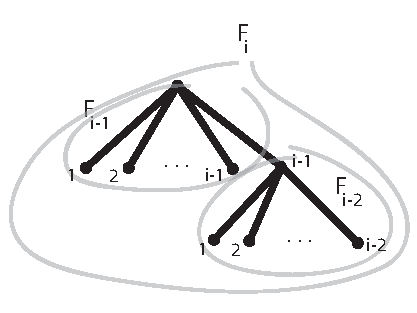
\includegraphics{pics/fibheap}
  \caption{K d�kazu v�ty \ref{heaps.fib.theorem}}
  \label{fig:heaps.fib.proof}
  \end{figure}

  Slit� je nep�esn� term�n - sl�v�me pouze stromy stejn�ho ��du.
  $F_{i-2}$ je v�sledek DECREASE\_KEY. (t�m se strom "oholil") U��znu
  posledn�ho syna, pod kter�m je nejv�t�� podstrom (abych dostal nejmen��
  mo�n� podstrom)

  \item[ad 2)]
  $\varphi$ je klad� ko�en rovnice $x^2 - x - 1 = 0$ \\
  neboli plat� $\varphi^2 = \varphi + 1$, $\varphi = \frac{1+\sqrt 5}{2}
  \approx 1.618$ \\
  dok�eme indukc�: 
    \begin{itemize}
      \item i = 0 : $f_0 = 1 \geq \varphi^0 = 1$
      \item i = 1 : $f_1 = 2 \geq \varphi^1 = 1.618$
      \item induk�n� krok: IP: $f_i \geq \varphi^i$, $f_{i+1} \geq
      \varphi^{i+1}$ \\
        $f_{i+2} = f_{i+1} + f_i \geq \varphi^{i+1} + \varphi^i =
	\varphi^i(\varphi + 1) = \varphi^{i+2}$
    \end{itemize}
\end{itemize}
\end{proof}



% ==========================================================================
% Sou��st skript na Datov� struktury. Viz main.tex
\markright{$ $Id$ $}
% doplnil Vladim�r Kotal

\chapter{Dynamizace}

V uspo��dan�m poli um�me rychle vyhled�vat, ale p�idat prvky znamen�
cel� ho p�ebudovat. Ve str�staj�c�m ha�ov�n� zase ne�ly prvky mazat,
ve velmi komrimovan�ch trie ani p�id�vat, ani mazat. V t�to kapitole
uk�eme obecnou metodu, jak tyto probl�my �e�it, podobnou p��stupu u
binomi�ln�ch hald.

% --------------------------------------------------------------------------
\section{Zobecn�n� vyhled�vac� probl�m}

\begin{defn}
\emph{Vyhled�vac� probl�m} je funkce $f: U_1 \times 2^{U_2} \to U_3$, kde
$U_1$, $U_2$ a $U_3$ jsou univerza.
\end{defn}
\begin{defn}
\emph{�e�en� vyhled�vac�ho probl�mu} pro $x \in U_1, A \subseteq U_2$
je nalezen� hodnoty $f(x, A)$.
\end{defn}

\begin{pozn}
Chceme naj�t strukturu, kter� reprezentuje A a algoritmus, kter� pro vstup
$x \in U_1$ spo��t� $f(x, A)$. Takov� struktu�e se ��k� statick� struktura
pro vyhled�vac� probl�m.
\end{pozn}

P�.:
\begin{description}
\item[Klasick� vyhled�vac� probl�m:]

	$U_1 = U_2 = U$, univerzum prvk�;
	$U_3 = \{0, 1\}, A \subseteq U_2$

	$f(x, A) =
	\begin{cases}
	0& \text{kdy� } x \notin A\\
	1& \text{kdy� } x \in A
	\end{cases}$
	(rozlo�iteln�)
\item[Euklidovsk� vzd�lenost bod� v rovin�:]

	$U_1 = U_2 = $ euklidovsk� rovina; 
	$U_3 = \mathbb{R}^+$; 
	$f(x, A) = dist(x,A$ vzd�lenost bodu $x \in U_1$ od mno�iny $A$.
	(rozlo�iteln�, $\oplus$ ... operace min)
\item{Nalezen� p�edch�dce}
	$U_1 = U_2 = U_3$ 
	pro $x \in U_1$ a $A \subseteq U_!$ a je $f(x,U_!)$ je nejv�t�� 
		prvek $A \leq x$
	(rozlo�iteln�, je pot�eba disjunkce)
\item[P��slu�nost ke konvexn�mu obalu]

	$U_1 = U_2 = $ rovina; 
	$U_3 = \{0, 1\}$;

	\(f(x, A) =
	\begin{cases}
	0& \text{kdy� $x$ nepat�� do konvexn�ho obalu $A$}\\
	1& \text{kdy� $x$ pat�� do konvexn�ho obalu $A$}
	\end{cases}\)
	(nen� rozlo�iteln� probl�m)
% XXX obr.
\end{description}


\subsection{Operace INSERT a DELETE}
Pro mno�inu $A \subseteq U_2$ a pro statickou strukturu {\cal S}
�e��c� vyhled�vac� probl�mf pro $x \in U_2$.
INSERT(x,A) - vybudov�n� struktury �e��c� vyhled�vac� probl�m pro mono�inu
$A \cup \{x\}$.
DELETE(x,A) - vytvo�en� struktury �e��c� vyhl. probl�m pro mno�inu 
$A - \{x\}$.

Pozn:
ze statick� struktury chce vytovo�it dynamickou (dynamizace).INSERT je
obvykle jednodu��� ne� DELETE, na tu budeme pot�eboivat dodate�n�
p�edpoklady.

N�roky na dynamizaci
- chceme aby se f(x,A) v nov� struktu�e spo��talo p�ibli�n� stejn� rychle
  jako v p�vodn� struktu�e
- kdy� vytvo�en� p�vodn� struktury pro n prvnkovou mno�inu trvalo
  t, pak operace INSERT by p�ibli�n� m�la vy�adovat �as t $t/n$.

\begin{defn}
Vyhled�vac� probl�m je \emph{rozlo�iteln�}, kdy�
existuje operace $\oplus$ spo�itateln� v konstantn�m �ase a plat�:
kdy� $x \in U_1$ a $A$ a $B$ jsou disjunktn� podmno�iny $U_2$, pak
\[
	f(x, A \cup B) = f(x, A) \oplus f(x, B).
\]
\end{defn}

\begin{pozn}
Z v��e uveden�ch p��klad� nen� rozlo�iteln�m probl�mem p��slu�nost ke
konvexn�mu obalu, ostatn� vyhled�vac� probl�my jsou rozlo�iteln�.
\end{pozn}

\newcommand{\staticka }{\ensuremath{\mathcal{S}}}
\newcommand{\dynamicka}{\ensuremath{\mathcal{D}}}


\begin{defn}
Nech� $f$ je rozlo�iteln� vyhled�vac� probl�m a $\staticka$ je
``statick�'' datov� struktura, kter� ho �e��. Neboli $\staticka$ je
tvo�ena pro pevnou mno�inu $A \subseteq U_2$ a obsahuje operaci, kter�
pro vstup $x$ po��t� $f(x, A)$.

Pop��eme d�le�it� parametry $\staticka$: nech� $n = |A|$, ozna�me
\begin{align*}
Q_\staticka(n) & = \text{�as pot�ebn� pro v�po�et $f(x,A)$}\\
S_\staticka(n) & = \text{pam� pot�ebn� pro vybudov�n� \staticka}\\
P_\staticka(n) & = \text{�as pot�ebn� pro vybudov�n� \staticka}
\end{align*}
\end{defn}

Budeme p�edpokl�dat, �e $Q_\staticka(n)$, $S_\staticka(n)/n$ a
$P_\staticka(n)/n$ jsou neklesaj�c� funkce.

M�me mno�inu A a vytvo��me pro ni novou strukturu D.
Nech� $A_i \subseteq A$ takov�, �e bu� $|A_i| = 2^i$ nebo $A_i = \emptyset$ \\
$A_i \cap A_j = \emptyset pro i \neq j$.
$\bigcup A_i = A$

Plat� $A_i \neq \emptyset$ pr�v� kdy� (i+1)-n� bit v dvojkov�m rozvoji ��sla
|A| je 1.

Chceme navrhnout strukturu, kter� by um�la
\begin{enumerate}
\item Pro $x \in U_1$ a pevn� $A \subseteq U_2$ rychle spo��tat $f(x, A)$.
\item Pro $A$ a $y \in U_2$ rychle vytvo�it strukturu pro $A \cup \{y\}$.
\end{enumerate}

M�jme $A_0, A_1, \cdots$ takov�, �e
\begin{enumerate}
\item $A_i \cap A_j = \emptyset$ pro $i \neq j$
\item bu� $A_i = \emptyset$ nebo $|A_i| = 2^i$ 
\item $\bigcup_i A_i = A$ 
\end{enumerate}

Nov� struktura \dynamicka\ reprezentuj�c� $A$ je potom
\begin{itemize}
% \item Seznam statick�ch struktur pro $A_i \neq \emptyset$, $\staticka_i$
\item n�jak� dynamick� struktura reprezentuj�c� A
(nap�. (a,b)-strom, �erveno-�ern� strom, AVL-strom)
% \item Vyhled�vac� strom reprezentuj�c� $A$
\item Pro ka�d� $A_i \neq \emptyset$ m�me S strukturu reprezentuj�c� $A_i$.
\item Pro ka�d� $A_i \neq \emptyset$ seznam prvk� v $A_i$; prvky
t�chto seznam� jsou projpojeny s odpov�daj�c�mi prvky ve strom�.
\end{itemize}

Jak v nov� struktu�e spo��t�me f(x,A) ?
pro ka�dou $A_i \neq \emptyset$ spo��t�me $f(x,A_i)$ a pomoc� operace
$\oplus$ pak spo��t�me f(x,A).

\begin{pozn}
 plat�, kdy� $A_i \neq \emptyset$, pak 
$i \leq \lceil log_2|A| \rceil$
�as, kter� je pot�eba v nov� struktu�e na v�po�et f(x,A)
\end{pozn}

\begin{multline}
log_2|A| + \sum_{i=0}^{log|A|}Q(2^i) \leq log|A| + \sum_{i=0}^{log|A|}Q(|A|)
= log|A|(Q(|A|) + 1)
\end{multline}

$log_2(|A|)$ - vyhodnocen� $f(x,A)$ z $f(x,A_i), i=0,1,...$
\par

tedy algoritmus pot�ebuje O(log|A| Q(|A|)) �asu
kdy� $Q(n) = \Theta(n^\epsilon) pro \epsilon > 0$, pak plat�. �e nov�
struktura pro v�po�et f pot�ebuje
\begin{multline}
log|A| + \sum_{i=0}^{log n}Q(2^i) = \\
|A| + \sum_{i=0}^{log|A|}
\frac{S(2^i)}{2^i} 2^i \leq |A| + \sum_{i=0}^{log|A|} \frac{S(|A|)}{|A|} 2^i \\
= |A| - \frac{S(|A|)}{|A|} 2^i = |A| -
\frac{S(|A|)}{|A|}(\sum_{i=0}^{log|A|} 2^i) \\
= O(S(|A|))
\end{multline}


INSERT(x)
\begin{algorithmic}
\IF {$x \not\in A$} 
  \STATE nalezneme nejmen�� j, �e $A_j = \emptyset$
\ENDIF
\STATE $A_j = \{x\} \cup \bigcup{i<j} A_i, A_i = \emptyset pro i<j$
\STATE vytvo��me strukturu S spojov� seznam pro $A_j$
\STATE x p�id�me do reprezentace A.
\end{algorithmic}


Kdy se buduje znovu S struktura pro $A_j$ ? 
\begin{enumerate}
\item mus� se naplnit v�echny $A_i$ pro i<j 
to je $2^{j-1}$ �sp�n�ch INSERT� (ty, kter� p�idaly prvek)
\item provede se �sp�n� INSERT, kter� vypr�zdn� $A_i$ pro $i \leq j$
\item znovu se mus� naplnit $A_i$ tj. $2^{j-1}-1$ �sp�n�ch INSERT�
\item da�� �spe�n� INSERT vytvo�� teprve S strukturu pro $A_j$
\end{enumerate}

tj. $2 \cdot 2^j$ �sp�n�ch INSERT�

\subsection{Amortizovan� �as operace INSERT}
$$
log|A| + \sum_{i=0}^{log|A|} \frac{P(2^j)}{2^{j+1}} \leq
log|A| + \sum_{i=0}^{log|A|} \frac{P|A|}{|A|} = 
O(log|A| \cdot \frac{P|A|}{|A|})
$$

\begin{pozn}
pokud $\frac{P(n)}{n} = \Theta(n^\epsilon) pro \epsilon > 0$, pak
amortizovan� �as pro operaci INSERT bude $O(\frac{P|A|}{|A|})$.
\end{pozn}

\begin{theorem}
M�me rozlo�iteln� vyhled. probl�m f a m�me pro n�j statickou strukturu,
kter� ho �e�� v �ase $Q(n)$, vy�aduje $S(n)$ pam�ti a vytvo�� se v �ase
$P(n)$,
$kde Q(n), \frac{P(n)}{n}, \frac{S(n)}{n}$ jsou neklesaj�c� funkce. Pak
jsme navrhli novou semidynamickou dat. strukturu D, �e��c� f v �ase
$O(Q(n) log(n))$ vy�aduj�c� $O(S(n))$ pam�ti a umo��uj�c� INSERt s 
amort. slo�itost�
$O(\frac{P(n)}{n} \cdot log(n))$.
\end{theorem}

M�me mno�inu A \\
budeme m�t roklad A na disjunktn� mno�iny $A_{i,j}, i=0,1,..., j \in
{0,1,...,k_j}$, kde $k_j \in {0,1,2}$. \\
$|A_{i,j}| = 2^i$ a plat�: \\
kdy� $A_{i,0}$ existuje pro $i > 0$, pak existuj� $A_{i-1,0}, A_{i-1,1}$.
\par

Struktura: 
\begin{enumerate}
\item reprezentace A (pomoc� (a,b)-strom�, �erveno-�ern�ch strom�, ...)
\item $\forall$ existuj�c� $A_{i,j}$ je S struktura reprezentuj�c�
$A_{i,j}$ 
\item $\forall$ existuj�c� $A_{i,j}$ je spojov� seznam reprezentuj�c�
$A_{i,j}$
\item kdy� $A_{i,0}$ a $A_{i,1}$ existuj� pro n�jak� i, pak je 
"rozpracovan�" S struktura pro mno�inu $A_{i-1,k_i+1} = A{i,0} \cup
A_{i,1}$.
tj. bylo provedeno n�kolik krok� pro jej� vytvo�en�, ale nen� dokon�ena.
\end{enumerate}


% ==========================================================================
\chapter{V�cedimenzion�ln� vyhled�v�n�}



% ==========================================================================
\end{document}
